%\documentclass[pdftex,a4paper,12pt]{scrreprt}
\documentclass[pdftex,a4paper,12pt]{scrreprt}
\usepackage{ngerman}
%\documentclass[pdftex,a4paper,12pt]{scrbook}
\usepackage[latin1]{inputenc} 
%\usepackage[utf8]{inputenc} 
\usepackage[bibcomment]{tntdasa}
\usepackage{hyperref}
\usepackage{graphicx}
\usepackage{subfigure}
\usepackage{enumerate}
\usepackage{pdflscape}
\usepackage{booktabs}
\usepackage{url}

\usepackage{array}
\usepackage{mathtools}
\usepackage{makeidx}
\usepackage{times}
\usepackage{amssymb}
\usepackage{amsmath}
%\hyphenation{german}
\usepackage{inputenc}

\usepackage{epstopdf}
\usepackage{mathrsfs}
\usepackage{etoolbox}

%\usepackage{hyperref}
%\usepackage{acronym}

\apptocmd{\thebibliography}{\csname phantomsection\endcsname\addcontentsline{toc}{chapter}{\bibname}}{}{}
\usepackage{float}
\usepackage{subfigure}
\usepackage[numbers]{natbib}
%\usepackage{slashbox} % make backslash in the table
\usepackage{setspace}
\usepackage{algorithm}
\usepackage{algorithmic}
\usepackage{multirow}
\usepackage{units}
\usepackage{textcomp}
\usepackage{bigfoot}
\usepackage{pdflscape}
%\usepackage{hyperref}
%\hypersetup{
%           colorlinks = true,
%    linkcolor=black,        % color of internal links (change box color with linkbordercolor)
%    citecolor=red,        % color of links to bibliography
%    filecolor=magenta,      % color of file links
%    urlcolor=cyan           % color of external links
%}

 \newlength{\subfigwidth}
  \setkeys{Gin}{width=\subfigwidth}

  \def\setcols#1{%
    \setlength{\subfigwidth}{\linewidth}%
    \addtolength{\subfigwidth}{\tabcolsep}
    \addtolength{\subfigwidth}{-#1\tabcolsep}
    \divide\subfigwidth by#1}
%    
\newcommand{\argmin}{\operatornamewithlimits{argmin}}
\newcommand{\argmax}{\operatornamewithlimits{argmax}}   
 
\renewcommand{\algorithmicrequire}{\textbf{Input:}}
\renewcommand{\algorithmicensure}{\textbf{Output:}}
\renewcommand{\bibname}{Bibliography}

\renewcommand{\contentsname}{Contents}
\renewcommand{\listfigurename}{List of Figures}
\renewcommand{\listtablename}{List of Tables}
\renewcommand{\figurename}{Figure}
\renewcommand{\tablename}{Table}


\newcommand\DAGMreviewversion{
  \usepackage{lineno}
  \usepackage{color}
  \renewcommand\thelinenumber{\color[rgb]{0.2,0.5,0.8}\normalfont\sffamily\scriptsize\arabic{linenumber}\color[rgb]{0,0,0}}
  \renewcommand\makeLineNumber {\hss\thelinenumber\ \hspace{6mm} \rlap{\hskip\textwidth\ \hspace{6.5mm}\thelinenumber}} 
  \linenumbers
}
%
\pagestyle{tntdasa}

\newcolumntype{L}[1]{>{\raggedright\let\newline\\\arraybackslash\hspace{0pt}}m{#1}}
\newcolumntype{C}[1]{>{\centering\let\newline\\\arraybackslash\hspace{0pt}}m{#1}}
\newcolumntype{R}[1]{>{\raggedleft\let\newline\\\arraybackslash\hspace{0pt}}m{#1}}

%******************************************************************************
\begin{document}
%\frontmatter%
\tntdasatitle{Masterarbeit}                % Diplom/Studienarbeit
             {Gaussian Processes for Video Surveillance Activity Recognition}  % Titel der Arbeit
             {Wentong Liao}    % Name des Studenten
             {Matrikelnummer: 2906540}    % Name des Studenten
             {Dr.-Ing. Michael Yang}    % Betreuer
             {Prof. Dr.-Ing. Bodo Rosenhahn}% Erstprüfer
             {Prof. Dr.-Ing. J"orn Ostermann}% Zweitprüfer
             {Hannover, Mai 2015}         % Ort,Datum (Titelseite) 
             {Hannover, den 18.05.2015}    % Ort,Datum (Erklärung)


%******************************************************************************
\setlength{\oddsidemargin}{1cm}
\setlength{\evensidemargin}{-1cm}
%******************************************************************************


\chapter*{Abstract}
\label{chap:Abstract}
\addcontentsline{toc}{chapter}{Abstract}
\setcounter{page}{1}
\pagenumbering{roman}
%******************************************************************************
In this thesis we mainly discuss  the solutions for visual relation detection.To find the solutions, we need to not only develop models that detect the objects in an image, but also predict the interactions between the detected objects. Therefore, a comprehensive scene understanding of an image would be considered in aspect of connecting computer vision and natural language  helpful. Even though the work in field of deep learning has been quite accomplished, but it remaining to be a complex and challenging task to extract related scene information. 

 Inspired by the contemporary achievement of transformer in computer vision, we propose Retina Net, which was based transformer structure designed . In order to meet different requirements in visual relation detection, we designed specific object query with physical meanings. The specific object query is capable of extracting better object features in an image with the help of our attention loss.  By taking into account global context, we also model relation to object interactions through our designed relation decoder. We attempt a lot to find the mechanism of attention in the models and to understand which details should be paid more attention to when it comes to relation predicts.
 
 To our best effort, by using transformer structure our study for the first time try to complete all the models of relation detection . It is a new approach to solve the problems. The results of our experiments indicate that our models solve the tasks in visual relation detection properly.

%------------------------------------------------------------------------
%-------------------------------------------------------------------------

%******************************************************************************
\chapter*{Kurzfassung}

%------------------------------------------------------------------------
%-------------------------------------------------------------------------

%******************************************************************************
\label{chap:Kurzfassung}
\addcontentsline{toc}{chapter}{Kurzfassung}

In dieser Arbeit 
%*******************************************************************************************

%*****************************************************************************************
\tableofcontents

\addcontentsline{toc}{chapter}{List of Tables}
\listoftables

\addcontentsline{toc}{chapter}{List of Figures}
\listoffigures
%\addtocontents{lof}{\bfseries\Large Figures\vskip10pt}
%\caption[Short version for listoffigures]
%****************************************************************************************

\hypersetup{
    colorlinks = true,
    linkcolor=blue,          % color of internal links (change box color with linkbordercolor)
    citecolor=red,        % color of links to bibliography
    filecolor=magenta,      % color of file links
    urlcolor=cyan           % color of external links
}
%========================================================================================


\chapter{Introduction}
\label{chap:introduction}
\setcounter{page}{1}
\pagenumbering{arabic}

In recent years, computer vision has made great progress. People have achieved good results in some simple tasks and have been applied in many fields, such as image classification~\cite{yu2017convolutional, lu2007survey}, image segmentation ~\cite{pham2000current} and face recognition~\cite{ahonen2006face, phillips1996feret}. Now people are no longer satisfied with these basic tasks, but hope that computers can interpret pictures like humans to obtain more information, such as the attributes of objects,  the motion of objects, and the relationships between objects, etc. Thus people began to study some complex tasks such as mage Captioning ~\cite{hossain2019comprehensive},  Visual Question Answer~\cite{antol2015vqa}, and  visual relationship detection (VRD). \\

\begin{figure}[!htbp]
	\centering
	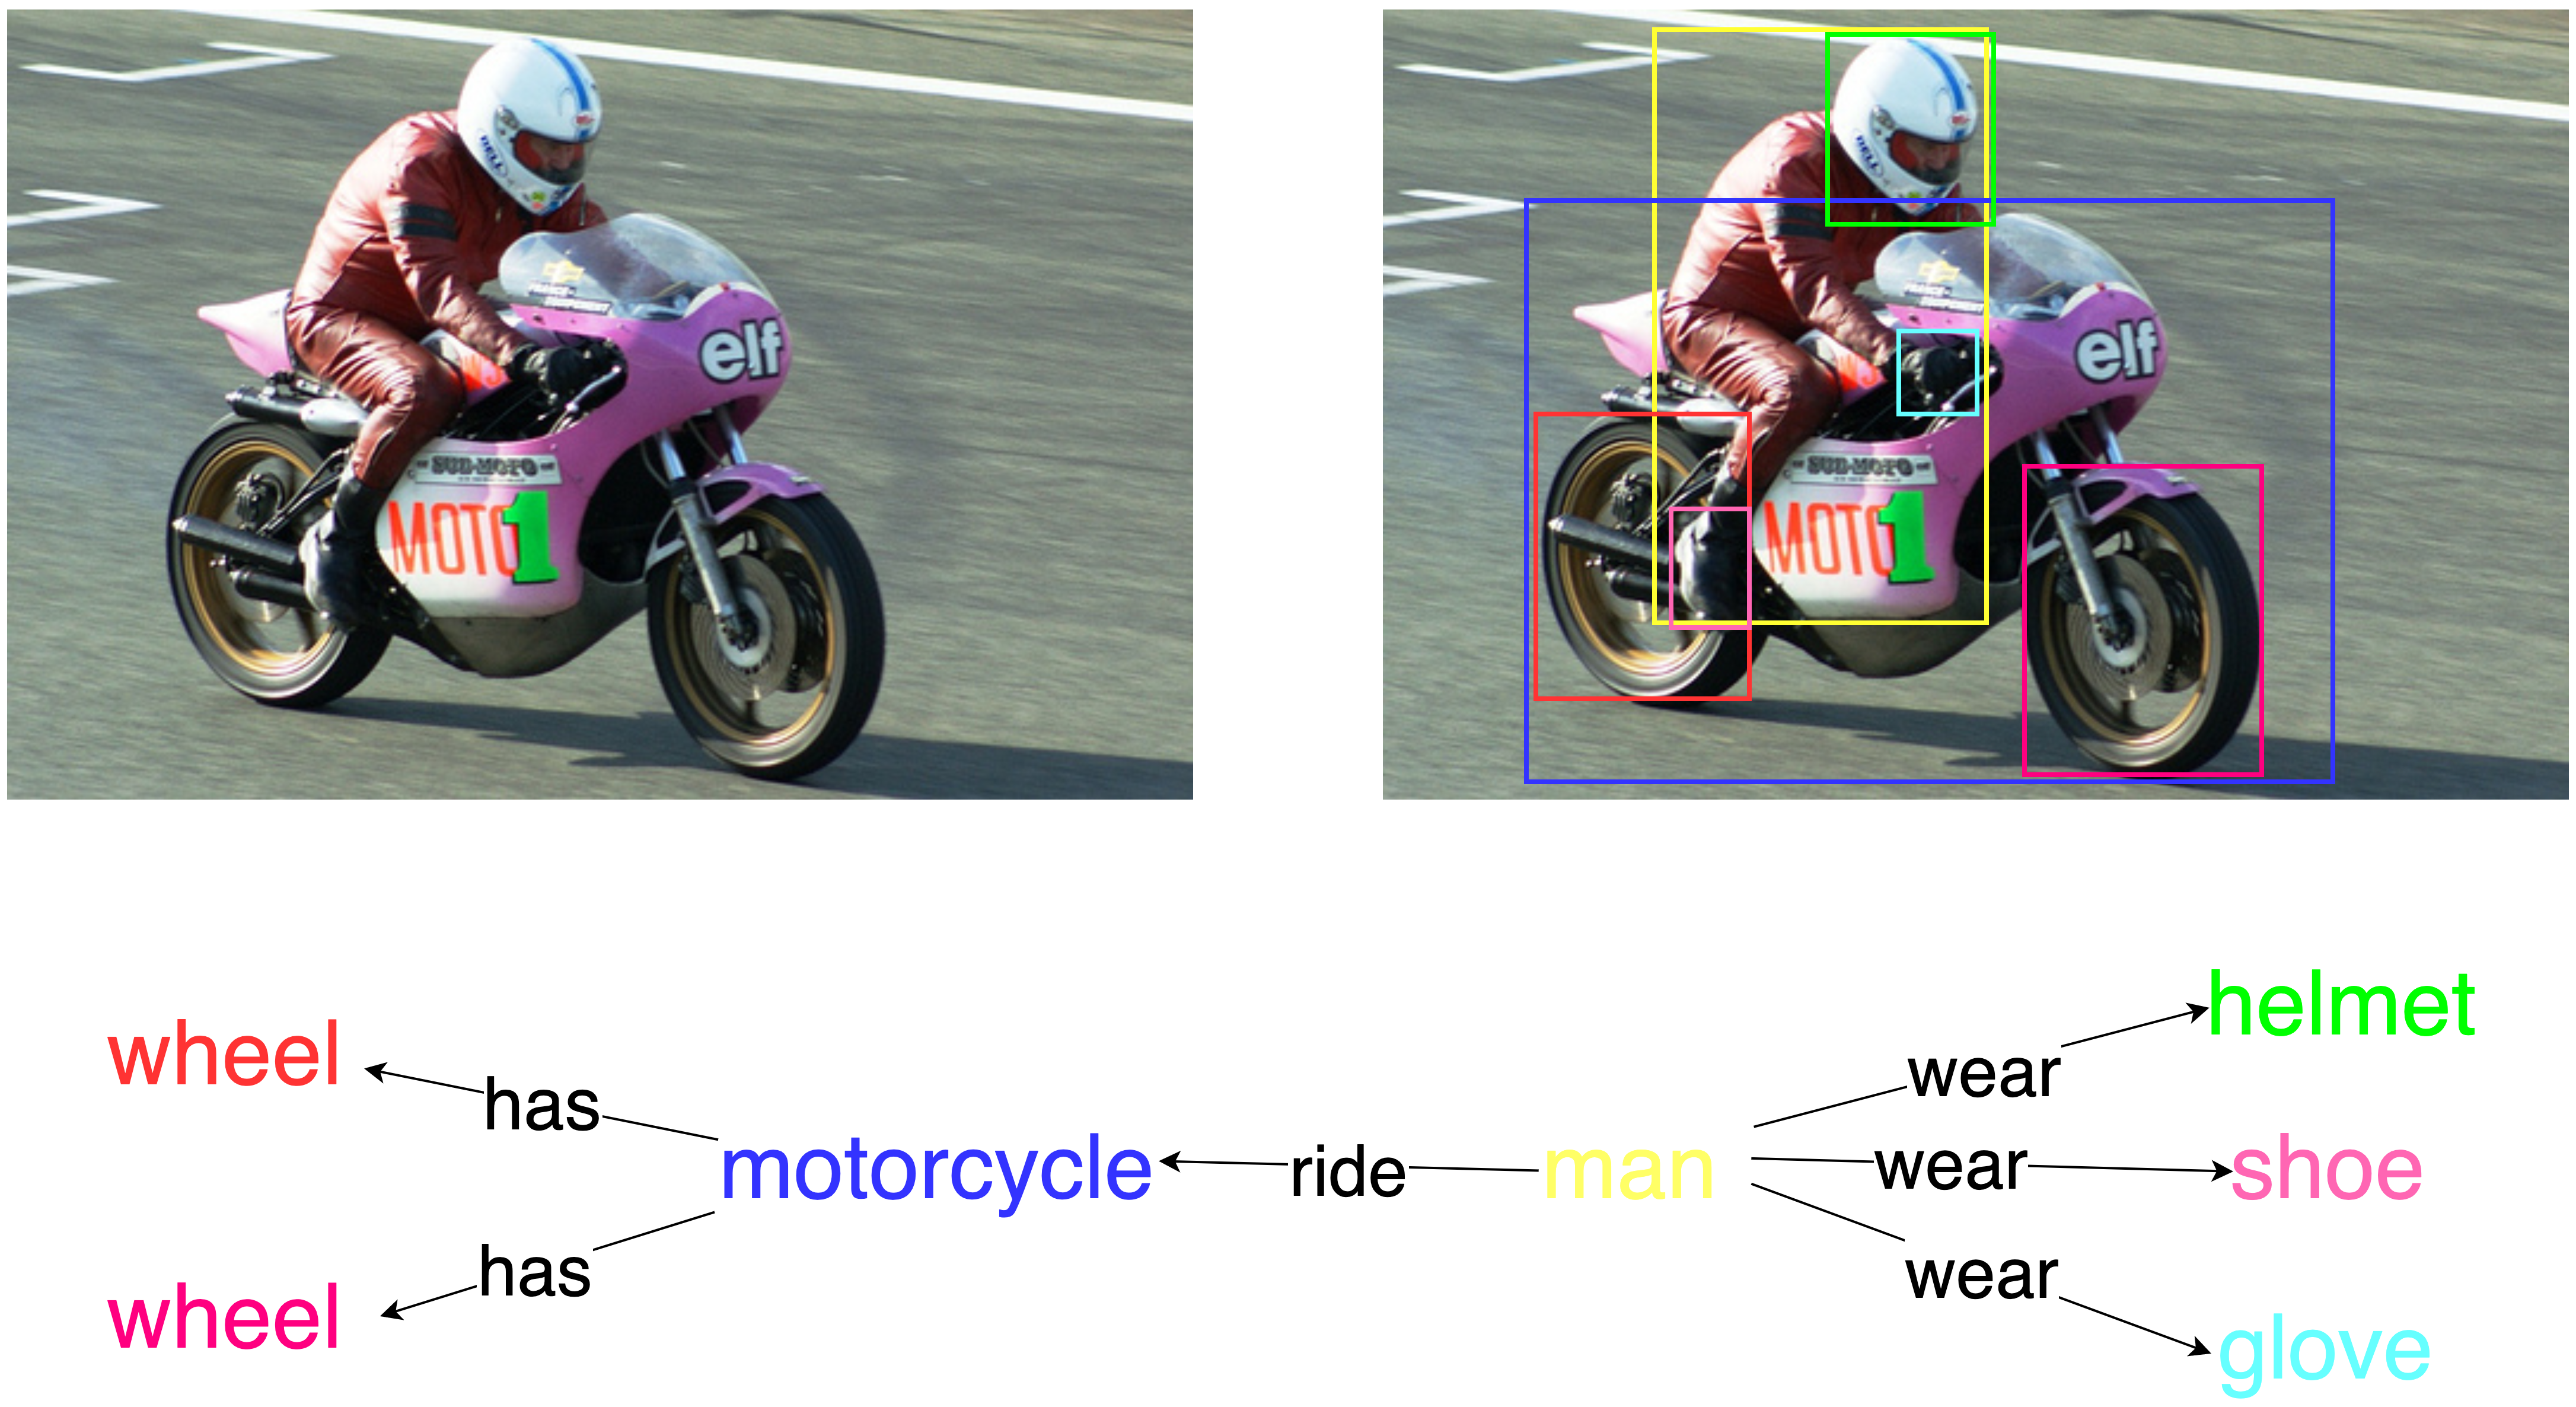
\includegraphics[width = 0.9 \textwidth]{figures/senen_graph.png}
	\caption[A example of visual relationship detection]
	{ A example of visual relationship detection: The upper left corner is the original input image, the upper right corner is the result of object detection, and the lower one is the relationship detection}
	\label{fig:sene}
\end{figure}

The visual relationship detection task not only needs to recognize the objects in the image and their positions, but also recognize the relationship between the objects, that is, the connection between the target objects, which can be expressed as a triplet-Relationship: $\left \langle subject, predicate, object\right \rangle$. For example, in figure~\ref{fig:sene}, a VRD task includes identifying instances in the image: motorcycle, man, helmet, wheels, etc., as well as identifying the relationship between them, like $\left \langle man, ride, motorcycle\right \rangle$, $\left \langle man, wear, helmet\right \rangle$, $\left \langle motor, has, wheel\right \rangle$, etc..




\section{Motivation}

Visual relationship detection connects objects in images with predicates, and also connects low-level vision and high-level language (see Figure ~\ref{fig:vrd}). This means that visual relationship detection can provide high-level tasks, such as image subtitles [7] for easier-to-understand information; it can also improve low-level tasks such as object detection using scene context. Visual relationship detection is an essential step to realize that computers can understand images as intelligently as humans.

\begin{figure}[!htbp]
	\centering
	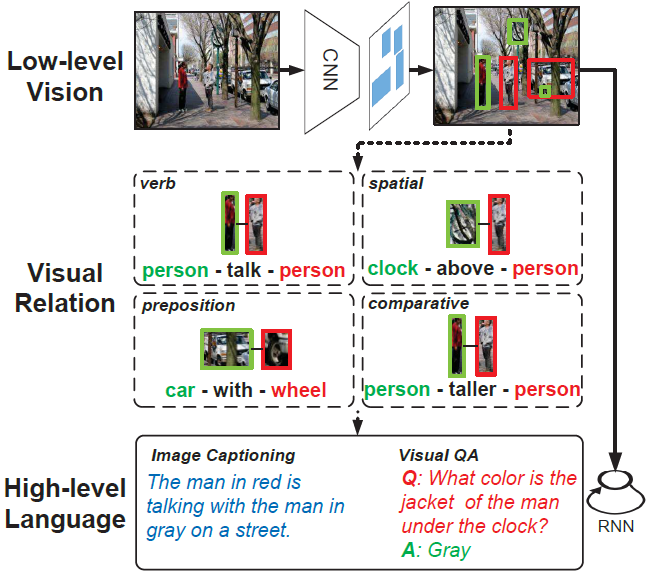
\includegraphics[width = 0.9 \textwidth]{figures/VRD.png}
	\caption[Connection between low-level vision and high-level vision]
	{ Visual relationship detection understands object interactions directly, which offer further semantic information for applications such as image captioning and QA. Figure obtained from ~\cite{zhang2017visual}}
	\label{fig:vrd}
\end{figure}

In recent years, with the proposal of the Transformer structure~\cite{vaswani2017attention}(see in section~\ref{section:transformer}), people have found that it not only achieves excellent performance in natural language processing tasks, but also has a very wide range of applications in computer vision, such as the DETR model~\cite{carion2020end} (see Figure ~\ref{fig:detr})proposed by Nicolas et al., using the Encoder-Decoder structure of the Transformer, The object detection effect of DETR is not inferior to Faster R-CNN~\cite{ren2016faster}. Thus we want to study the possibility of transformer structure in VRD problem.

\begin{figure}[!htbp]
	\centering
	\includegraphics[width = 1 \textwidth]{figures/DETR.png}
	\caption[The framework of DETR model]
	{ The framework of DETR model. Figure obtained from ~\cite{carion2020end}}
	\label{fig:detr}
\end{figure}


There are three main related tasks of visual relationship detection task: Predicate classification, which only needs to predict the relationship. Scene graph classification needs to get objects and relationships. Scene graph detection/gen also needs to locate the objects and relationships of the box.

The challenges for our task are mainly summarized as follows:

\begin{enumerate}[\qquad  1.]
	\item Try to apply the transformer structure to the VRD problem.
	\item The DETR model use learned embedding vectors as object queries, which has poor interpretability . so we encode the known information to replace the fixed small set of learned object queries in DETR.
	\item  The object features in DETR model can be visualized through the attention map, so we try to use the attention map to visualize the relationship features.
	\item  Explore the impact of different queries on the model 
\end{enumerate}

Firstly,  in an image it is important to understand the role of each object and how objects are related and influenced by others in the context of the whole image.

Secondly, the most important challenge is to predict correct predicates, describing the relationship among two objects. 
 

\section{Contribution}

In this thesis, we provide  an efficient framework based on Encoder-Decoder of the  Transformer structure  for visual relationship detection that detects the interactions between objects in the image. The main work and contributions are summarized as following:
\begin{enumerate}[\qquad  1.]
	\item Introduce a new framework to solve the VRD problem base on the transformer.
	\item Propose new object feature extraction methods and context methods.
\end{enumerate}


\section{Organization of the Thesis}
This thesis is structured as follows:

In Chapter~\ref{chap:relatedwork} , we will discuss about the related works. Some advanced researches and models about object detection and visual relationship detection are introduced briefly. We also demonstrate their contributions and limitations.

In Chapter ~\ref{chap:bg}, the theories about Transformer and other important models and algorithm such as Faster R-CNN , Hungarian matching and ranking loss  will be introduced.

In Chapter ~\ref{chap:framework}, the proposed framework will be shown in detail.

In Chapter ~\ref{chap:experiment}, the experimental results will be presented and analyzed in detail. Our proposed framework are evaluated on Visual Genome with three standard evaluation metrics.

In Chapter ~\ref{chap:conclusion}, we conclude our work finally and point out the future research direction.
\chapter{Related Work}
\label{chap:relatedwork}
With the development of deep neural network~\cite{krizhevsky2012imagenet,he2016deep}, a lot of models that solve computer vision problems spring up and are already applied in our daily life. Some of them have made outstanding contributions to object detection which is fundamental for other scene understanding tasks. As a result, visual relationship detection, which is helpful for high level semantic tasks such as image retrieval~\cite{johnson2015image} and visual question answering~\cite{ren2015exploring}, achieves more and more attention. 

In this chapter, we discuss about the development of object detection at first. Then we introduce and compare some representative approaches of visual relationship detection in brief. Furthermore, we give a short introduction for neural ordinary differential equations which are used in our model.

\section{Object Detection}
%Object detection is more challenging than image classification. In object detection tasks, it is necessary to localize every objects in an image before classifying them. But even so, this hard problem is being solved gradually with the power of convolutional neural networks (CNNs). As one of the first models using CNNs for object detection, Sermanet et al. [14] implemented a multiscale and sliding window approach within CNNs. Girshick et al. [15] also combined region proposals generated by selective search with CNNs (R-CNN) and achieved a mAP of 53.3\% on VOC 2012. However, R-CNN has to give all region proposals through CNNs to extract features. In order to reduce the amount of computation, SPPnet [16] was integrated to share computation [17]. Based on Fast R-CNN, Ren et al. [4] introduced region proposal network and achieved the end-to-end Faster R-CNN which has a good performance on mAP and running speed. Because of its outstanding advantages, almost all of the models in visual relationship detection use Faster R-CNN as the object detector [18, 19, 1, 20].

Object detection is more challenging than image classification. In object detection tasks, it is necessary to localize each object in the image before classifying the image. But even so, with the help of convolutional neural networks (CNN), this problem is gradually being solved. Base on Fast R-CNN~\cite{girshick2015fast}, Ren et al. Introduced the regional proposal network and realized the end-to-end Faster R-CNN~\cite{ren2016faster}, which has good performance in mAP and operating speed. Due to its outstanding advantages, almost all visual relationship detection models use Faster R-CNN as the target detector ~\cite{yang2018graph, zellers2018neural, zhang2019graphical}. Carion et al. proposed a very novel model Detr~\cite{carion2020end} based on the structure of the transformer encoder decoder, an end-to-end object detection model, which makes the transformer shine in the field of computer vision. It has a simpler model structure and fewer model parameters, but it has the same effect as Faster R-CNN. This provides more options for the area of computer vision.

\section{Visual Relationship Detection}
Among many visual tasks, visual relationship detection has been proven to be a useful technical tool. it is based on object detection and predicts the interaction between objects. along with scene graph construction visual relationship detection is considered to be a well-known research direction in visual scene understanding.

The concept of scene graph was given definition by Johnson et al. in their work the contents of a scene~\cite{johnson2015image} was explained. later on these contents were widely used in visual relationship detection tasks. Lu et al. developed a dataset for visual relationship detection and proposed a model leveraging visual appearance and language priors~\cite{girshick2015fast}. With visual relationship detection developing, Visual Genome~\cite{krishna2017visual} is challenged by most models. which is considered more complicated. Zhang et al.~\cite{zhang2017visual} brought up a new model, which use end-to-end technique. These end-to-end model places objects in a low-dimensional relation space where vector translation represent a relation. Li et al. developed scene graph with the informations that are learned from image caption~\cite{li2017scene}.

Take look into the semantic connection between objects and their relationship, Xu et al.~\cite{xu2017scene} proposed a RNNs-based model,  which leans via message passing. Liao et al.~\cite{liao2019exploring} refined the features of objects and relations by using source-target cognitive transformations. for the realisation of filtering the redundant pairs, Yang et al.~\cite{yang2018graph} brought up a relation proposal network(RePN) that absorbed inspiration from region proposal network(RPN)of Faster R-CNN~\cite{ren2016faster}. Zeller et al.~\cite{zellers2018neural} developed a LSTMs based model, which is capable of learning global informations along with its analysis on Visual Genome. the work has shown that the relationship classes are massively predicted by object classes, but not vice-versa[motifs]. Liang et al. designed a new ranking objective function. through this newly designed function the labeled relationship was enforced to obtain a higher relevance scores~\cite{liang2018visual}.

\section{Scene Context}
Many methods have been proposed for modeling semantic context in object recognition~\cite{divvala2009empirical}. The Motifs Net~\cite{zellers2018neural} is most closely related to work that models object co-occurrence using graphical models to combine many sources of contextual information ~\cite{rabinovich2007objects,belongie2007context}. It is unique in that it stages incorporation of context allowing for meaningful global context from large conditioning sets. It represents the global context via recurrent sequential architectures such as Long Short-term Memory Networks (LSTMs)~\cite{hochreiter1997long}.

Actions and relations have been a particularly fruitful source of context~\cite{marszalek2009actions,gupta2015visual}, especially when combined with pose to create human-object interactions~\cite{yao2010modeling}. Recent work has shown that object layouts can provide sufficient context for captioning COCO images ~\cite{lin2014microsoft}.

\section{Transformer}
Astounding results from Transformer~\cite{vaswani2017attention} models on natural language tasks have intrigued the vision community to study their application to computer vision problems, and the transformer models and their variants have recently demonstrated Outstanding performance in the computer vision domain. Bidirectional Encoder Representations from Transformers (BERT)~\cite{devlin2018bert} proposed to jointly encode the right and left context of a word in a sentence, thus improving the learned feature representations for textual data in an unsupervised manner. Vision Transformer (ViT)~\cite{dosovitskiy2020image} was the first work to show how Transformer can completely replace standard convolution in deep neural networks on a large-scale computer vision dataset. 
\chapter{Background}
\label{chap:bg}
In this chapter, we first introduce the generative probability topic.
They are the basic of our framework.

\section{Transformer}
\label{section:transformer}
The Transformer is a model proposed by Vaswani, Ashish et al. in 2017~\cite{vaswani2017attention}  that uses the attention mechanism to increase the speed of model training. Compared with recurrent networks eg., Long short-term memory (LSTM), the Transformer can model long dependencies between input sequence elements and support parallel processing of sequence. and get higher both accuracy and performance than the popular RNN recurrent neural network. It mainly consists of two parts: the Encoder and Decoder. The structure of the Transformer is shown below as Fig.~\ref{fig:transformer}.

The transformer model  was first applied to a wide range of language tasks such as text classification, machine translation, and question answering, and demonstrated exemplary performance. The breakthrough from Transformer network in the field of natural language processing (NLP) has aroused great interest in the computer vision community, meanwhile the Transformer model and its variants have been successfully applied to the various fields of computer vision, such as image recognition, object detection, segmentation, image super-resolution, video understanding, image generation and so on. 

\begin{figure}[!htbp]
	\centering
	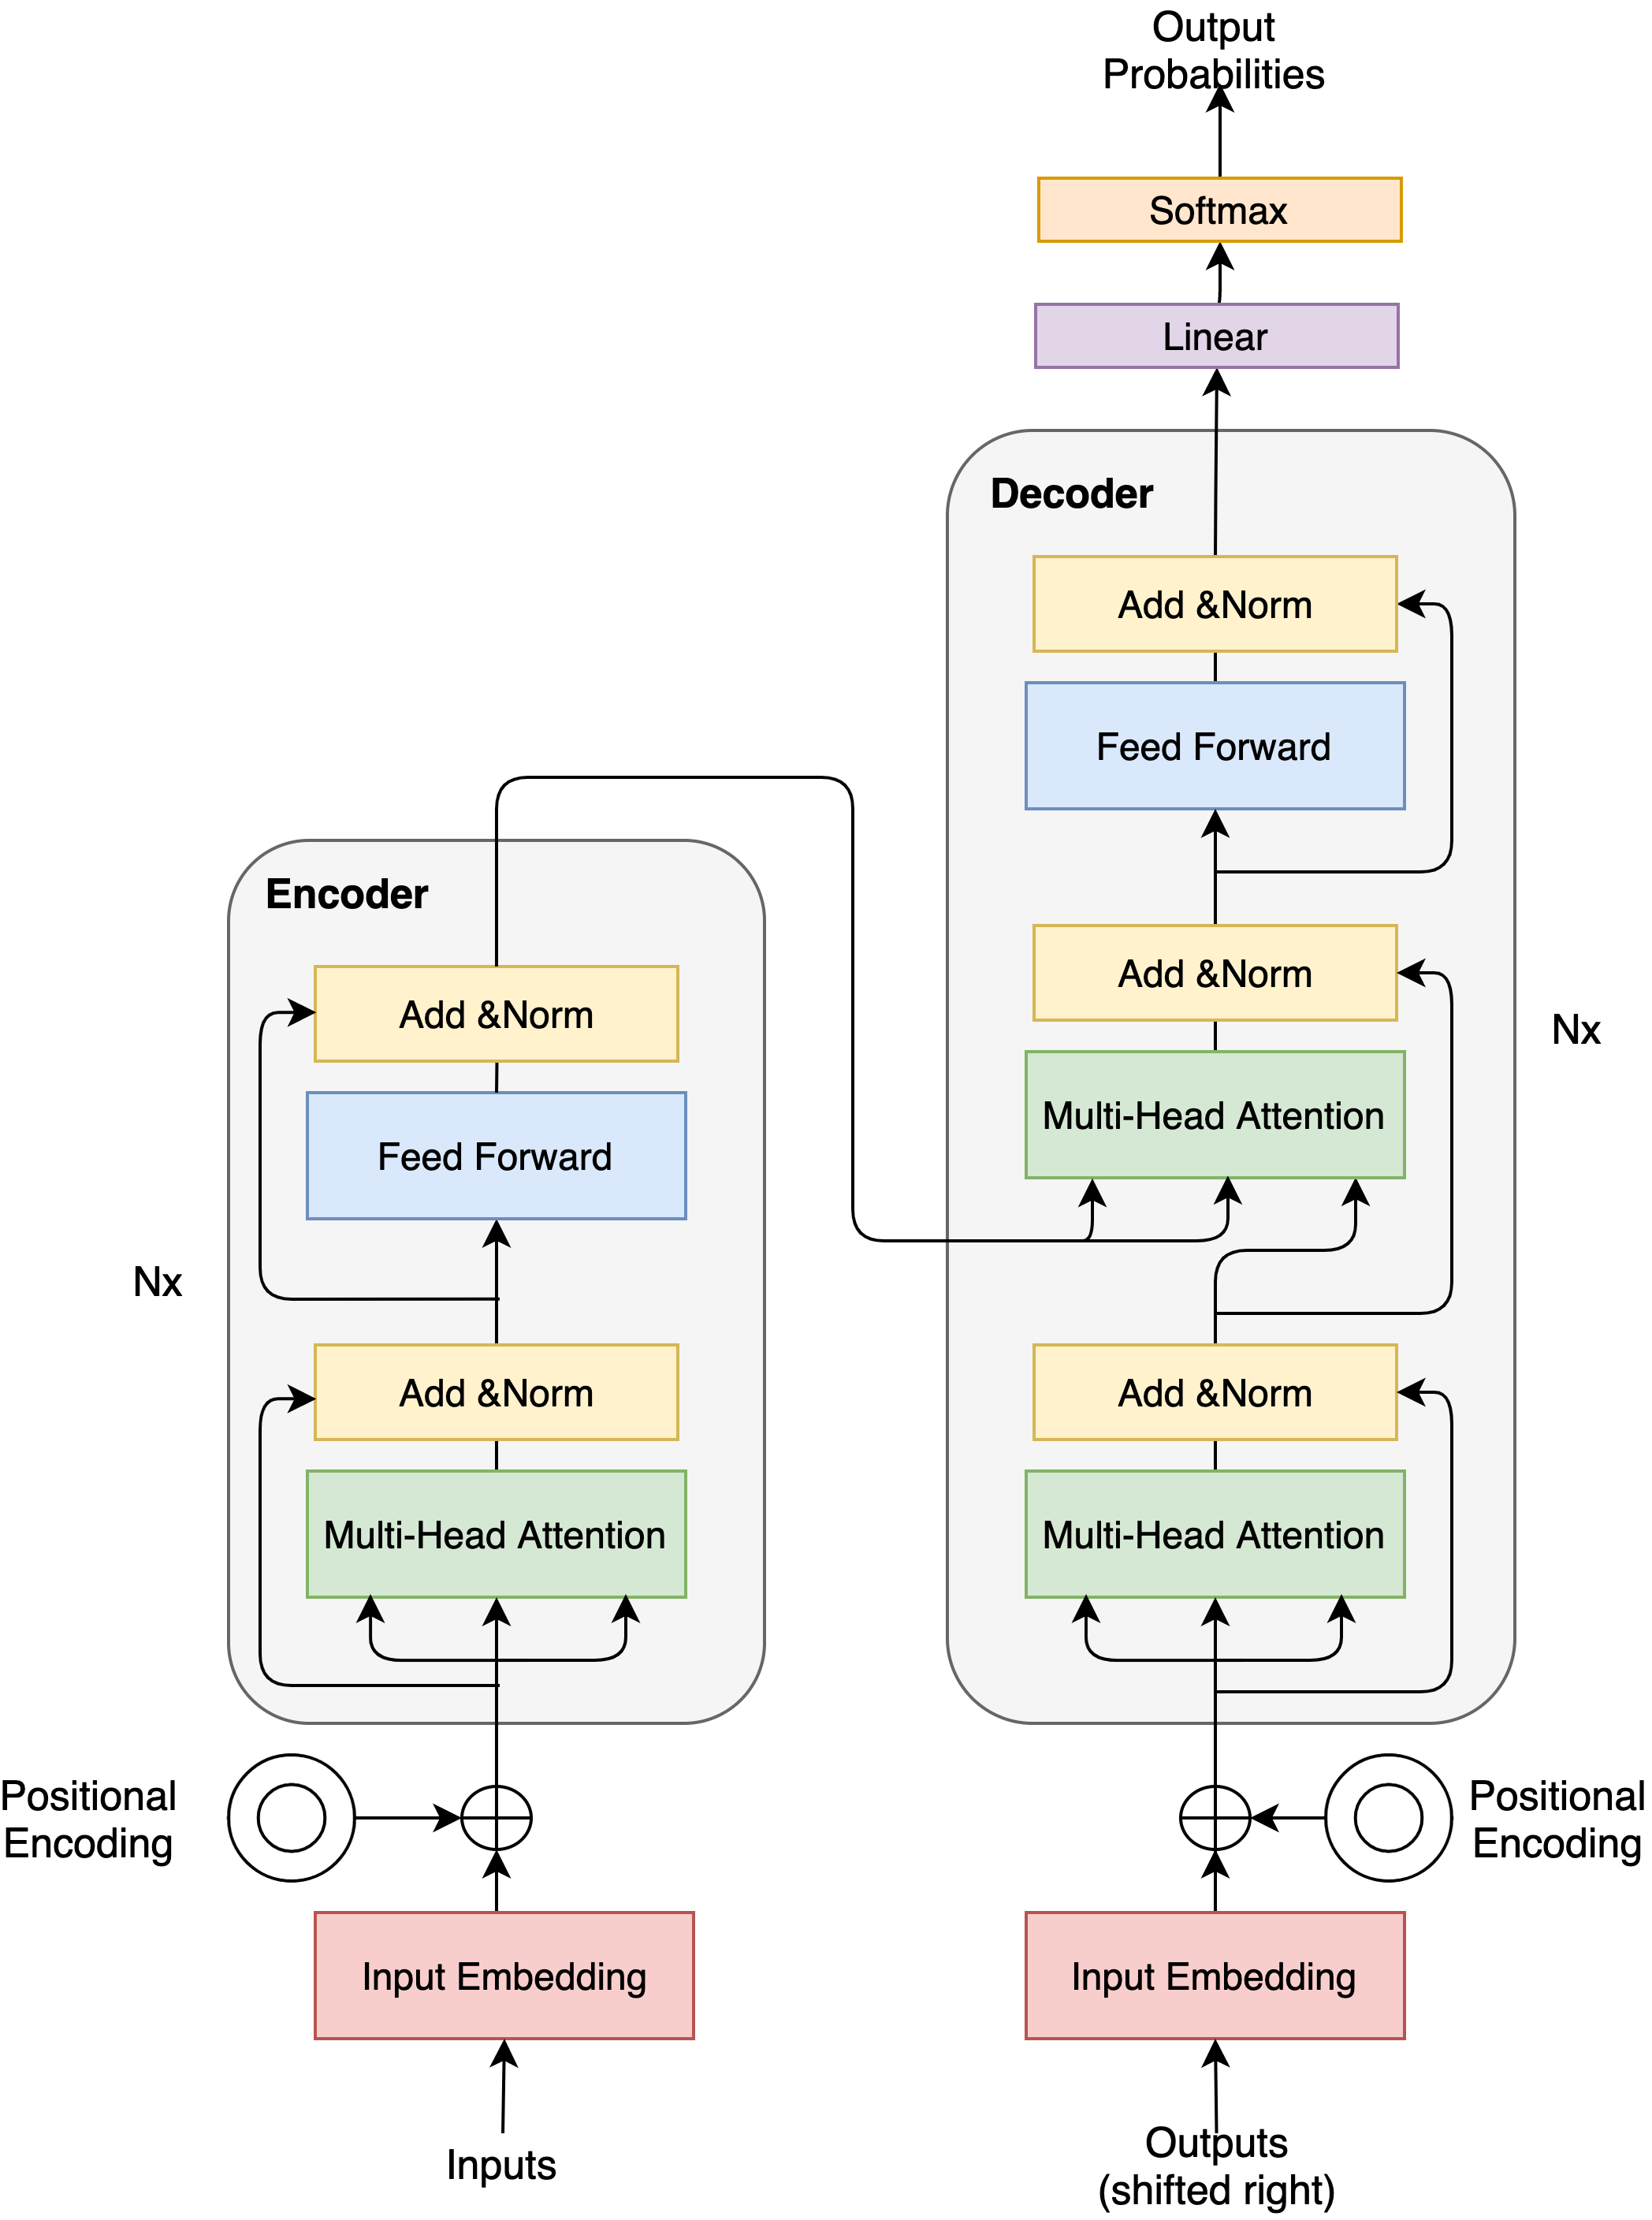
\includegraphics[width = 0.5 \textwidth]{figures/transformer.png}
	\caption[The Transformer - model architecture]
	{ The Transformer - model architecture.~\cite{vaswani2017attention}.}
	\label{fig:transformer}
\end{figure}

\subsection{Self-Attention}
An attention function can be described as mapping a query and a set of key-value pairs to an output, where the query, keys, values, and output are all vectors. The output is computed as a weighted sum of the values, where the weight assigned to each value is computed by a compatibility function of the query with the corresponding key.

From the following table~\ref{tab:complexity_compare}, we can know that self attention has a great improvement for longer sequences. For image data, we can think of it as a longer sequence, and it would be better to optimize it.
\begin{table}[!htbp]
	\resizebox{\textwidth}{15mm}{
	\begin{tabular}{cccc}
		\hline
		Layer Type                  & Complexity per Layer & Sequential Operations & Maximum Path Length \\ \hline
		Self-Attention              & $ O(n2\cdot d)  $           &$  O(1)  $                 & $ O(1)  $               \\
		Recurrent                   & $ O(n2\cdot d) $            & $ O(n)  $                 & $ O(n)  $               \\
		Convolutional               & $O(k\cdot n\cdot d^2)$       & $O(1) $              & $O(log_k(n)$)         \\
		Self-Attention (restricted) & $ O(r\cdot  n \cdot d) $         & $ O(1)  $                 & $ O(n/r)  $             \\ \hline
	\end{tabular}}

\caption[Compare between Self-Attention and Convolutional ]
{ Maximum path lengths, per layer complexity and minimum number of sequential operations for different layer types. n is the sequence length, d is the representation dimension, k is the kernel size of convolutions and r the size of the neighborhood in restricted self-attention. ~\cite{vaswani2017attention}.}
	\label{tab:complexity_compare}
\end{table}

There are three very important vectors in attention, query, key, and value. For self-attention, these three vectors are obtained by multiplying the same vector by different matrices (see in Fig.~\ref{fig:attention}).An attention function can be described as mapping a query and a set of key-value pairs to an output. The input consists of queries and keys of dimension d , and values of dimension d ,softmax function to obtain the weights on the values.


\begin{equation}
	Attention(Q,K,V)=softmax(\frac{QK^T}{\sqrt{d_K}})V
	\label{equ:self_attention}
\end{equation}


\begin{figure}[!htbp]
	\centering
	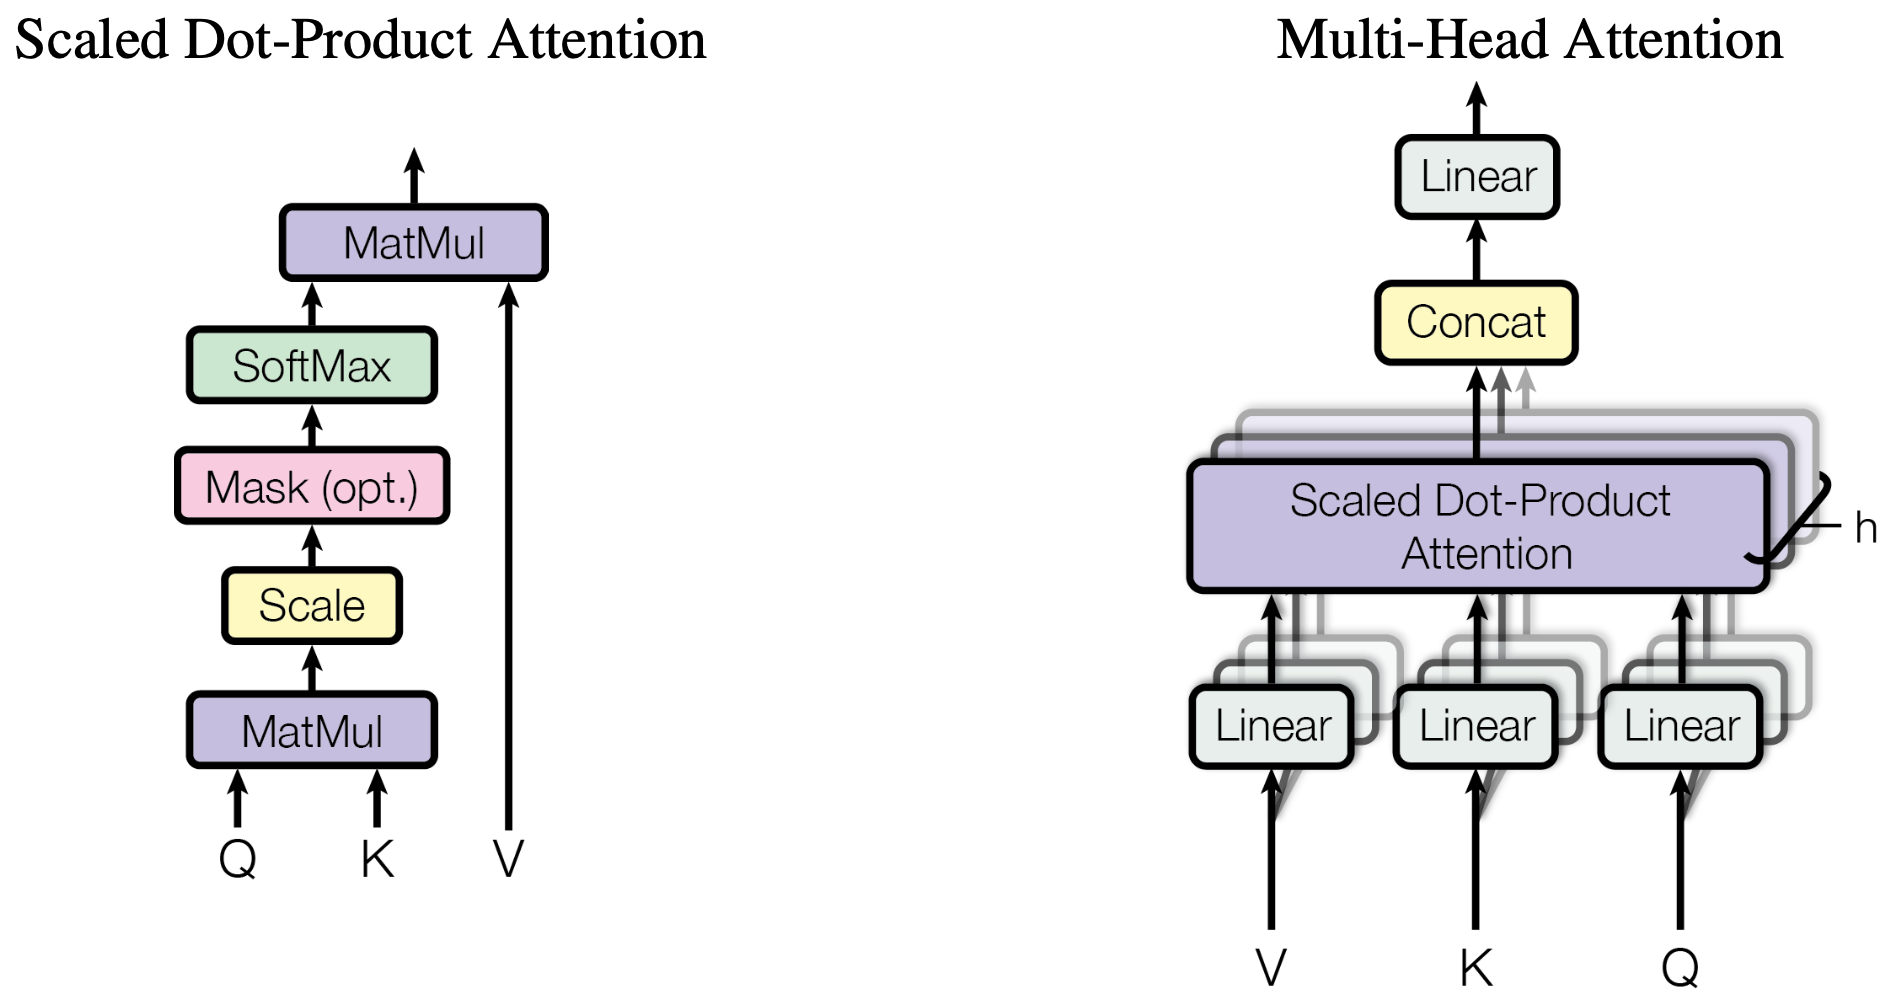
\includegraphics[width = 0.8\textwidth]{figures/attention.png}
	\caption[Scaled Dot-Product Attention and Multi-Head Attention]
	{ (left) Scaled Dot-Product Attention. (right) Multi-Head Attention consists of several attention layers running in parallel. (Image source:~\cite{vaswani2017attention}.)}
	\label{fig:attention}
\end{figure}

\subsection{Multihead Attention}

Multi-head attention allows the model to attend to different representation subspaces at different positions and therefore process richer information. The queries, keys and values are linearly projected h times with different, learned linear projections to dk, dk and dv dimensions respectively. On each of these projections the attention function is computed in parallel, resulting in dv dimensional output values. These are concatenated and projected to obtain the final values, as depicted in Figure 2.3.

\begin{equation}
	\begin{aligned}
MultiHead(Q,K,V) = Concat(head_1,...,head_h)W^O, \\
where \ head_i = Attention(QW_i^Q,KW_i^K,VW_i^V)
\end{aligned}
\end{equation}

\subsection{Positional Encoding}
In the case of RNNs, we feed the words sequentially to the model, each token is aware of how it was ordered. However, multi-head attention computes the output of each item in the sequence independently with no notion of word order. It is inefficient to model the sequence information without any special order or position. To account for the order of the words in the input sequence, the Transformer model adds a vector to each input embedding called Positional Encoding. Positional Encoding from the Transformer model is computed by sine and cosine functions of different frequencies as 
\begin{equation}
	\begin{aligned}
	PE_{(pos,2i)} = sin(pos/10000^{2i/d_{model}}),\\
	PE_{(pos,2i+1)} = cos(pos/10000^{2i/d_{model}})
	\end{aligned}
	\label{equ:position_embedding}
\end{equation}

\subsection{The Overall Model Architecture}
The Transformer model with its encoder and decoder components is illustrated in Figure 11. Both Encoder and Decoder are composed of multiple identical encoders and decoders that can be stacked on top of each other Nx times. The encoder stack and the decoder stack share the same number of Nx.

Encoder: The encoder block is a stack of Nx identical layers. Each layer has a multi-head self-attention mechanism sub-layer followed by a position-wise fully connected feed-forward network sub-layer. There are two on each floor sub-layer, the first is a multi-head self-attention mechanism, and the second is a simple feed-forward network with fully connected locations. The residual structure ~\cite{He_2016_CVPR} (see figure ~\ref{fig:transformer})is used on both sub-layers, and finally layer normalization ~\cite{ba2016layer}. That is, the output of each sub-layer is $LayerNorm(x + Sublayer(x))$, where $Sublayer(x)$ is the function implemented by the sub-layer itself. Since the model does not contain any recurrence and convolution, an embedding must be added to the input so that the model can be used in order of the sequence.

The input received by an encoder is a list of vectors, it will input the list of vectors to the self-attention layer, then pass through the feed-forward neural network layer(FFN), and finally get the output, which is passed to the next encoder. The word at each position passes through the self-attention layer, and each output vector obtained passes through the FFN separately, and the feed-forward neural network through each vector is the same.


Decoder: The decoder block is also a stack of Nx identical layers. In addition to the two sub-layers in each encoder layer, the decoder has an extra Masked Multi-Head Attention sub-layer to avoid this attention sub-layer looking into the future.


\section{Faster R-CNN}

Faster R-CNN~\cite{ren2016faster} is an advanced network for object detection and the cornerstone for the visual relationship detection models. Compared with other object detection models, Faster R-CNN performs well on localizing and classifying the objects in images. Therefore, it is used as the backbone of object detection in many works about visual relationship detection~\cite{zellers2018neural}. Faster R-CNN contains four parts: convolutional layers, region proposal network (RPN), ROI pooling and classifier. In visual relationship detection, the first three parts are utilized to extract the feature map and localize the bounding boxes of objects. The classifier of Faster R-CNN is generally replaced by the advanced model which is designed for visual relationship detection. The structure of Faster R-CNN is illustrated in Fig.~\ref{fig:fasterrcnn}.

\begin{figure}[!htbp]
	\centering
	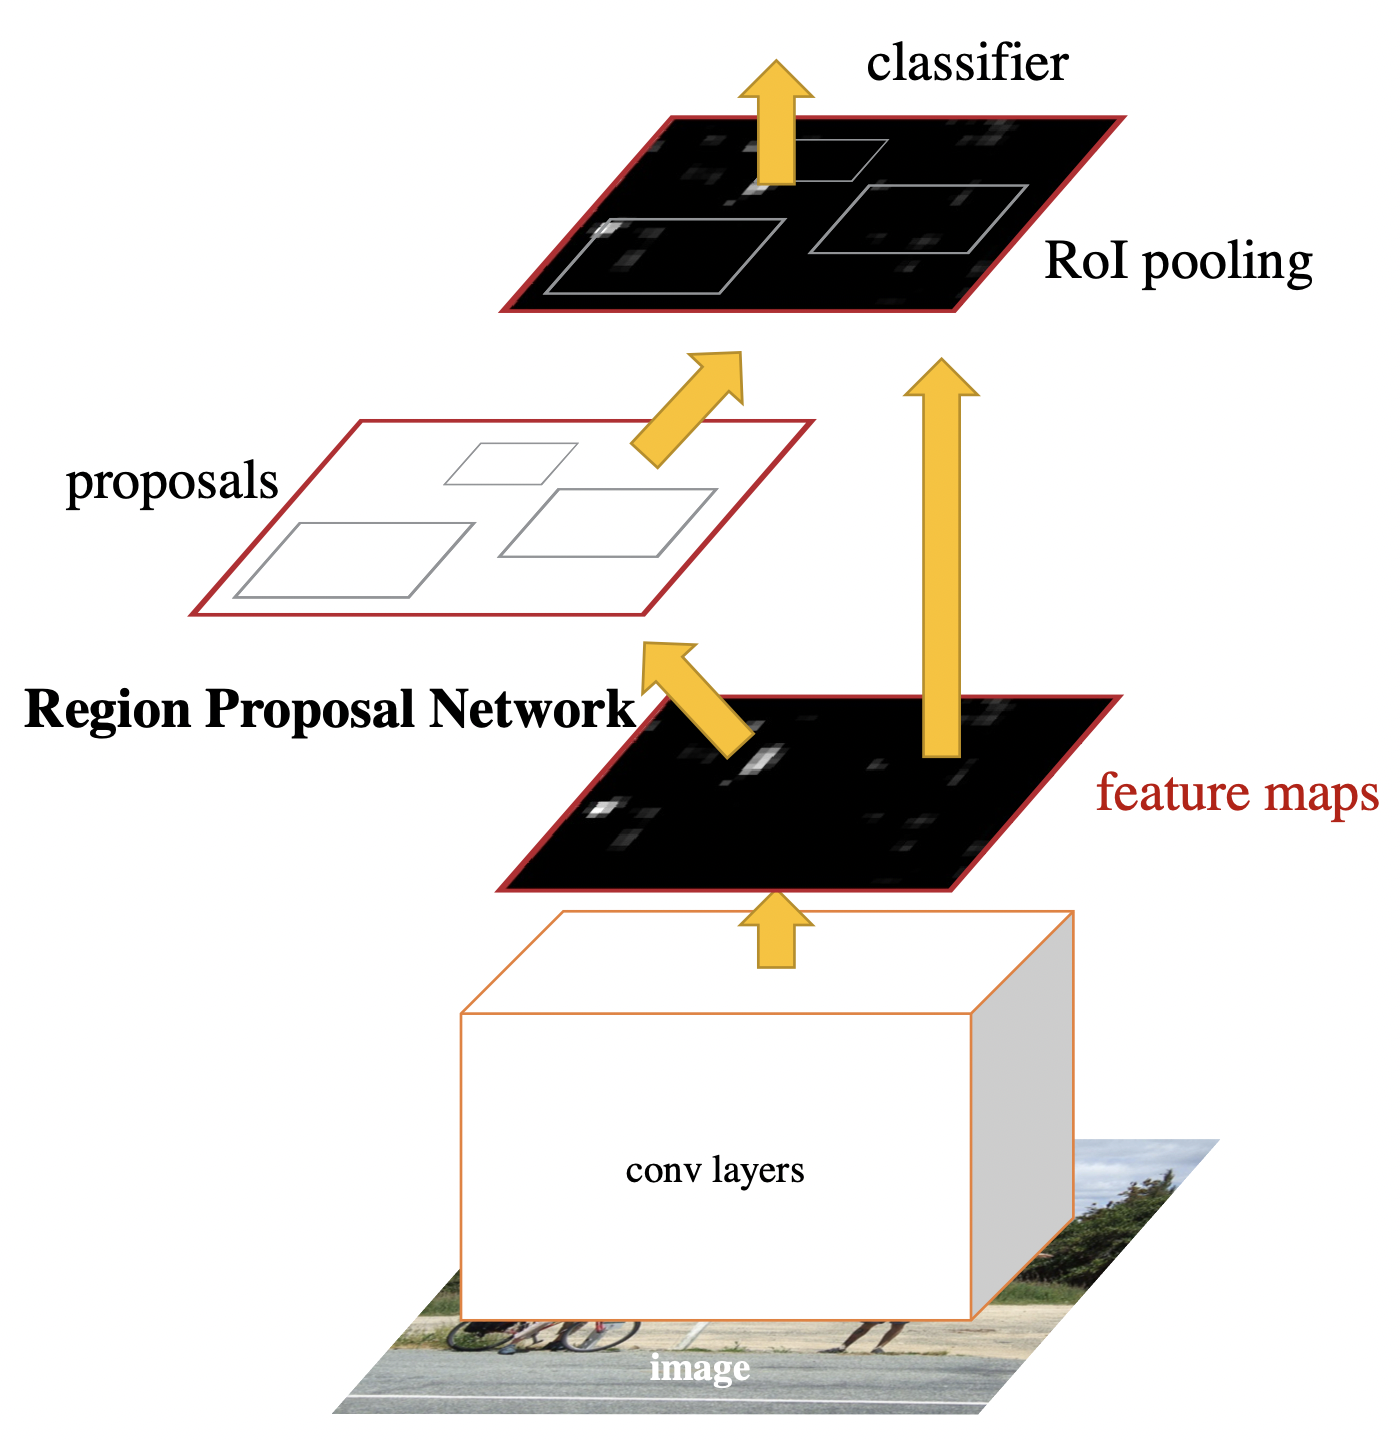
\includegraphics[width = 0.7\textwidth]{figures/fasterrcnn.png}
	\caption[The architecture of Faster R-CNN]
	{ The architecture of Faster R-CNN.}
	\label{fig:fasterrcnn}
\end{figure}

The following are the key steps of Faster RCNN:
\begin{itemize}
	\item \textbf{Conv layers.} As a CNN network target detection method, Faster R-CNN first uses a set of basic conv, relu and pooling layers to extract image feature maps. The feature maps are shared for the subsequent RPN layer and fully connected layer.
	\item \textbf{Region Proposal Networks.} The RPN network is used to generate region proposals. This layer judges that anchors belong to foreground or background through softmax, and then uses bounding box regression to correct anchors to obtain accurate proposals.
	\item \textbf{Roi Pooling. }This layer collects the input feature maps and proposals, extracts the proposal feature maps after synthesizing the information, and sends them to the subsequent fully connected layer to determine the target category.
	\item \textbf{Classification}. Use proposal feature maps to calculate the category of the proposal, and again bounding box regression to obtain the final precise position of the bounding box.
\end{itemize}

\subsection{VGG16}

VGG16 is a convolutional neural network model proposed by K. Simonyan and A. Zisserman from the University of Oxford in the paper ``Very Deep Convolutional Networks for Large-Scale Image Recognition''~\cite{simonyan2015deep}. The model achieves 92.7\% top-5 test accuracy in ImageNet~\cite{ILSVRC15}, which is a dataset of over 14 million images belonging to 1000 classes.

The structure of VGG16 is shown in Fig.~\ref{fig:vgg16}.The input to cov1 layer is of fixed size 224 x 224 RGB image. The image is passed through a stack of convolutional (conv.) layers, where the filters were used with a very small receptive field: 3x3 (which is the smallest size to capture the notion of left/right, up/down, center). In one of the configurations, it also utilizes 1x1 convolution filters, which can be seen as a linear transformation of the input channels (followed by non-linearity). The convolution stride is fixed to 1 pixel; the spatial padding of conv. layer input is such that the spatial resolution is preserved after convolution, i.e. the padding is 1-pixel for 3x3 conv. layers. Spatial pooling is carried out by five max-pooling layers, which follow some of the conv.  layers (not all the conv. layers are followed by max-pooling). Max-pooling is performed over a 2x2 pixel window, with stride 2.

Three Fully-Connected (FC) layers follow a stack of convolutional layers (which has a different depth in different architectures): the first two have 4096 channels each, the third performs 1000-way ILSVRC classification and thus contains 1000 channels (one for each class). The final layer is the soft-max layer. The configuration of the fully connected layers is the same in all networks.

All hidden layers are equipped with the rectification (ReLU) non-linearity. It is also noted that none of the networks (except for one) contain Local Response Normalisation (LRN), such normalization does not improve the performance on the ILSVRC dataset, but leads to increased memory consumption and computation time.


\begin{figure}[!htbp]
	\centering
	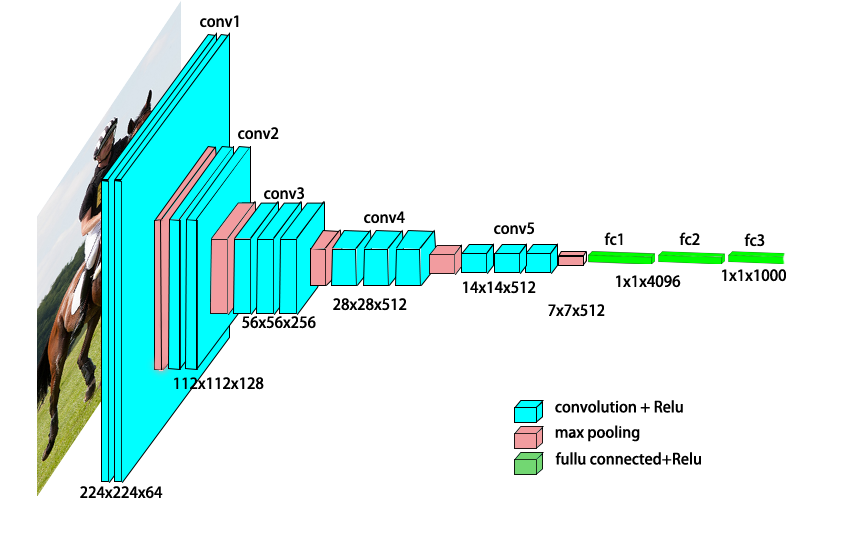
\includegraphics[width=0.8\linewidth]{figures/vgg16}
	\caption[The Architecture of VGG-16]{The Architecture of VGG-16.}
	\label{fig:vgg16}
\end{figure}

The advantages of VGG:
\begin{itemize}
	\item The structure of VGGNet is very simple, the entire network uses the same size of the convolution kernel size (3x3) and maximum pooling size (2x2).
	\item The combination of several small filter (3x3) convolutional layers is better than a large filter (5x5 or 7x7) convolutional layer.
	\item It is verified that performance can be improved by continuously deepening the network structure.
\end{itemize}

The disadvantages of VGG:

\begin{itemize}
	\item VGG consumes more computing resources and uses more parameters, resulting in more memory usage. Most of the parameters are from the first fully connected layer. VGG has 3 fully connected layers!
\end{itemize}



\label{sec:roialign}
\subsection{ROI Align}
ROI Align is a regional feature aggregation method proposed in the Mask-RCNN~\cite{he2018mask} paper, which solves the problem of regional mis-alignment caused by two quantizations in the ROI Pooling operation. Experiments show that replacing ROI Pooling with ROI Align in the detection task can improve the accuracy of the detection model.

\begin{figure}[!htbp]
	\centering
	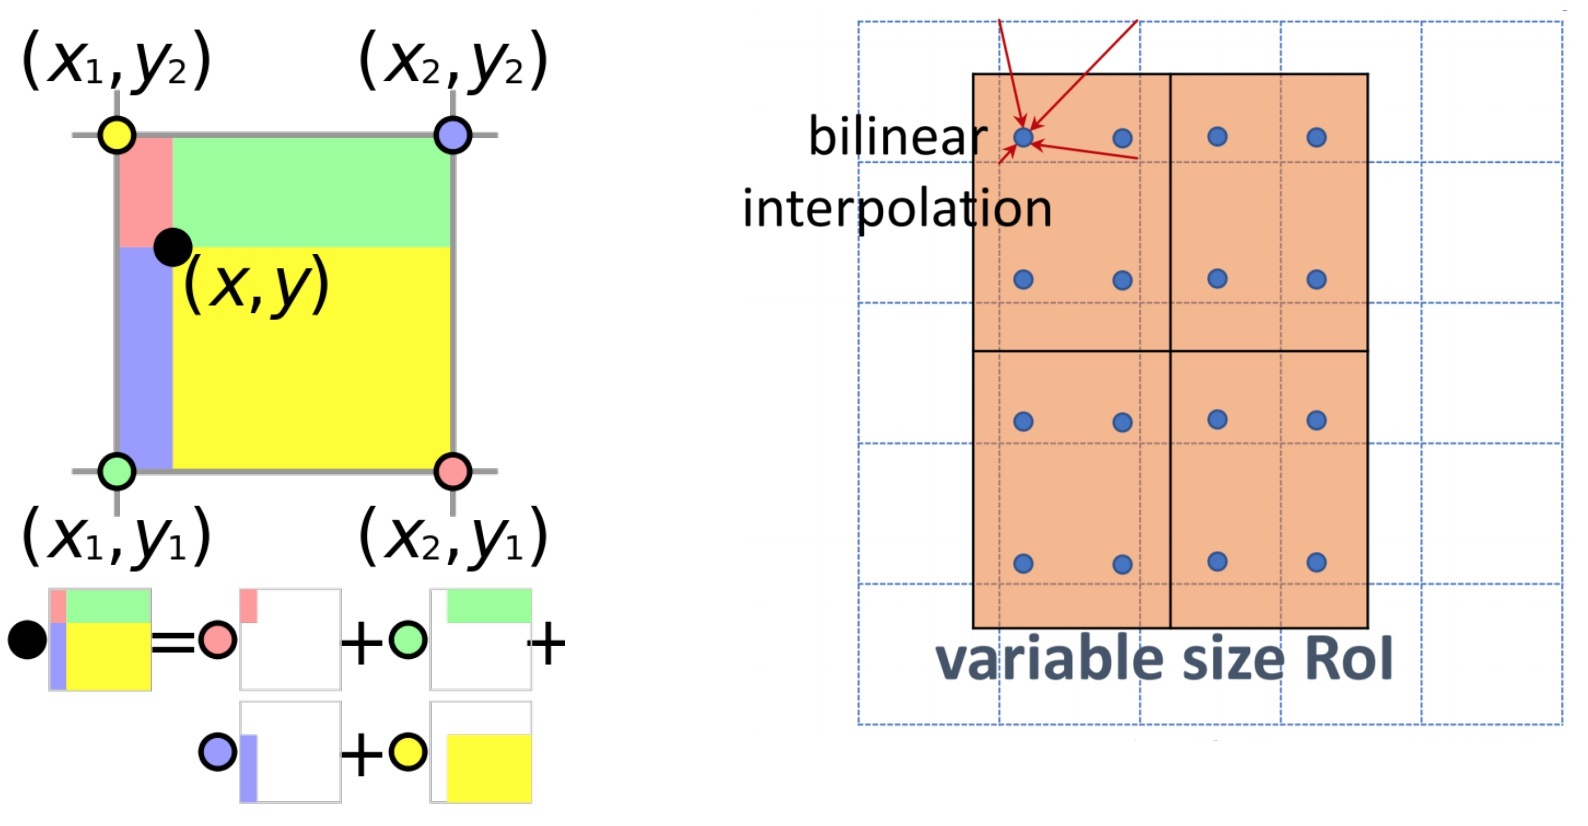
\includegraphics[width=1\linewidth]{figures/roi_align}
	\caption[Bilinear interpolation for ROI Align]{Bilinear interpolation for ROI Align.}
	\label{fig:roialign}
\end{figure}

ROI Align does not need to perform rounding operations like ROI pooling. If the decimal number is calculated, that is, it does not fall on the real pixel, then use the nearest pixel to perform bilinear interpolation on this virtual pixel to get this `pixel'  value.The step are processed as follow:

\begin{enumerate}[1.]
	\item Divide the bbox area into equal parts according to the size required by the output. It is likely that the vertices will not fall on the real pixels after the equal division.
	\item If the vertices do not fall on the real pixel points after equal division, then take a fixed 4 points in each bin, which is the blue point on the right side of Figure~\ref{fig:roialign}.
	\item For each blue point, the value of the 4 nearest real pixel points is weighted (bilinear interpolation) to obtain the value of this blue point
	\item  4 new values are calculated in a bin, and max is selected from these new values as the output value of this bin Therefore we use bilinear interpolation to predict its value.
	\item Get the final 2x2 output.
\end{enumerate}

\section{End-to-End Object Detection with Transformers}
The DETR discards the traditional Faster R-CNN ROI-based object detection method, and uses Transformer and its proposed bipartite matching to achieve position-independent and unique bounding box for each object, thus eliminating the need for Anchor and NMS. With a very simple architecture, it achieves an accuracy comparable to or even surpassing Faster R-CNN. While being able to do object detection, the model also has better migration capabilities. In the original paper, the panoramic segmentation was achieved through the Transformer's Attention mechanism. 

\begin{figure}[!htbp]
	\centering
	\includegraphics[width = 1 \textwidth]{figures/DETR.png}
	\caption[The framework of DETR model]
	{ The framework of DETR model. Figure obtained from ~\cite{carion2020end}}
	\label{fig:detr}
\end{figure}

The network structure of DETR is very simple (see in Fig.~\ref{fig:detr}.). It is divided into three parts: the first part is a traditional CNN to extract image features to higher dimensions. The second part is a Transformer Encoder and Decoder to extract the object features. Finally, the Bipartite matching loss is used to Train the network. 

\subsection{Transformer Encoder}

As shown on the left side of the Fig.~\ref{fig:detr}, the DETR first enter the picture $ x_{img} \in  \mathbb{R} ^{3\times H_0\times W_0} $. After processing by CNN backbone, output feature map $ f \in \mathbb{R} ^{C\times H\times W } $, where $ C = 2048, H=\frac{H_0}{32}, W=\frac{W_0}{32}  $. Then add the feature map and position encoding, and input them into the Transformer Encoder for processing, and obtain the image embedding for input to the Transformer Decoder. Since the input of Transformer is serialized data, the feature map output by backbone is further processed and converted into serialized data. 
As shown on the left side of the figure, the result of detr's transformer encoder is the same as the traditional transformer structure, except that the input is replaced with image features.

\subsection{Transformer Decoder}

detr passes the predicted target sequence obtained by the Transformer encoder through the Transformer decoder shown in the right half of Figure~\ref{fig:detrtr}, and decodes it in parallel to obtain the output sequence (rather than outputting it element by element like machine translation). Different from the traditional autogreesive mechanism, each layer can decode N targets. Due to the position invariance of the decoder, that is, the result of switching the input order is unchanged, in addition to the information of each pixel itself, the position information is also very important, so these N targets The input embedding must be different to produce different results, so learn the method in NLP, add positional encoding and add it for each layer.

In addition, a fixed-size learnable object query is designed in DETR, which defines an embedding layer with a size of $ [100, 256] $, and uses its parameters as the object query. While training the network, the object query is also training, so that the most suitable query tensor is obtained and fixed.

\begin{figure}
	\centering
	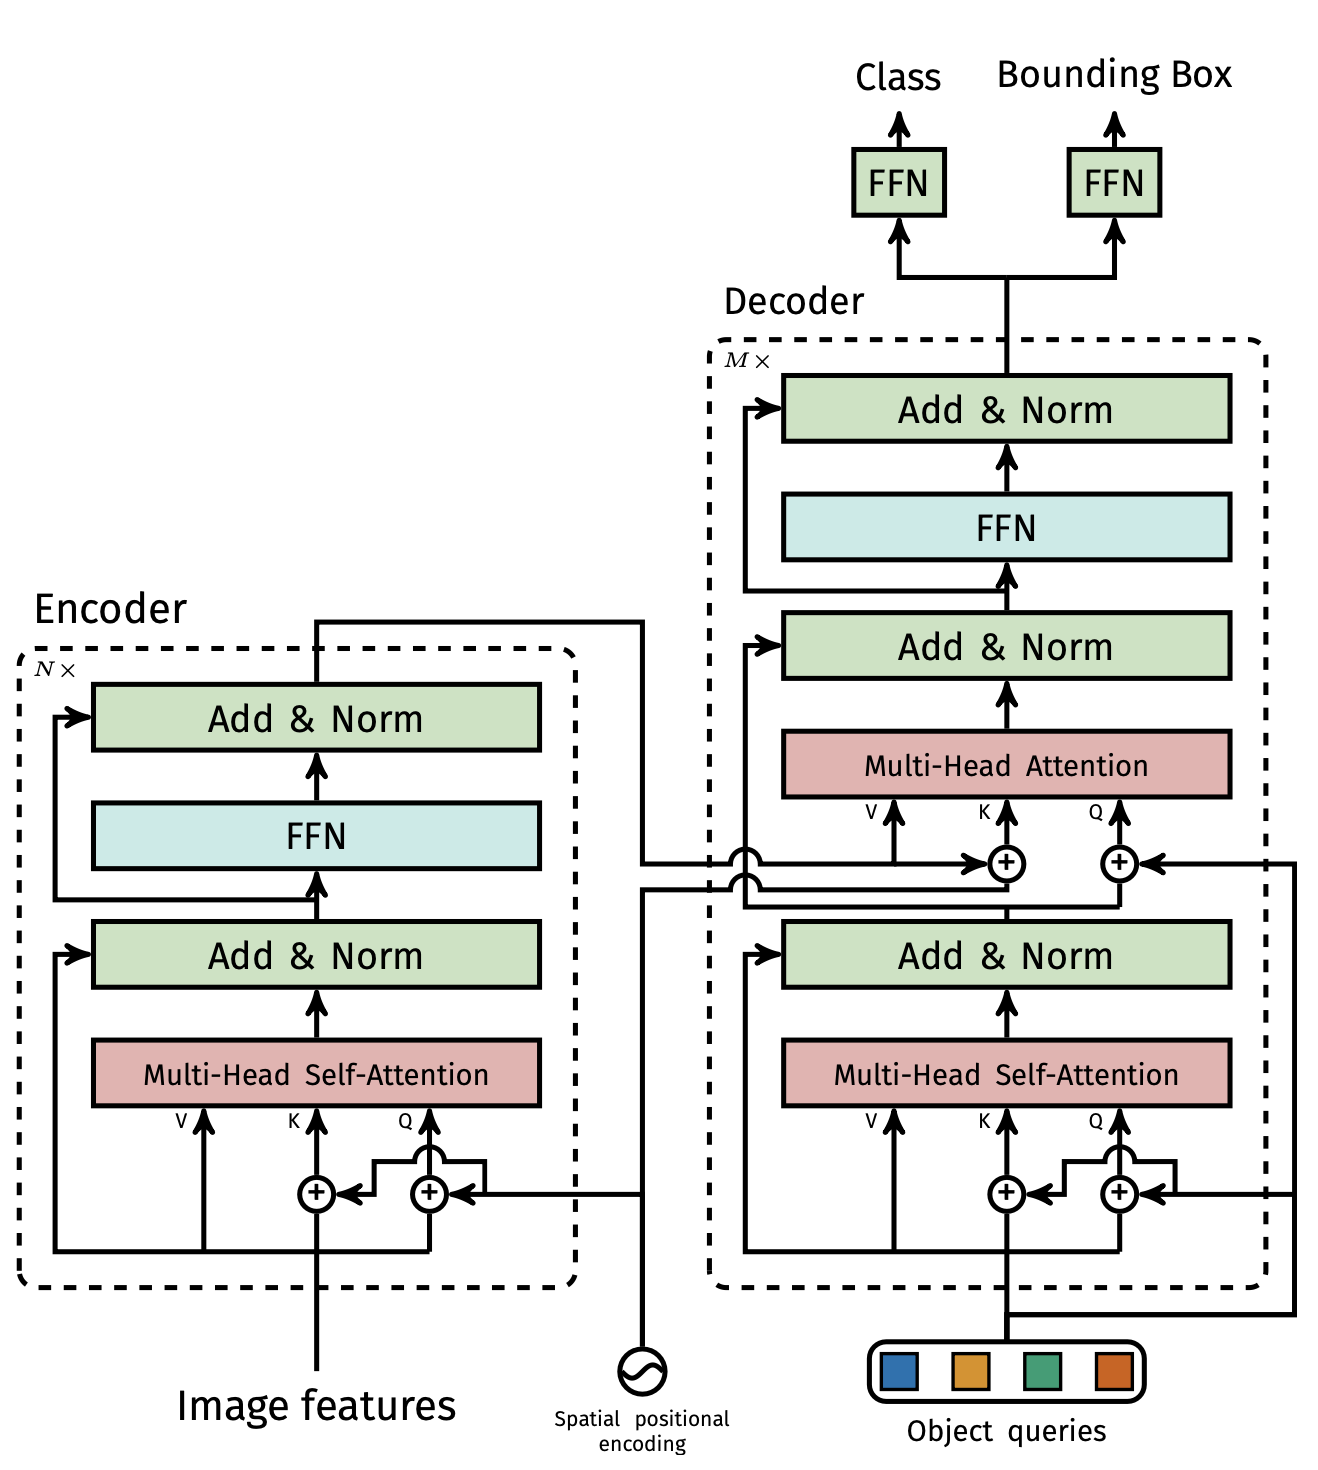
\includegraphics[width=0.7\linewidth]{figures/detr_tr}
	\caption[Architecture of DETR's transformer]{Architecture of DETR's transformer, figture obtained from ~\cite{carion2020end}.}
	\label{fig:detrtr}
\end{figure}


\subsection{Bipartite matching loss}

Previously, the detector used the anchor and ground truth IoU to determine the positive and negative samples,  while DETR used bipartite matching loss to determine the positive and negative samples. 

\begin{equation}
	\hat{\sigma}=\underset{\sigma \in \mathfrak{G}_{N}}{\arg \min } \sum_{i}^{N} \mathcal{L}_{\text {match }}\left(y_{i}, \hat{y}_{\sigma(i)}\right)
\end{equation}

Where $ \mathcal{L}_{\text {match }} $ is the pair-wise matching cost between ground true and predicted bounding boxes. Through one-by-one pairing, there is no need to adopt traditional NMS, because a bounding box can only be matched with a ground true, which will inevitably introduce loss. The algorithm implementation uses the Hungarian algorithm.

\subsubsection{Hungarian matching }

Hungarian matching is binary matching using the Hungarian algorithm, it is also a maximum matching. The purpose of maximum matching is to match an edge for each node as much as possible, and the match with the largest number of edges is the maximum match. Usually, in binary matching, each node can only match one edge.

\begin{figure}
	\centering
	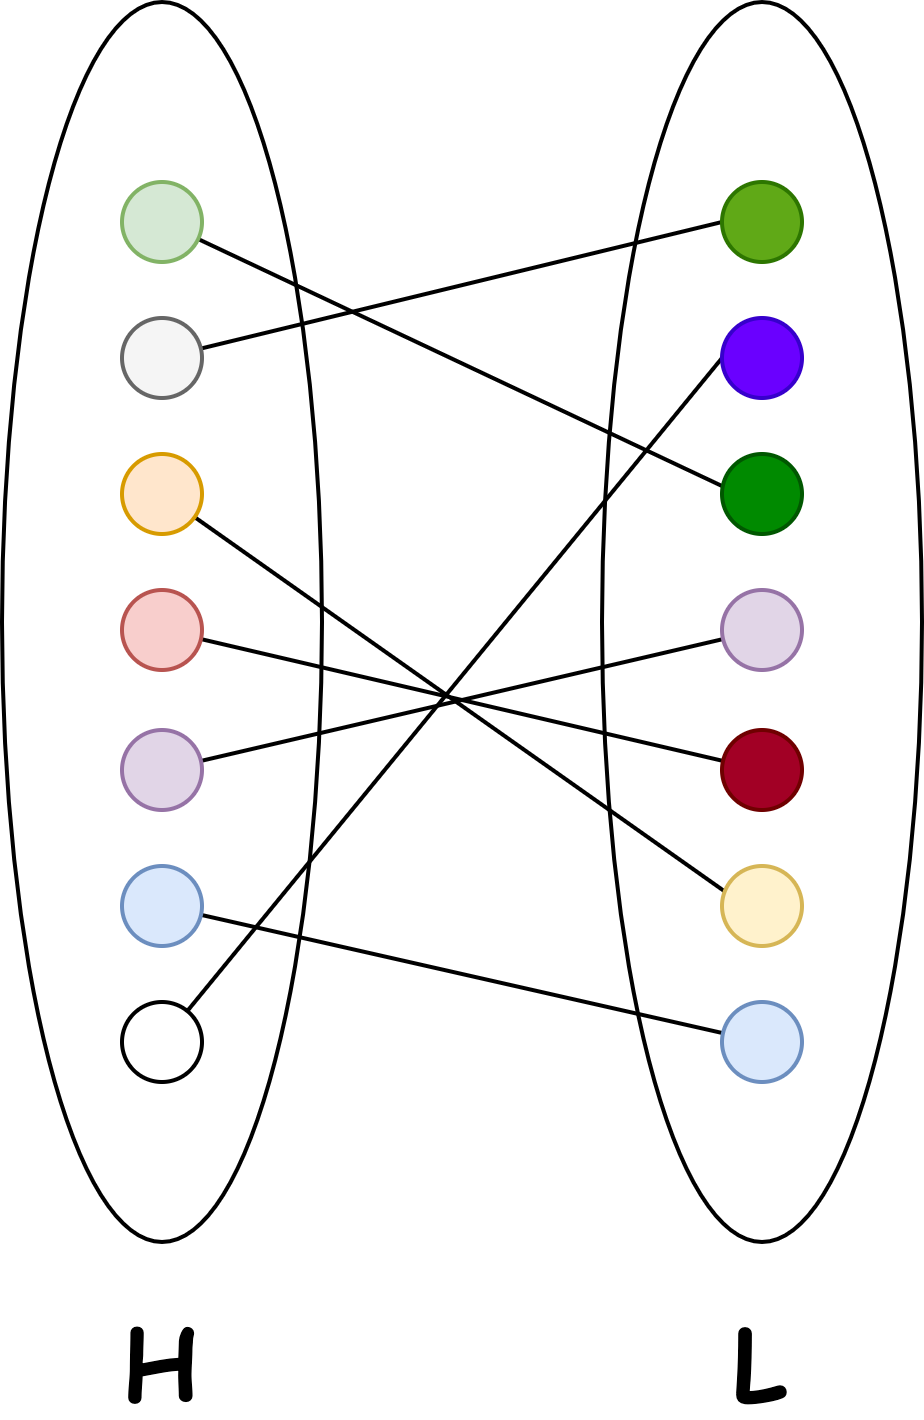
\includegraphics[width=0.3\linewidth]{figures/matcher}
	\caption[Bipartite matching loss]{Bipartite matching loss.}
	\label{fig:matcher}
\end{figure}

The basic steps of the Hungarian algorithm are as follows:
\begin{enumerate}[1.]
	\item Subtract the smallest entry in each row from all the other entries in the row. This will make the smallest entry in the row now equal to 0.
	\item Subtract the smallest entry in each column from all the other entries in the column. This will make the smallest entry in the column now equal to 0
	\item Draw lines through the row and columns that have the 0 entries such that the fewest lines possible are drawn.
	\item  If there are nn lines drawn, an optimal assignment of zeros is possible and the algorithm is finished. If the number of lines is less than nn, then the optimal number of zeroes is not yet reached, then go to the next step.
	\item Find the smallest entry not covered by any line. Subtract this entry from each row that is not  crossed out, and then add it to each column that is crossed out. Then, go back to Step 3.
\end{enumerate}

The loss calculation in DETR includes classification loss and box regression loss:

\begin{equation}
	\mathcal{L}_{\text {Hungarian }}(y, \hat{y})=\sum_{i=1}^{N}\left[-\log \hat{p}_{\hat{\sigma}(i)}\left(c_{i}\right)+\mathbb{1}_{\left\{c_{i} \neq \varnothing\right\}} \mathcal{L}_{\text {box }}\left(b_{i}, \hat{b}_{\hat{\sigma}}(i)\right)\right]
\end{equation}

The regression loss $ \mathcal{L}_{\text {box }} $ does not calculate \textit{no object}, and the regression loss $ \mathcal{L}_{\text {box }} $ includes $  L_1 $ loss and GIoU loss.

\subsubsection{IoU and GIoU}

IoU is what we call cross-union ratio, which is the most commonly used index in target detection, in the anchor-based method. The function is not only used to determine the positive sample and the negative sample, but also can be used to evaluate the distance between the predict box and the ground-truth.

$$
I o U=\frac{|A \cap B|}{|A \cup B|}
$$

GIoU was proposed by Hamid et al.~\cite{rezatofighi2019generalized}, since IoU is the concept of ratio, it is not sensitive to the scale of the target object. However, the BBox regression loss (MSE loss, $ l_1 $ smooth loss, etc.) optimization and IoU optimization in the detection task are not completely equivalent, and the Ln norm is also sensitive to the scale of the object, and IoU cannot directly optimize the part that does not overlap.
$$
G I o U=I o U-\frac{\left|A_{c}-U\right|}{\left|A_{c}\right|}
$$

The above formula means: first calculate the area of the smallest closed area of the two boxes, that is, the area of the smallest box that contains both the predicted box and the ground truth box, then calculate the IoU, and then calculate the area of the closed area that does not belong to the two boxes. The area accounts for the proportion of the closure area, and finally IoU is used to subtract this proportion to get GIoU.


\subsection{Visualizing attention}
As shown in Figure ~\ref{fig:detrattentionmap}, we can clearly see what detr pays more attention to a picture through the attention map, and the focus of each of his object features can be reflected in the attention map. Even DETR has good scalability and can be used for image segmentation.

\begin{figure}
	\centering
	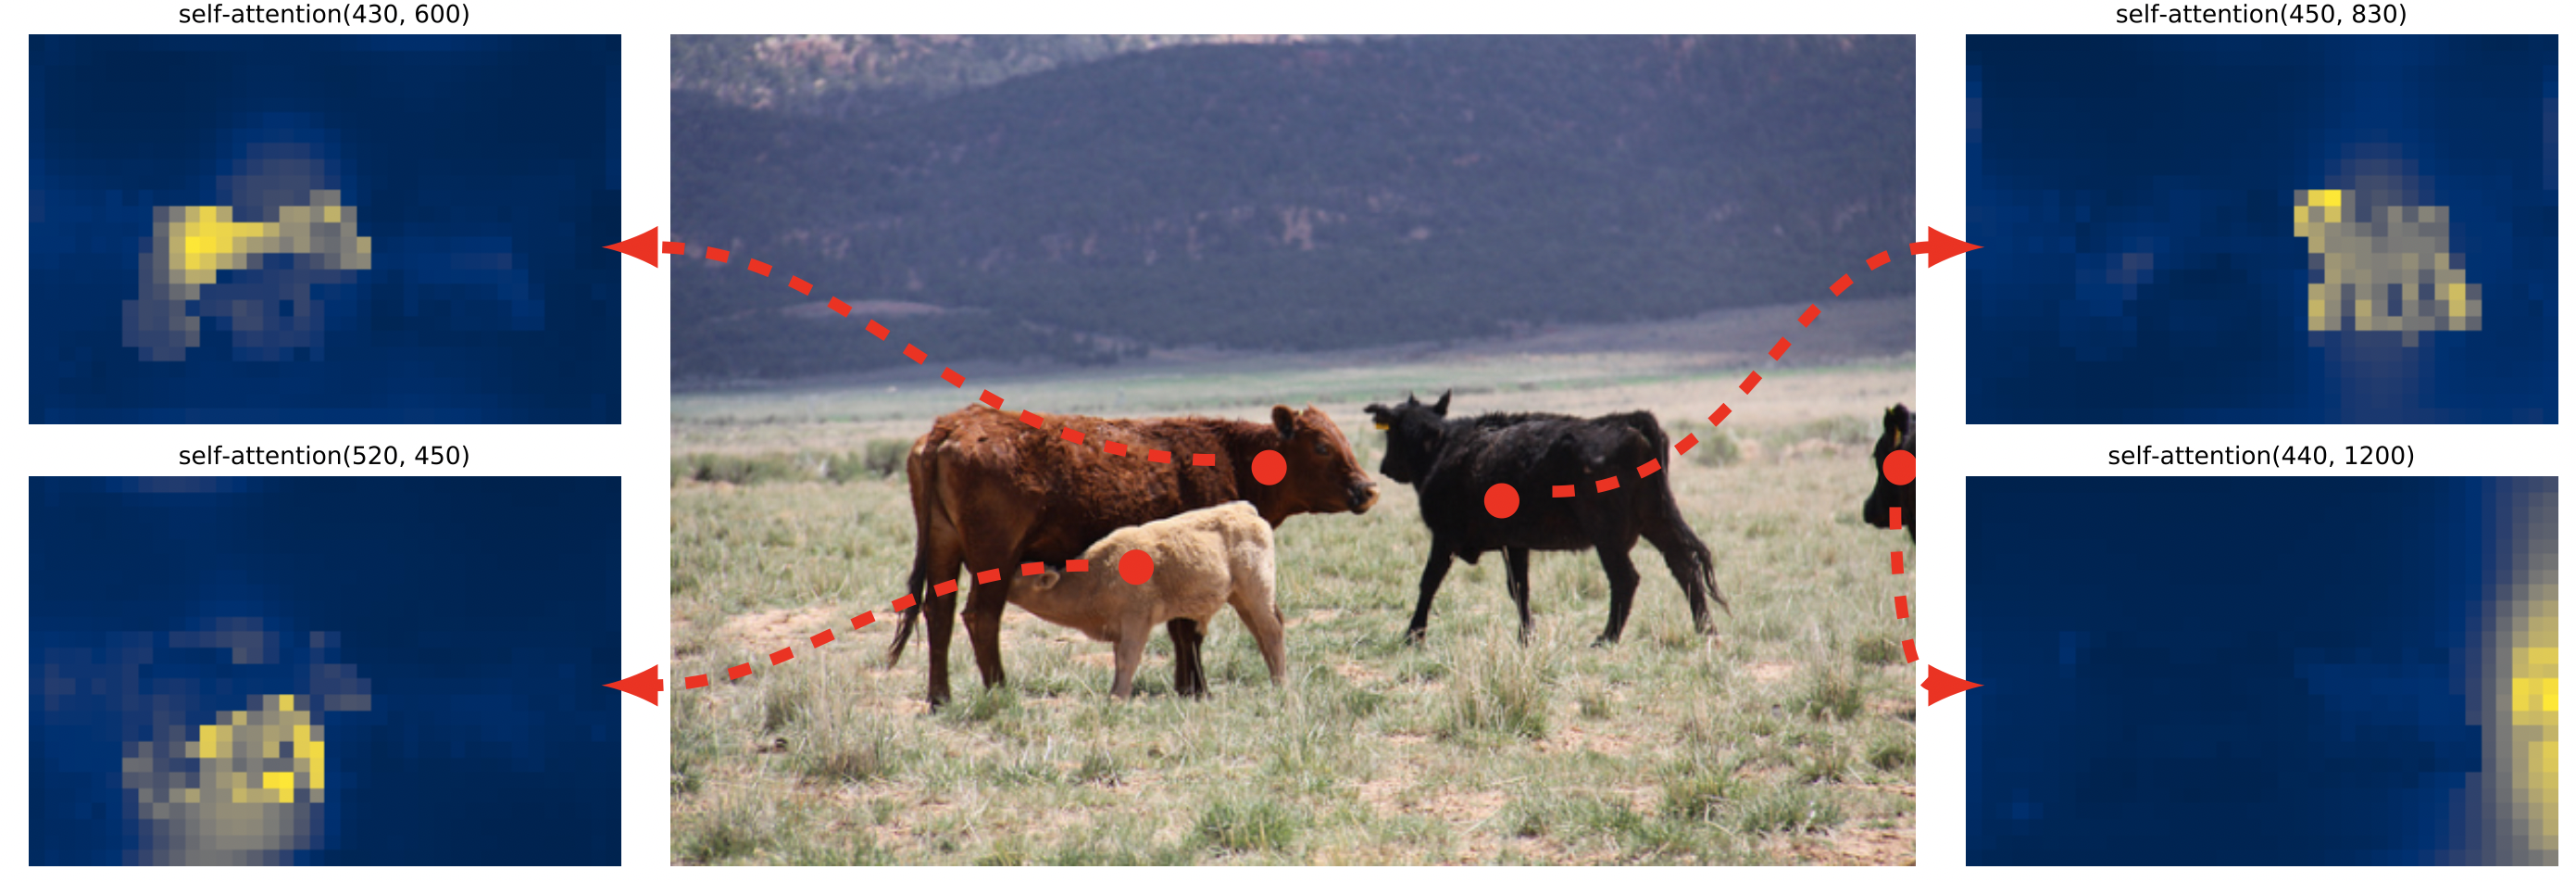
\includegraphics[width=1\linewidth]{figures/detr_attention_map}
	\caption[The attention map of the model DETR]{The attention map of the model DETR. The Encoder Self-Attention is able to separate individual instances, and it can be well visualized in the attention map. mage source from Carion et al.~\cite{carion2020end} page 11.}
	\label{fig:detrattentionmap}
\end{figure}




\section{Ranking Loss}

Different from Cross-Entropy Loss ~\cite{Categorical_Loss} or Mean Square Error Loss(MSE) ~\cite{CHRISTOFFERSEN2004291}, their goal is to characterize the difference between the output of the model and the actual output. But ranking loss is actually a kind of metric learning, the relative distance they learn does not care about the actual value. Because there are different names in different scenes, including Contrastive Loss, Margin Loss, Hinge Loss or Triplet Loss.

Ranking loss is widely used, including two categories, such as face recognition, which is a person or not a person.

\begin{figure}[!htbp]
	\centering
	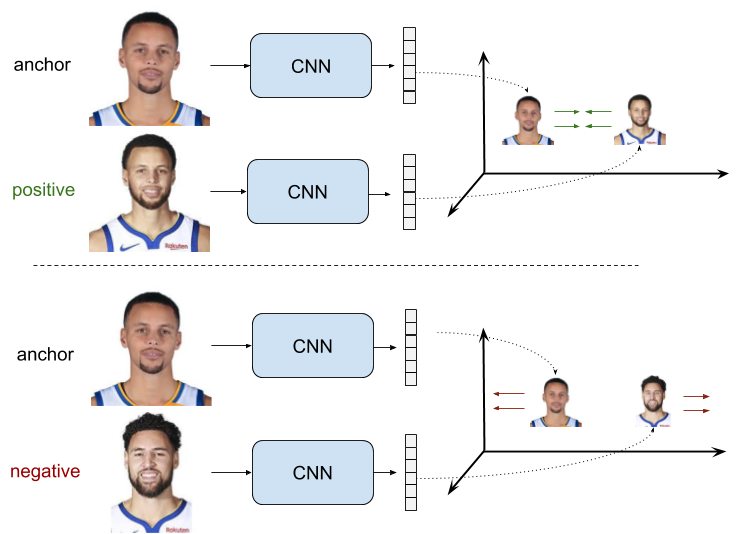
\includegraphics[width = 0.8\textwidth]{figures/pairwise_ranking_loss_faces.png}
	\caption[Example of a pairwise ranking loss ]
	{ Example of a pairwise ranking loss setup to train a net for image face verification. In this setup, the weights of the CNNs are shared. We call it siamese nets. But a pairwise ranking loss can be used in other setups, or with other nets.(Image source:~\cite{triplet_loss_em}.)}
	\label{fig:pairwise_ranking_loss}
\end{figure}


The objective is to learn representations with a small distance $d$ between them for positive pairs, and greater distance than some margin value $m$ for negative pairs. Pairwise Ranking Loss forces representations to have $0$ distance for positive pairs, and a distance greater than a margin for negative pairs. Being $r_a$ and $r_p$the samples representations and $d$ a distance function, we can write:

\begin{equation}
L=\begin{cases}
	d(r_a,r_p) & if \qquad positive\ pair \\
	max(0,m-d(r_a,r_p)) & if \qquad negative\  pair
\end{cases}
\end{equation}

Suppose $r_0,r_1 $ is used to represent the representation of the two elements of the sample, $y$is a two-valued value, when the input is a negative sample pair, it is 0, when a positive sample pair is input, it is 1, and the distance $d$ is Euclidean distance , We can have the final loss function expression:

\begin{equation}
L(r_0,r_1,y)=y\left || r_0-r_1 \right || + (1-y)max(0,m-\left || r_0-r_1 \right ||)
\end{equation}

This setup outperforms the former by using triplets of training data samples, instead of pairs. The triplets are formed by an anchor sample $x_a$, a positive sample $x_p$ and a negative sample $x_n$. The objective is that the distance between the anchor sample and the negative sample representations $d(r_a,r_n)$ is greater (and bigger than a margin $m$) than the distance between the anchor and positive representations $d(r_a,r_p)$. With the same notation, we can write:

\begin{equation}
L(r_a,r_p,r_n)=max(0,m+d(r_a,r_p)-d(r_a,r_p))
\label{equ:ranking_loss}
\end{equation}

\begin{figure}[!htbp]
	\centering
	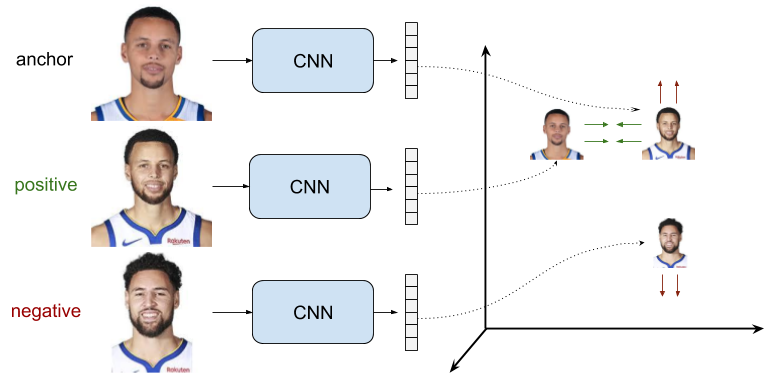
\includegraphics[width = 0.8\textwidth]{figures/triplet_loss_faces.png}
	\caption[Example of a triplet ranking loss ]
	{ Example of a triplet ranking loss setup to train a net for image face verification. In this setup, the weights of the CNNs are shared. We call it triple nets. (Image source:~\cite{triplet_loss_em}.)}
	\label{fig:triplet_ranking_loss}
\end{figure}


\section{Word Representation}

Same as location information, semantic information also helps a lot for understanding relations. The basic encoding method is one hot code. 

One-hot representation is another natural approach to represent words, which assigns a unique index to each word. It is also not good enough to represent words with one-hot representation. First, one-hot representation could not capture the semantic relatedness among words. Second, one-hot representation is a high-dimensional sparse representation, which is very inefficient. Third, it is very inflexible for one-hot representation to deal with new words, which requires assigning new indexes for new words and would change the dimensions of the representation. The change may lead to some problems for existing NLP systems.

Recently, distributed word representation approaches are proposed to address the problem of one-hot word representation. The distributional hypothesis ~\cite{bojanowski2017enriching} that linguistic objects with similar distributions have similar meanings is the basis for distributed word representation learning. Based on the distributional hypothesis, various word representation models, such as CBOW and Skip-gram, have been proposed and applied in different areas.


\begin{figure}[!htbp]
	\centering
	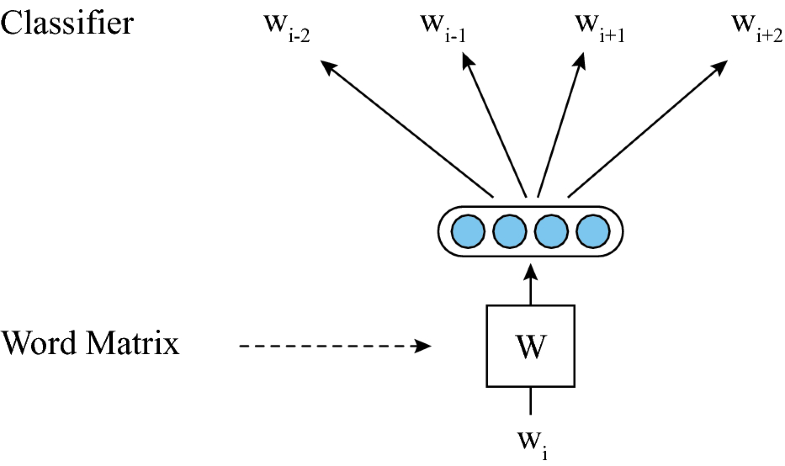
\includegraphics[width = 0.5\textwidth]{figures/skip-gram-model.png}
	\caption[The architecture of skip-gram model]
	{ The architecture of skip-gram model.}
	\label{fig:skip-gram-model}
\end{figure}

One of the widely used distributed word representation is Skip-Gram model (see Fig.~\ref{fig:skip-gram-model}) which is part of the \textbf{Word2Vec} library. It was created by a team of researchers led by Tomas Mikolov at Google. The main idea is to represent words by means of its neighbors. It tries to predict all neighboring words(the context) of a given word. According to paper~\cite{mikolov2013distributed}, the objective of model is defined as follows:$$\frac{1}{T}\sum_{t=1}^{T}\sum_{-c\le j\le c,j\ne 0} \log_{ p(w_{t+j}\mid w_t) }$$
where w is training word and c is the size of context. So its objective is to find word representations that can predict surrounding words.

Another member of distributed word representations is \textbf{Global Vectors for Word Representation(GloVe)} which is an abbreviation for Global Vectors. While Word2Vec captures certain local context window, GloVe exploits overall co-occurrence statistics of words from corpus, which is a large collection of texts. It consists of two important steps. First one constructs a matrix of term co-occurrences. For each word we compute conditional probability, e.g. for word water $ P(k\mid water) $, where $ k $ is word from vocabulary. If $ k $ is stream, the value of $ P $ is high, and if $ k $ is fashion, then expected value is low as they do not usually co-occur together. After performing all statistical computations, the large matrix is formed. Then high-dimensional context matrix is reduced by normalizing counts and log-smoothing.

\chapter{Proposed Framework}
\label{chap:framework}
In this chapter, we will introduce our proposed framework(see Figure~\ref{fig:my_model}) based on the Transformer models in detailed.But before that, we would like to explain our thoughts on the preliminary stage of the thesis, our first method: Pixel-base attention.


\section{Pixel-based attention}\label{sec:pixel_base}

We are inspired by Encoder Self-Attention in DETR, and its output attention map can intuitively distinguish each object in the image(see Figure~\ref{fig:detrattentionmap}). Therefore, we envisage using multi-self attention to intuitively distinguish the relationship between objects in the image.

\subsection{Idea of Pixel-based attention}

We input the down-sampled image features into the Multihead Self-Attention module. According to the Equation~\ref{equ:self_attention}, we will get the attention weight between each pixel in the down-sampled image feature. Assuming that in Figure~\ref{fig:ideamethod1} we obtained the down-sampled image feature size of 512x66x50 through the backbone, that is, each layer od the feature has 3300 pixels, we convert it into a sequence of 3300x512, then input it into the Multihead Self-Attention module, and get an attention map size of 3300x3300 . We look for the pixel of the subject in the row of the attention map, and look for the pixel of the object in the column of the attention map ,to find the attention weight between the subject and object pixels. Eg. the ground truth pair $ \left\langle roof, building \right \rangle $ in Figure~\ref{fig:ideamethod1} is located in the attention map as shown in the lower right corner of Figure ~\ref{fig:ideamethod1}.

\begin{figure}[H]
	\centering
	\subfigure[The attention from the first pixel of object1 to the whole image.]{
		\begin{minipage}[t]{15cm}
			\centering
			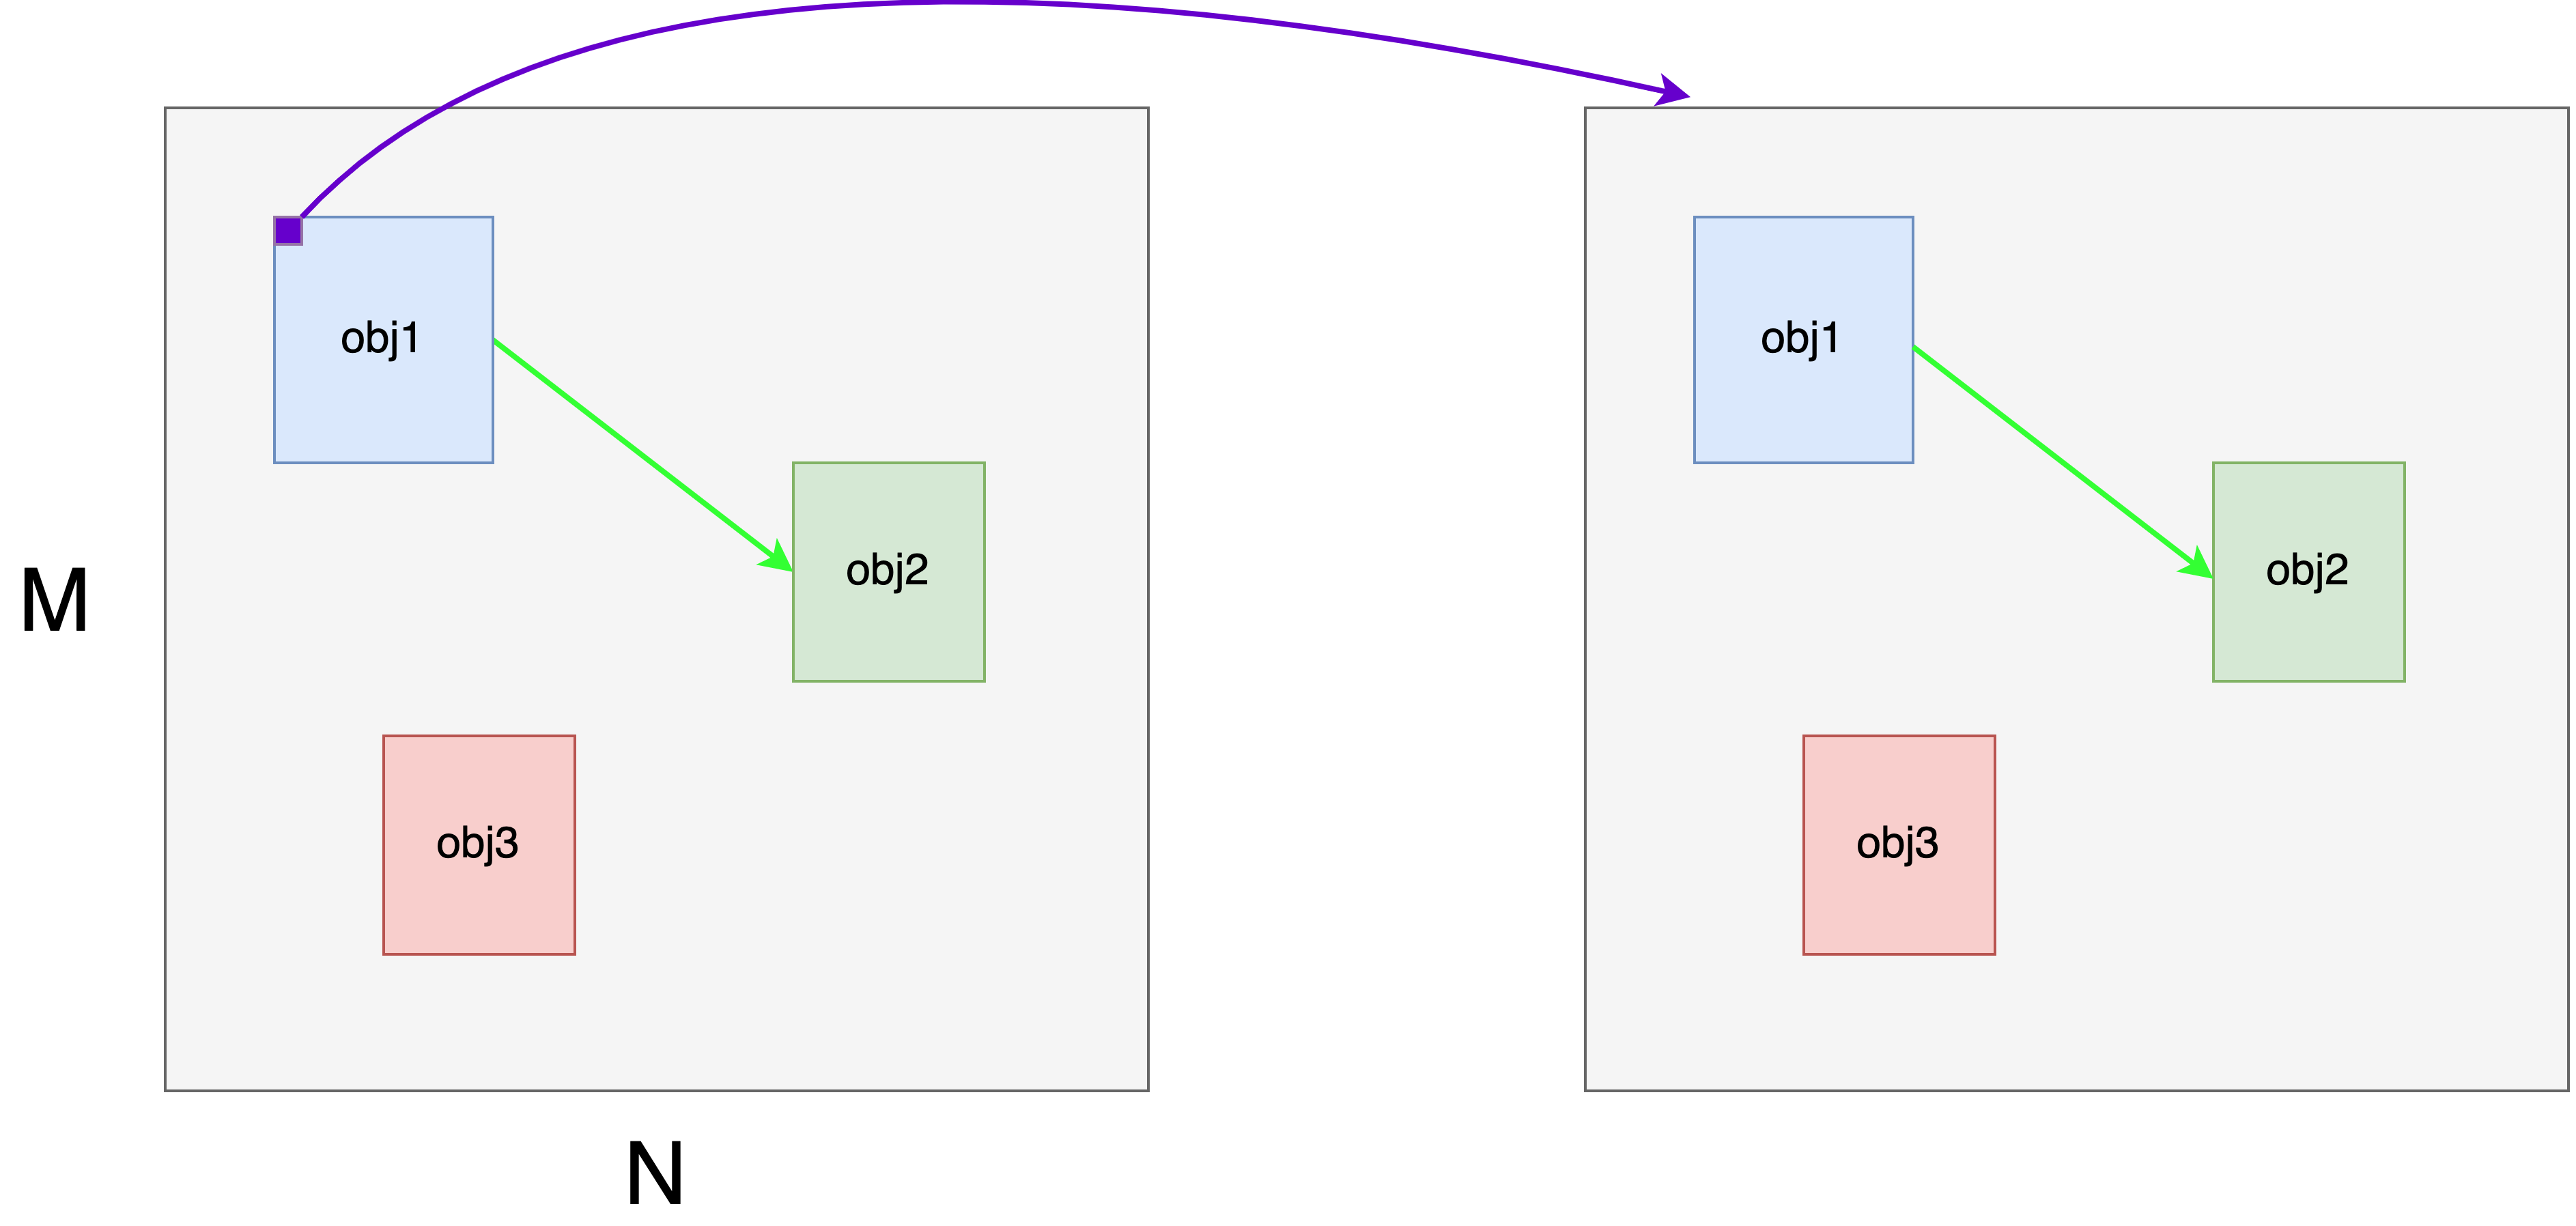
\includegraphics[width=0.8\linewidth]{figures/pixel_attention_idea}
			\label{fig:idea_pixelloss_a}
	\end{minipage}}
	
	\subfigure[The relationship between objects.]{
		\begin{minipage}[t]{7cm}
			\centering
			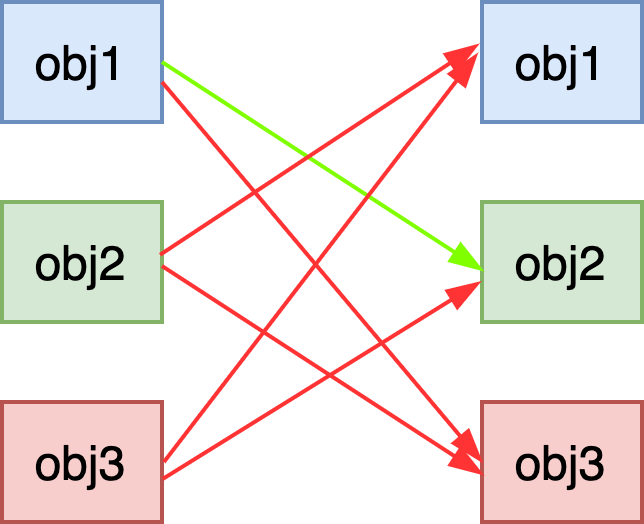
\includegraphics[width=0.8\linewidth]{figures/pixel_relation}
			\label{fig:idea_pixelloss_b}
	\end{minipage}}
	\subfigure[The attention map of each pixel of the image feature.]{
		\begin{minipage}[t]{7cm}
			\centering
			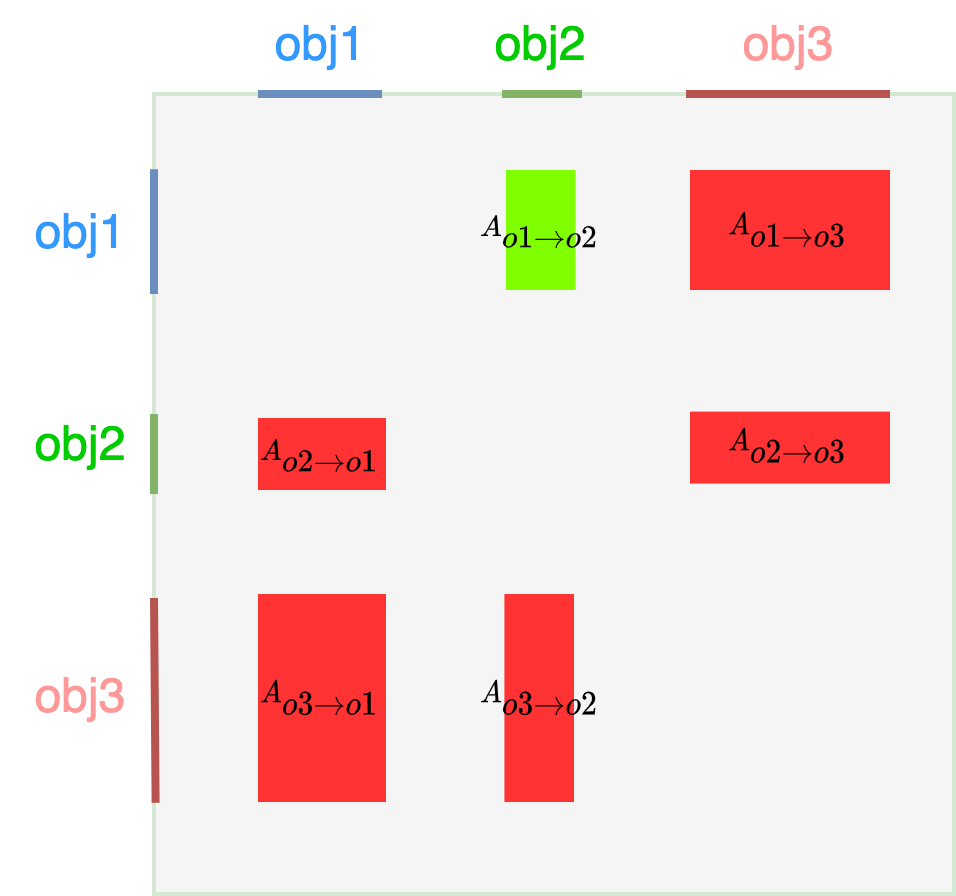
\includegraphics[width=0.9\linewidth]{figures/pixel_attentionmap}
			\label{fig:idea_pixelloss_c}
	\end{minipage}}
	\caption[The idea of the pixel attention loss]{The idea of the pixel attention. The Fig. (a) shows, that there is only relationship between $obj_1$ and $obj_2$(the green line),there are no relationship between the others. The Fig. (b) show the position of the realtion pair. The green area means realtionship, the red area means no relationship. $A_{oi \to oj}$ means the attention weights of the pixel of $obj_i$ to  the pixel of $obj_j$.}
	\label{fig:idea_pixelloss}
\end{figure}

We hope that through the training of our model, the attention weight of ground truth pairs can be higher than those of pairs without relation. In this way, we can use the attention weight in the evaluation to determine which pairs are most likely to be related.
\begin{figure}[!htbp]
		\centering
	\subfigure[No relation between \textit{roof} and \textit{tree}.]{
		\begin{minipage}[t]{6cm}
			\centering
			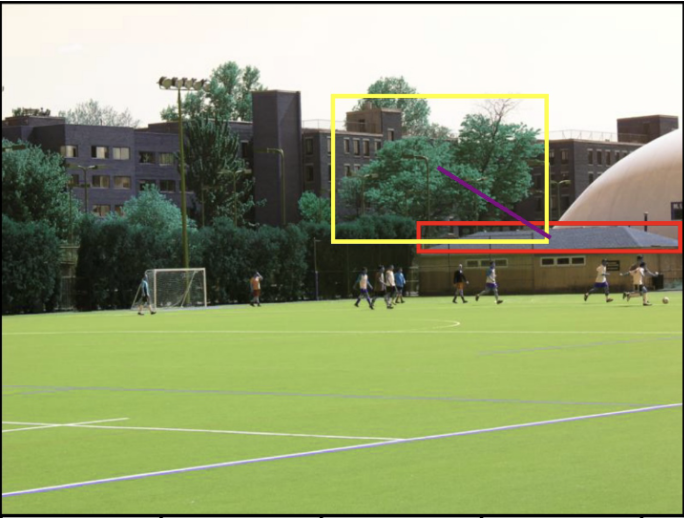
\includegraphics[width=1\linewidth]{figures/roof/img1}
	\end{minipage}}
	\subfigure[The attention of $<roof, tree>$.]{
		\begin{minipage}[t]{6cm}
			\centering
			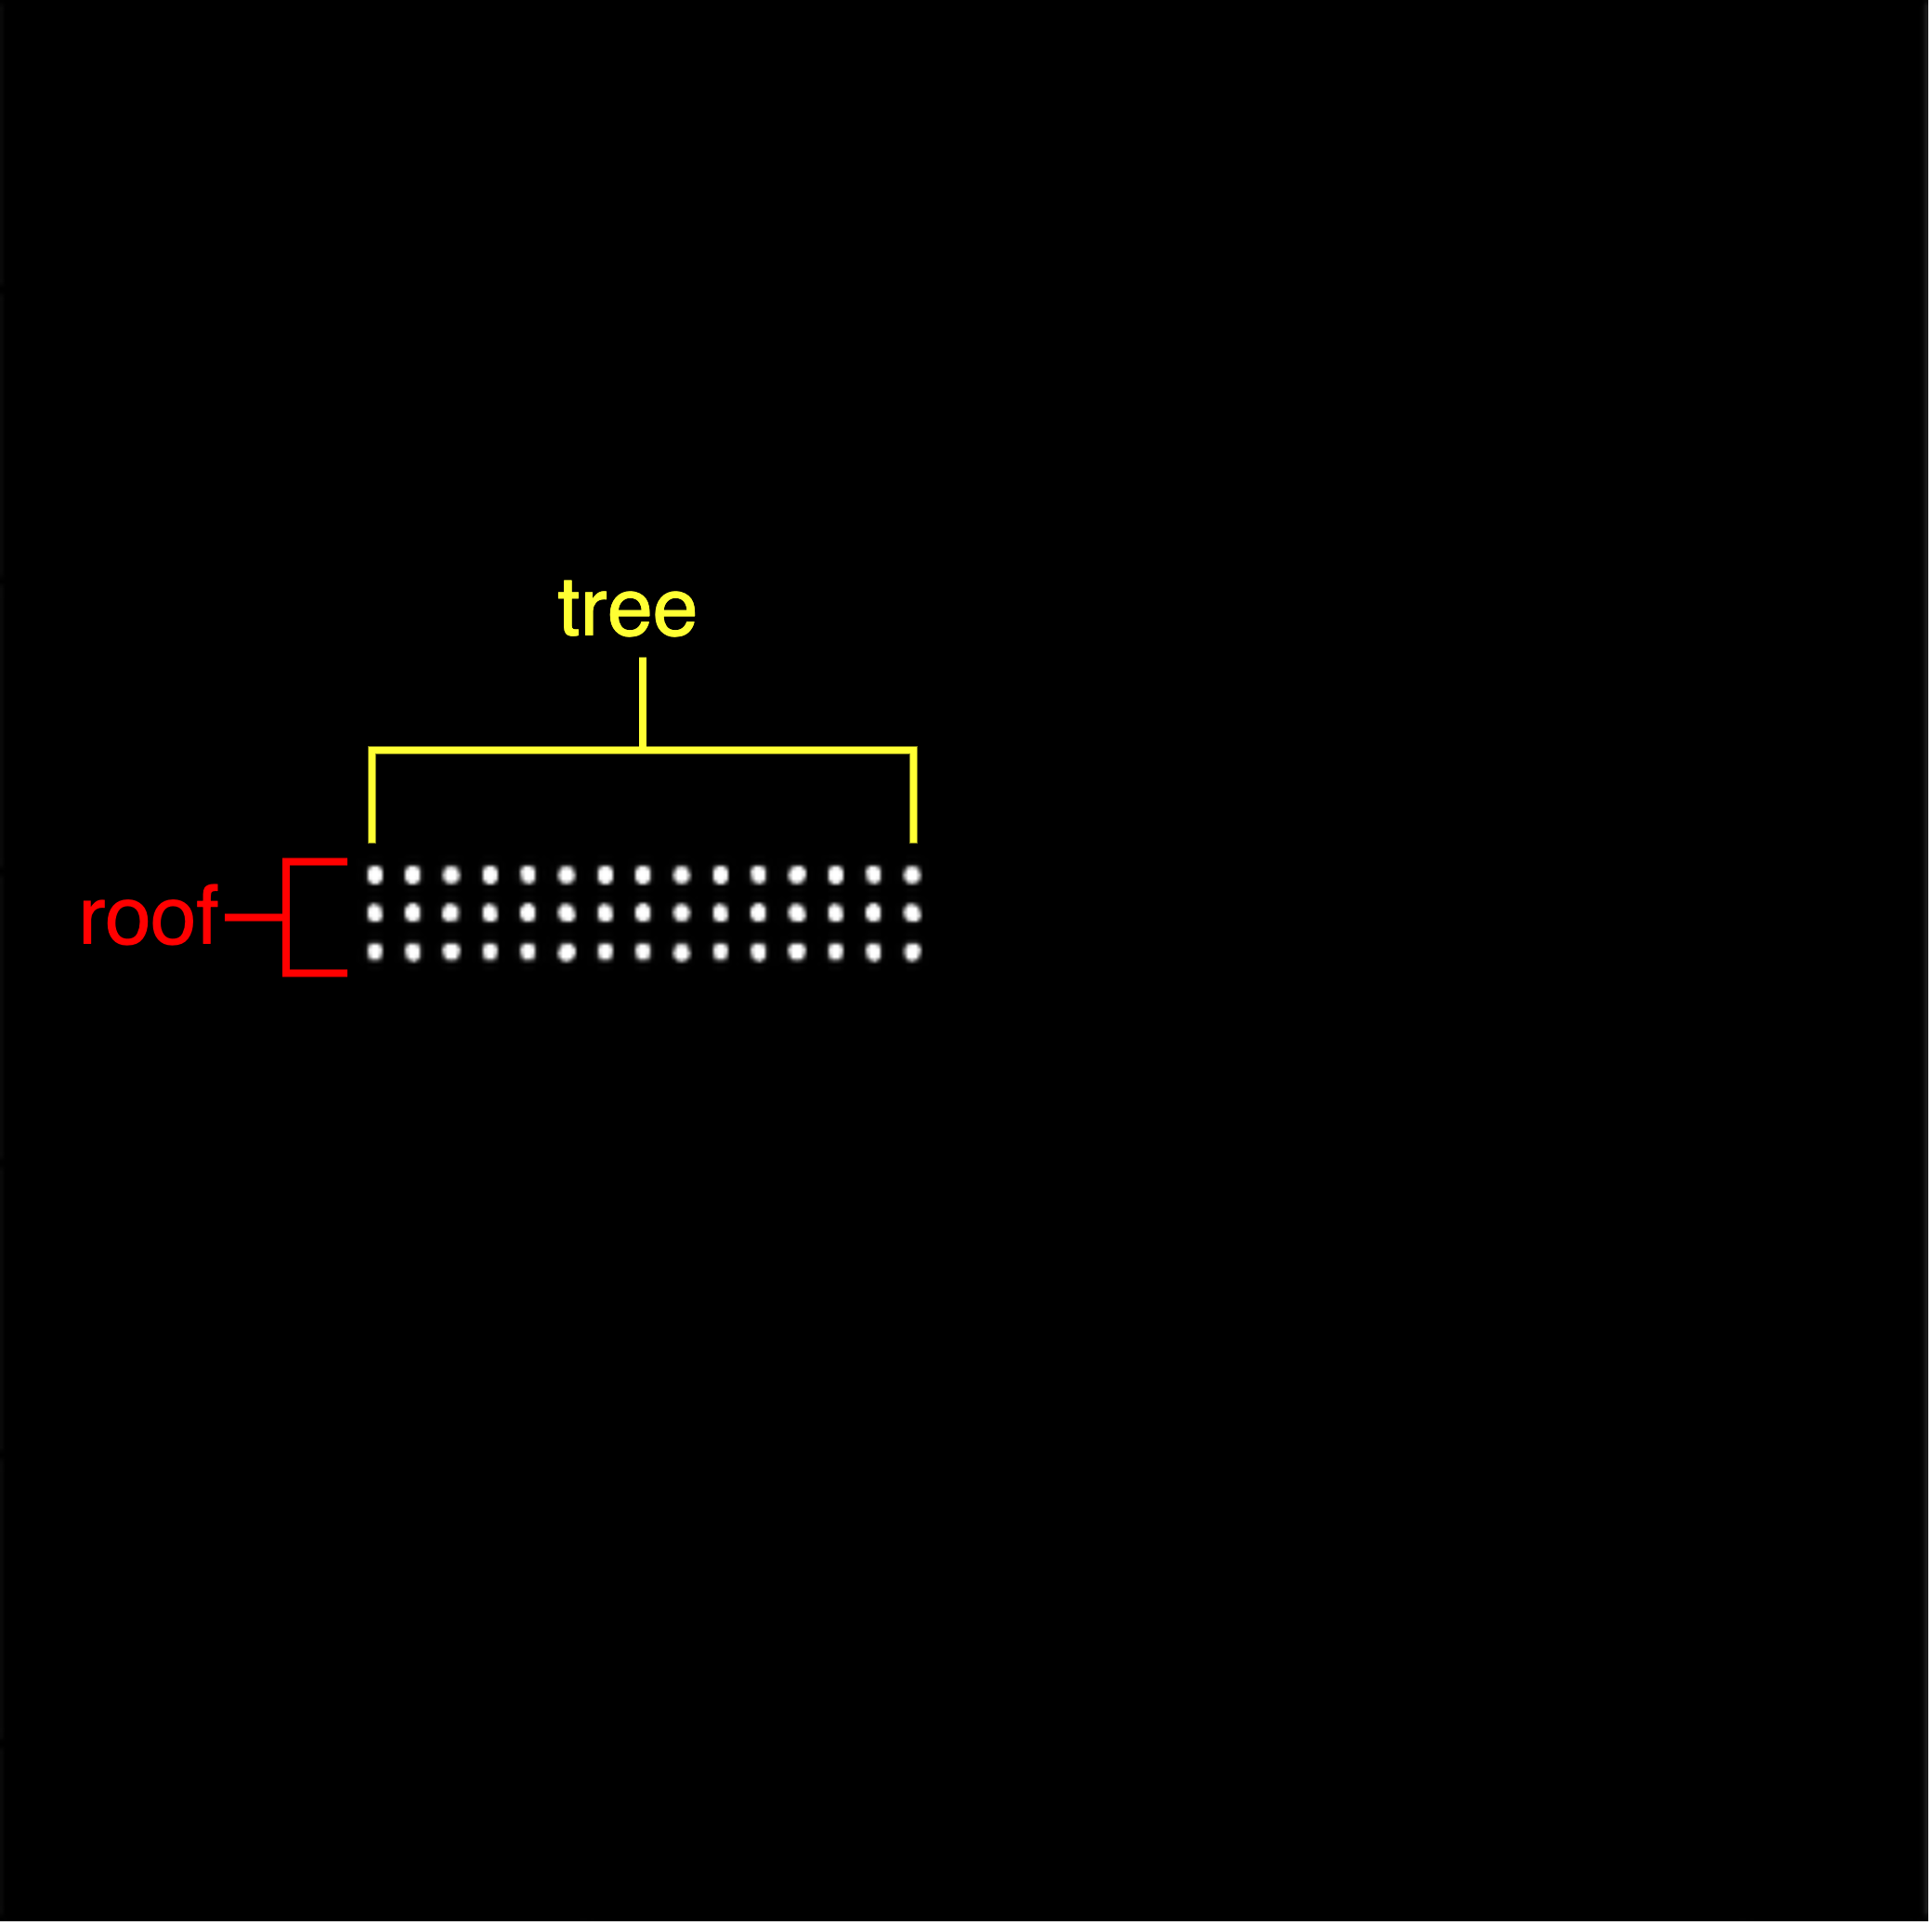
\includegraphics[width=0.8\linewidth]{figures/roof/map1}
	\end{minipage}}
	
	\subfigure[GT relation: \textit{roof on building}.]{
		\begin{minipage}[t]{6cm}
			\centering
			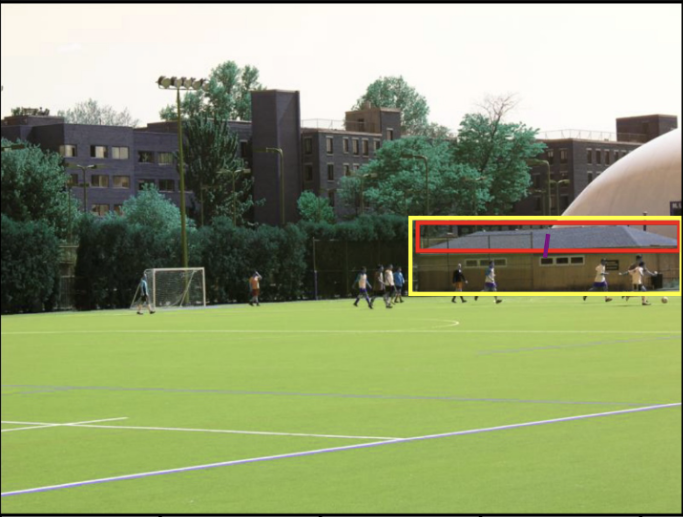
\includegraphics[width=1\linewidth]{figures/roof/img2}
	\end{minipage}}
	\subfigure[The attention of $<roof,building>$]{
		\begin{minipage}[t]{6cm}
			\centering
			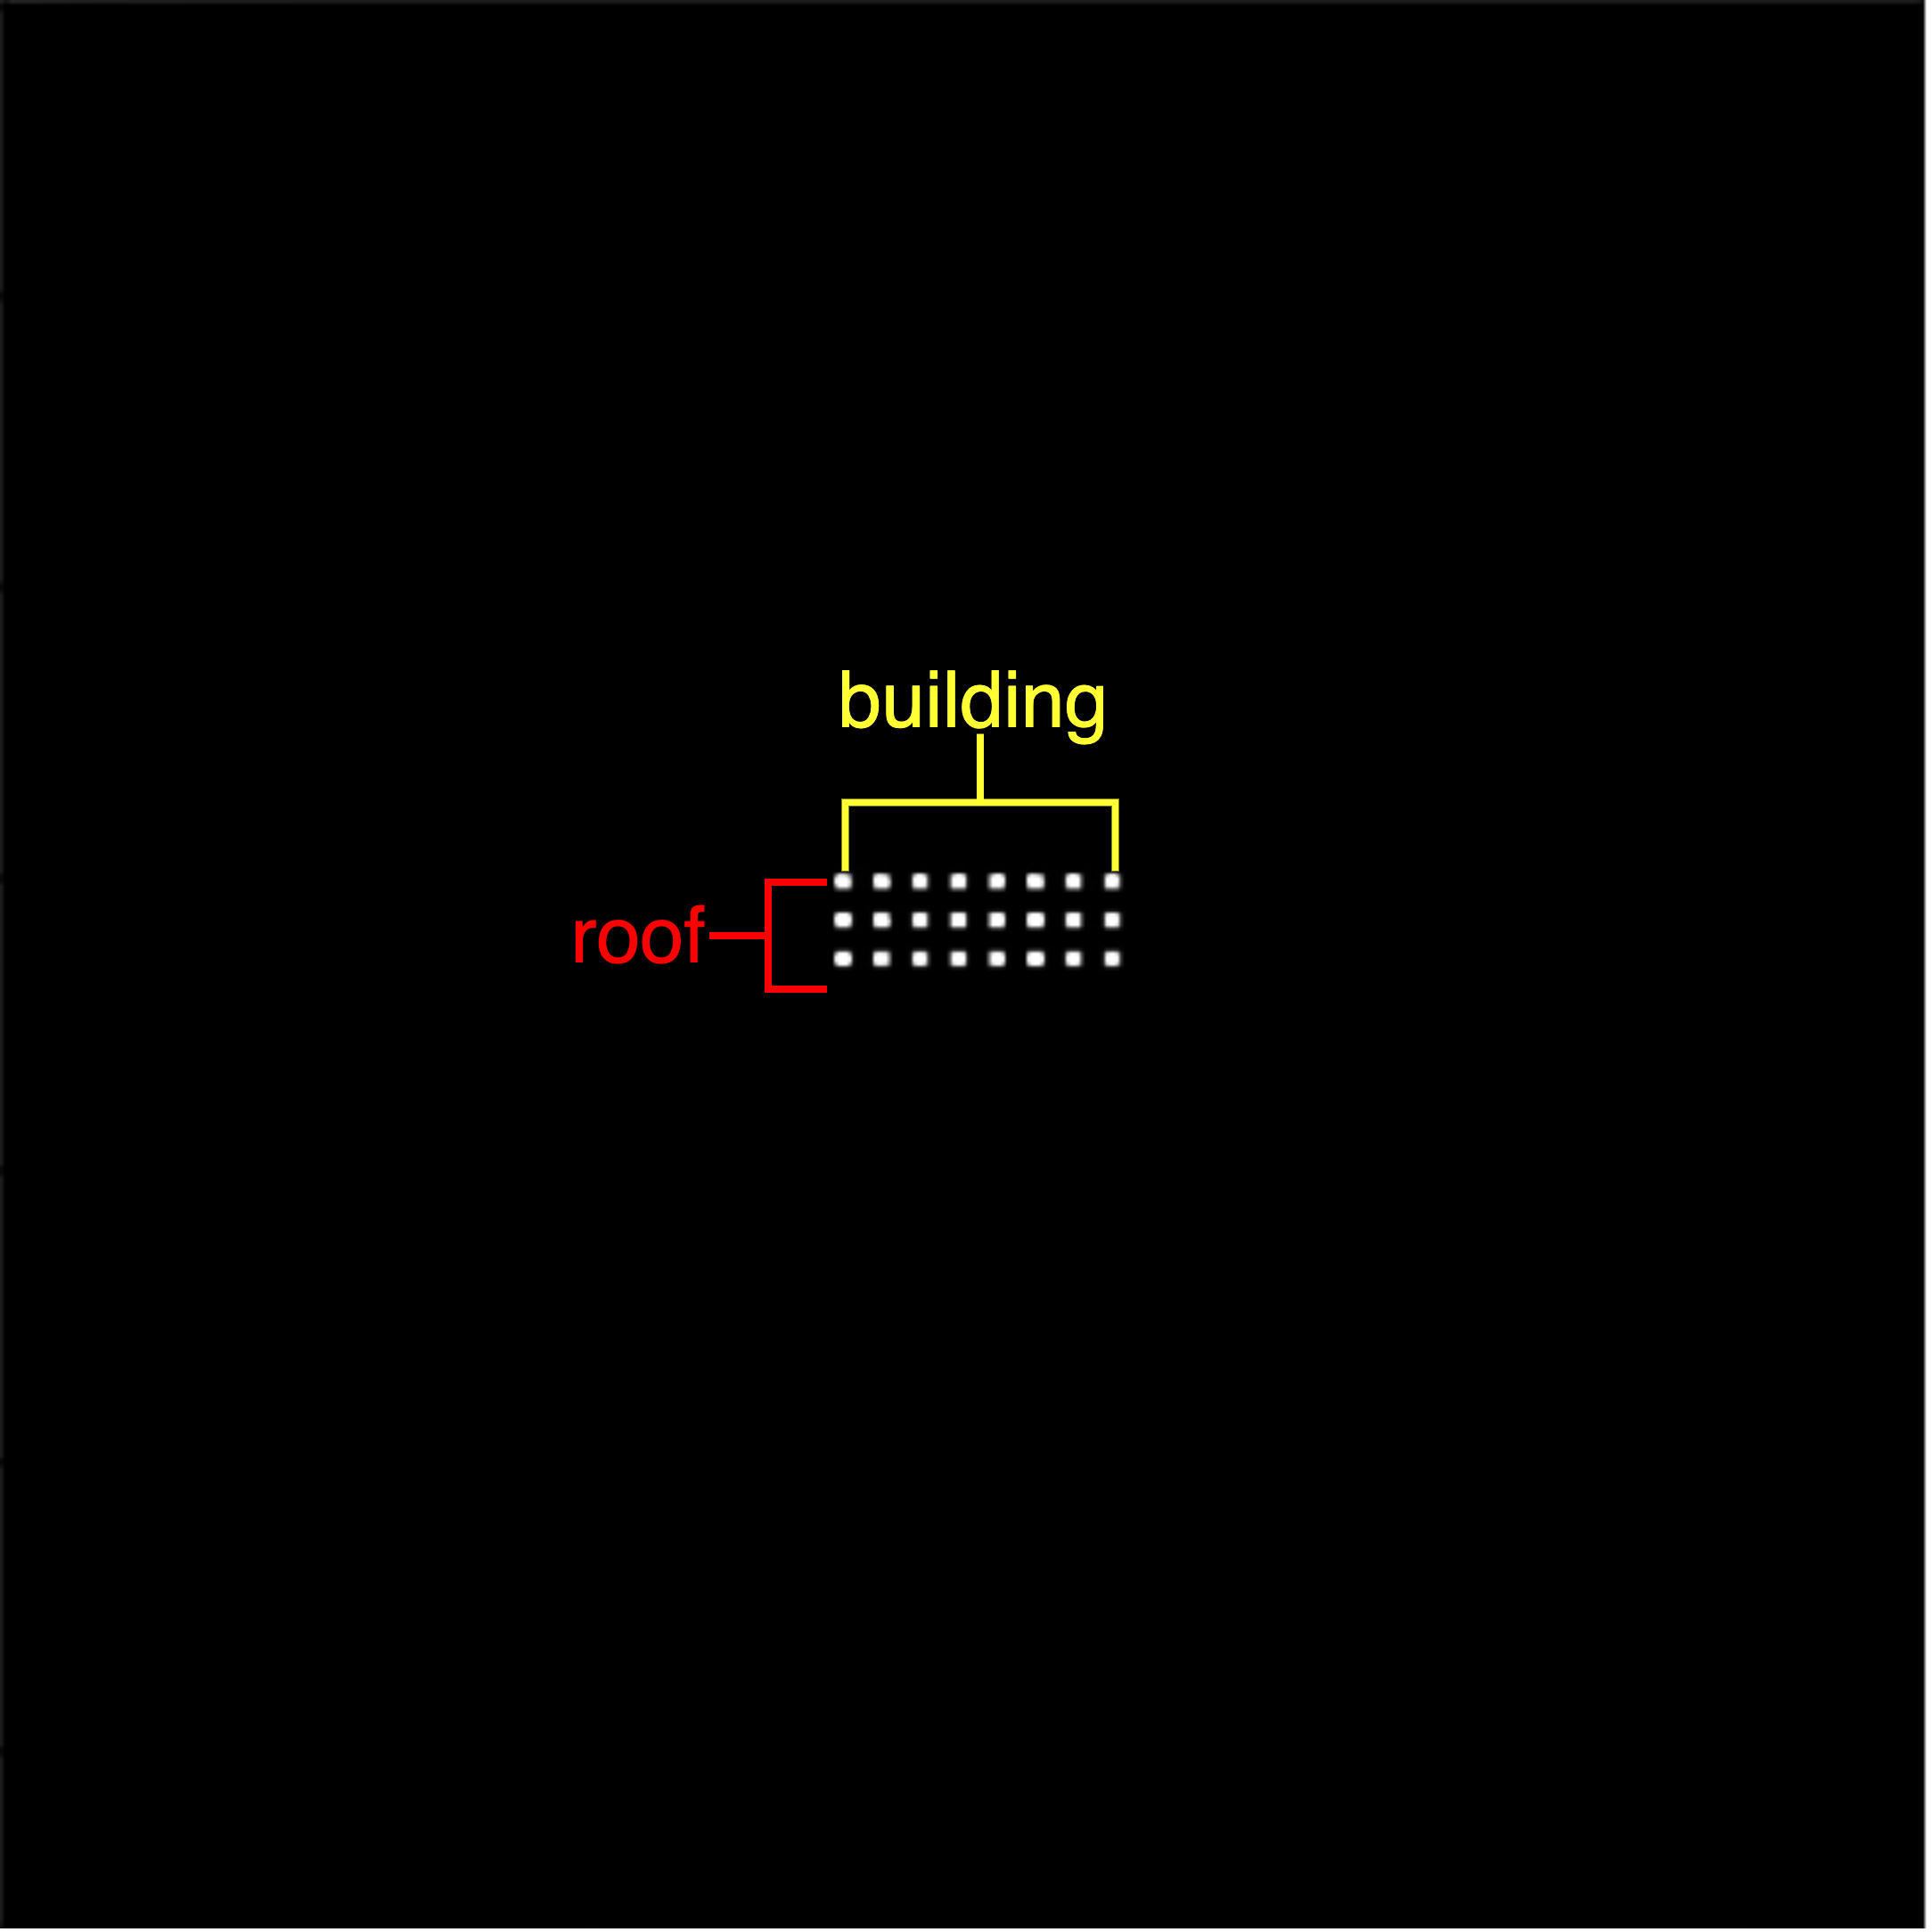
\includegraphics[width=0.8\linewidth]{figures/roof/map2}
	\end{minipage}}

	\caption[An example of Pixel-based attention]{Relation pair on image and its position on attention map.}
	\label{fig:ideamethod1}
\end{figure}

\subsection{ Prototype model}
The concrete realization of our idea is as follows: As shown in following Figure~\ref{fig:method1baseline}, first we input an image into the  backbone VGG16~\cite{simonyan2015deep}(see Figure~\ref{fig:vgg16}.) to gets a down-sampled image feature \textit{feature} ,  then it passes through a Multi-Head Self-Attention module to get an attention map and new image feature \textit{feature2}. Finally, the feature of the subject-predicate object is extracted by ROI Align(see in Section~\ref{fig:roialign}), and sent to the predicate classifier as input.


\begin{figure}[H]
	\centering
	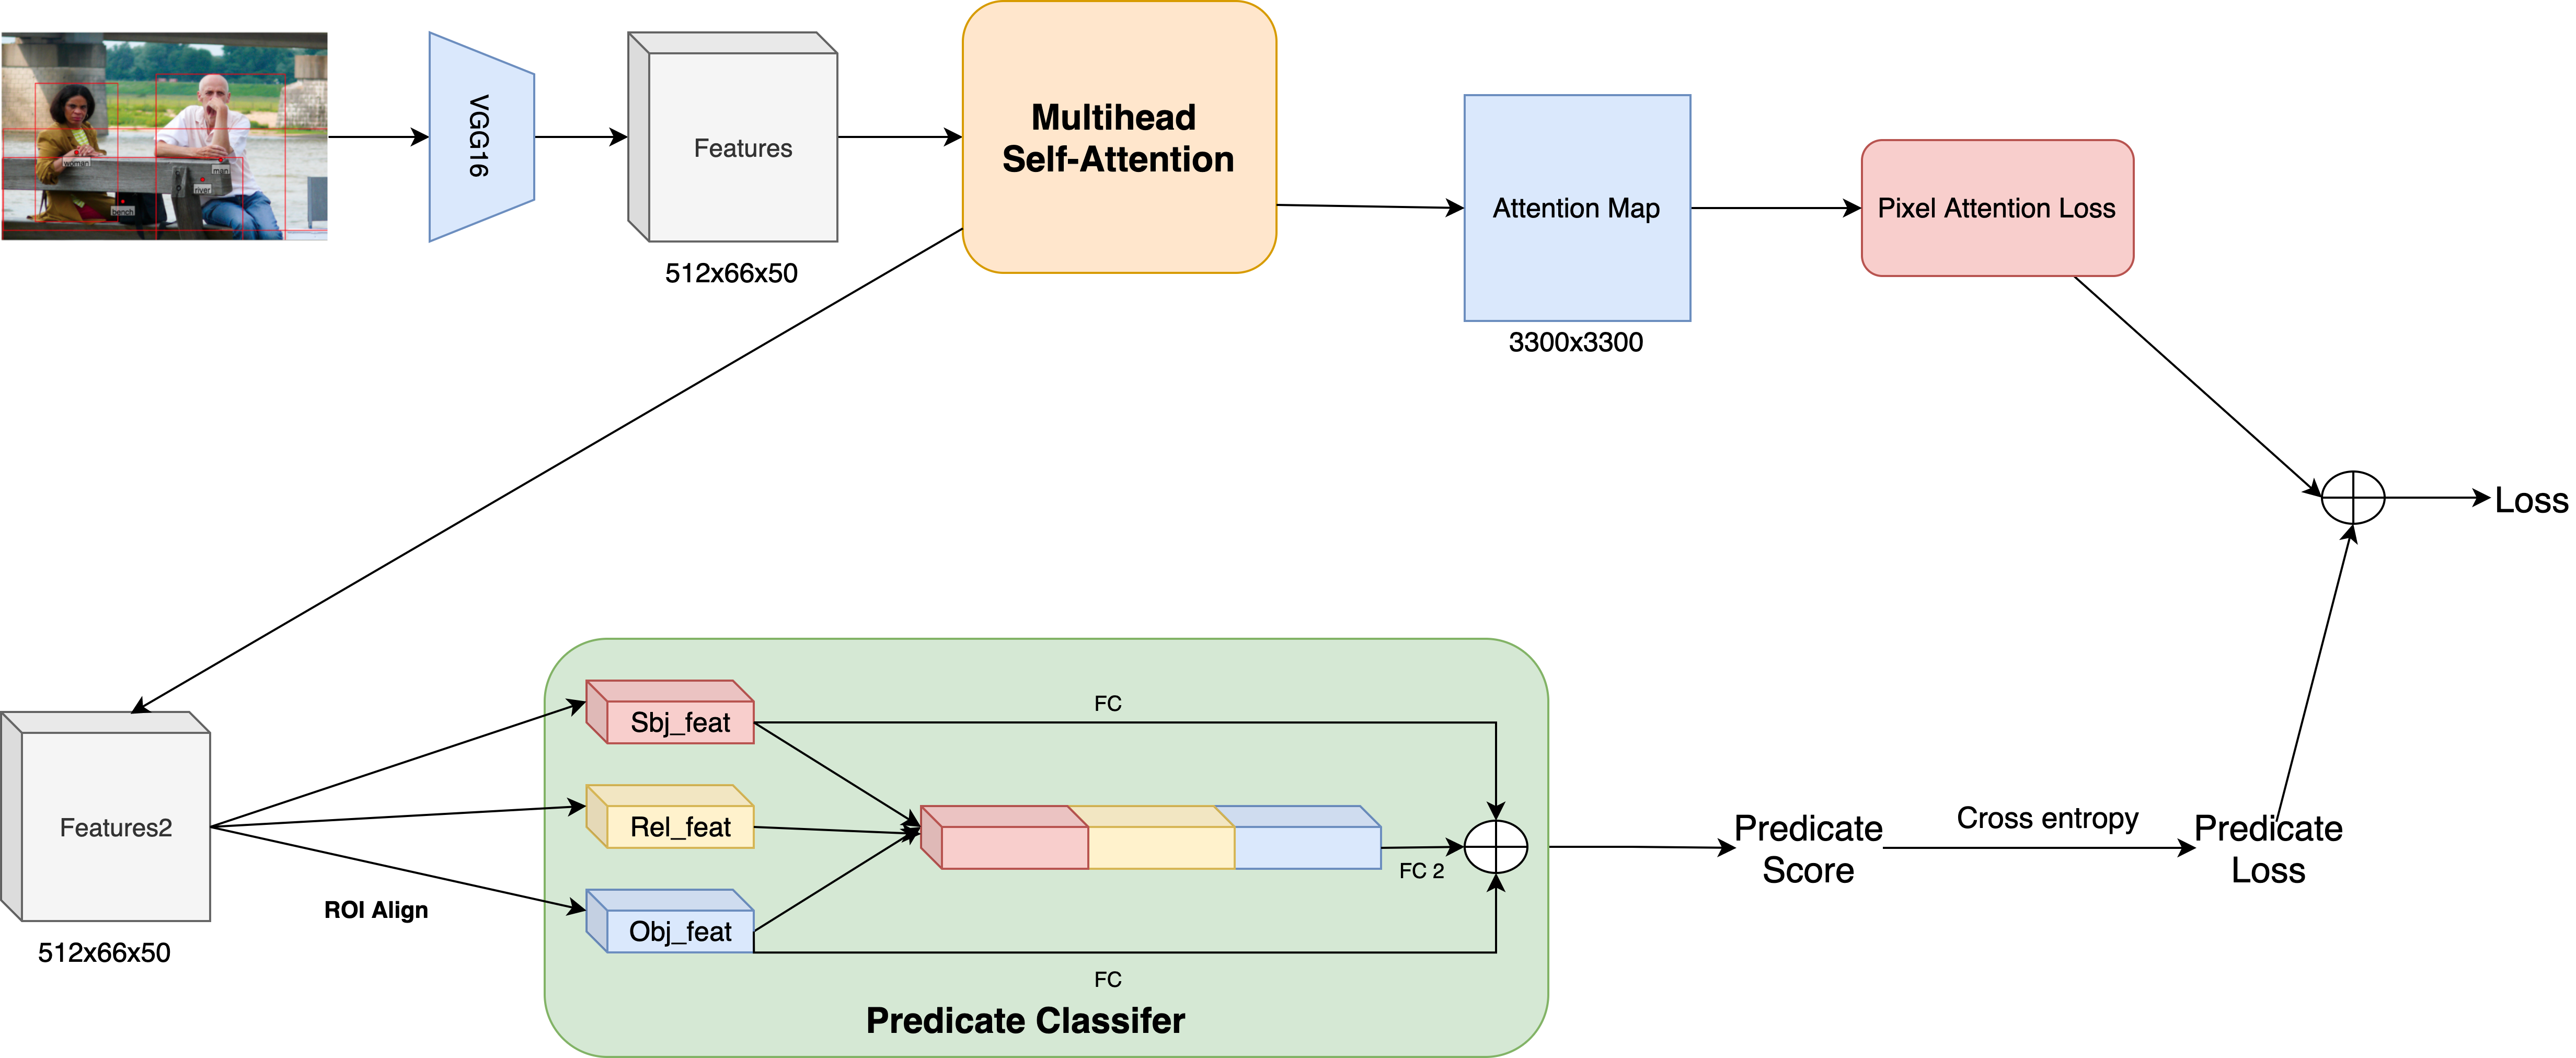
\includegraphics[width=1\linewidth]{figures/method1_baseline}
	\caption[The baseline of the first method: Pixel-based attention]{The baseline of the  first method: Pixel-based attention}
	\label{fig:method1baseline}
\end{figure}

\subsection{Pixel  Attention Loss}

We have studied the attention map, and its meaning is the attention between all pixels of the image feature( $ Attention_{p_i\to p_j}, \  wehre \quad p_i,p_j\in \mathbb{P}_{img} $) , $ \mathbb{P}_{img}  $is a collection containing all pixels of the image feature from VGG16.

We want to know whether $ obj_i  $has a relationship with $ obj_j$ through attention. For example, we have three objects ($ obj_1 $, $ obj_2 $, $ obj_3 $) . Assuming there is a relationship between $ obj_1 $ and $ obj_2 $, $ obj_1 $ and $ obj_3 $, $ obj_2 $ and $ obj_3 $ are not related, see in Fig.~\ref{fig:idea_pixelloss_a}, the green line means $ pair <obj_1,obj_2> $ has relationship, while the red line means the other pairs have no relationship. 

We first have the following definition: 
$$ Attention_{p_{obj_i}\to p_{obj_j}},\ where \quad p_{obj_i} \in \mathbb{P}_{obj_i},\  p_{obj_j} \in \mathbb{P}_{obj_j} $$
Where $ \mathbb{P}_{obj_i}, $ represents the collection of all pixels of $ obj_i $ on the image feature obtained from VGG16. $  Attention_{p_{obj_i}\to p_{obj_j}} $ means the attention weight between the pixel $ p_{obj_i} $ and the pixel $ p_{obj_j} $. In Fig.~\ref{fig:idea_pixelloss_b} we abbreviate it as $ A_{oi \to oj} $. and we can see the green area means there is a relationship.



we want to know which pair is more relevant in evaluation through the attention weights between each pixel on the down-sampled image feature, thus we design a pixel attention loss as following:
\begin{equation}\label{pixel_attention_loss}
	loss_{attention}=max(0, \frac{1}{m}\sum_{m}Att_j^{no\_rel}-\frac{1}{n}\sum_{n}Att_i^{rel}+0.25
	/3300)
\end{equation}

Where:

\begin{itemize}
	\item $ Att_j^{no\_rel} $ : the attention weight of the pixel j of no-relation pairs.
	\item $ Att_i^{rel} $ :  the attention weight of the pixel i of gt relation pairs.
	\item Margin=0.25/3300 is quarter the average of the attention map.
\end{itemize}

For example, in Fig.~\ref{fig:idea_pixelloss_b} , our $Att_i^{rel} $  is $ A_{o1 \to o_2} $ (the green area) and  the $ Att_j^{no\_rel} $ are $ A_{o1 \to o_3}  $,  $ A_{o2 \to o_1}  $, $ A_{o2 \to o_3}  $, $ A_{o3 \to o_1}  $ and $ A_{o3\to o_2}  $(the red areas). We use our attention loss to make attention weights of the green area in this figure higher and the value of the red area lower. In this way, we can judge which can have a relationship through the attention value of each pair during evaluation.

For this method, we have conducted many attempts and experiments. Through our experimental verification, we found that the results did not achieve our expectations. After thinking, we found a very serious problem. For the specific experimental results and analysis, please refer to the following chapters. So we changed our thinking, changed from pixel-based to box-based, and used the complete transformer encoder decoder structure, and added our own design here. Next we will introduce our final model Retina Net.

\section{Retina Net}
\label{sec:retinanet}
After previous trial and error, we changed our thinking and proposed our new model structure Retina-Net.we completed the three tasks of the VRD problem: \textit{predicate classification} , \textit{scene graph classification} and \textit{scene graph detection} . For these three tasks, our model is unified, based on the transformer model, and other parts such as the decoder for the relationship have been added.

In our Framework (see Fig.~\ref{fig:my_model}), we propose a new visual relationship detection network, our network consists of a convolutional neural network (CNN) backbone, an \textit{Encoder} module, \textit{Object Decoder} module to obtain object features and  the context between each entity, \textit{Relation Decoder} module to obtain the context beween entities and relation  , and a \textit{Predicate Classifer} module to predict predicate.

\begin{figure}[!htbp]
	\centering
	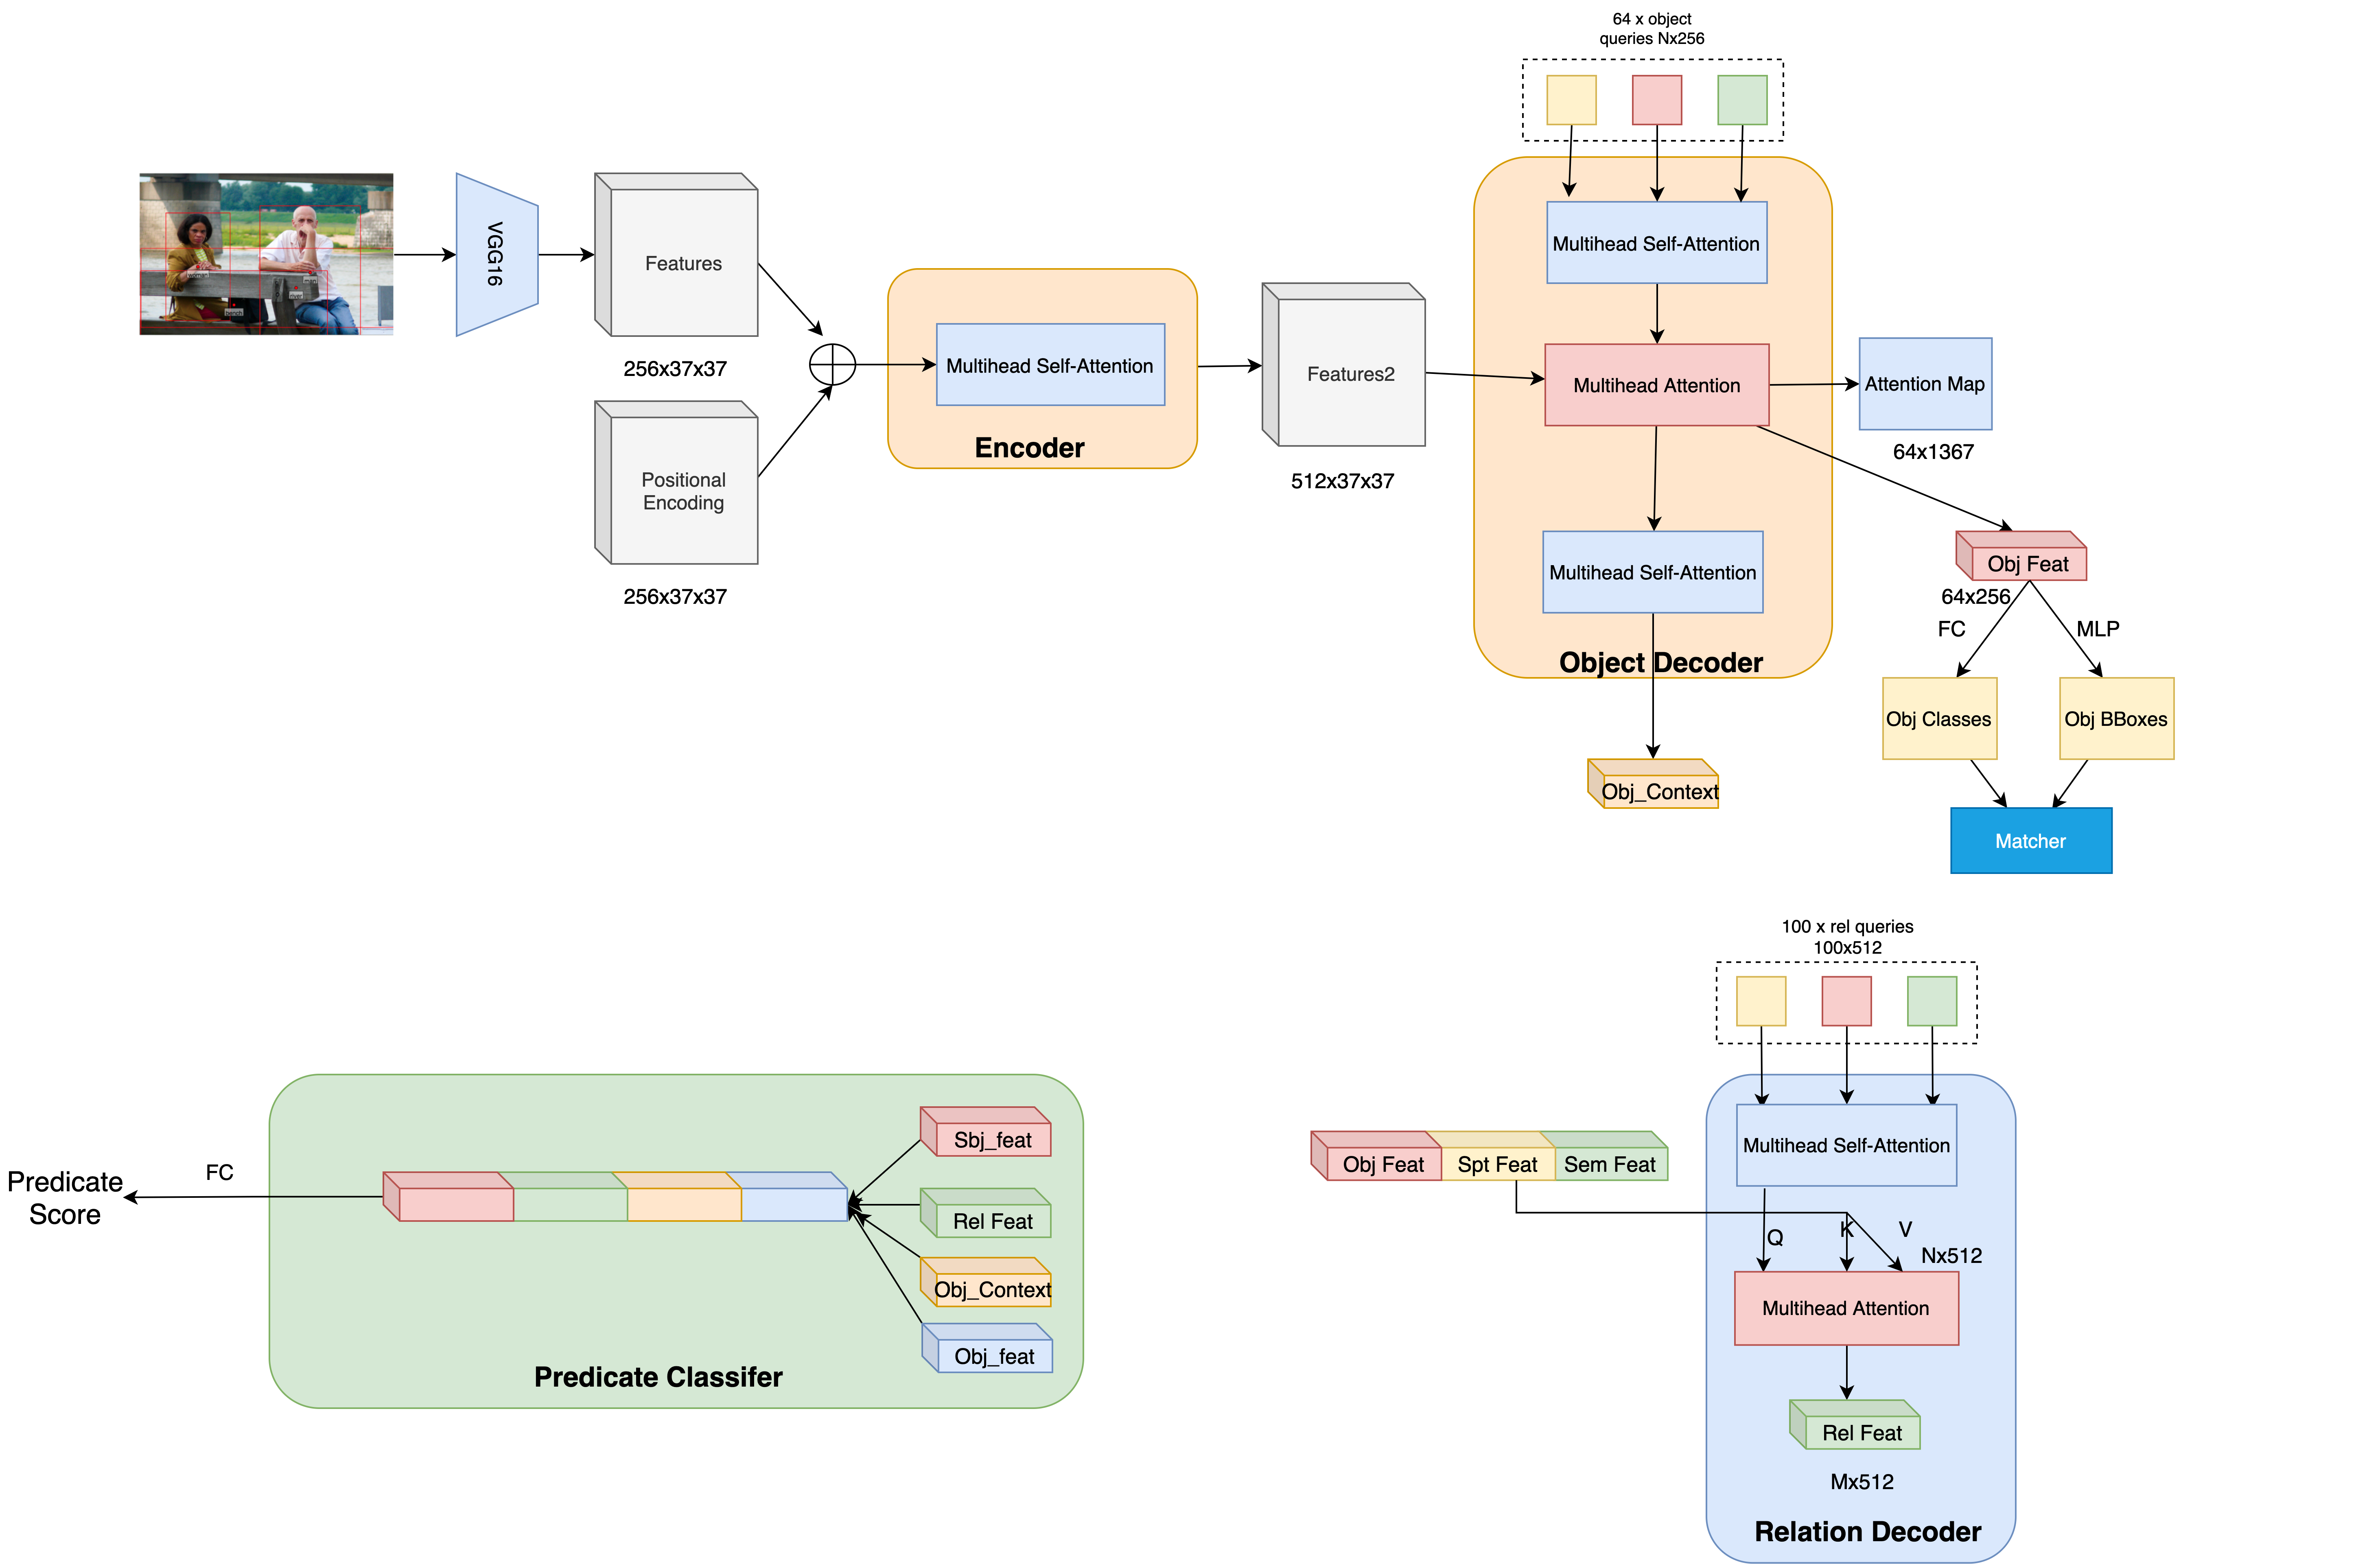
\includegraphics[width = 1\textwidth]{figures/my_model.png}
	\caption[The architecture of our model.]
	{The architecture of our model,it consists of a convolutional neural network (CNN) backbone, an Encoder, an Object Decoder, a Relation Decoder and a Predicate Classifier.}
	\label{fig:my_model}
\end{figure}


\subsection{Generation of Image Feature Maps }

We first use vgg16 to extract preliminary image features, and then generate a final image feature through an Encoder(see in Fig.~\ref{fig:imgfeatbaseline}).

In the proposed framework the VGG16 as backbone is used to extract preliminary feature maps $f^{vgg}_{img}$ and  then generate final image features $f^{en}_{img}$ through an Encoder. Before an image is fed into the VGG16 net it is rescaled and zero padded to a Tensor with the size $ 3\times592\times592 $. Then the scaled image is normalized with $ mean = [0.485, 0.456, 0.406 ]$ and $ std = [ 0.229, 0.224, 0.225]$.   The size of feature $f^{vgg}_{img}$ is $512 \times 37 \times 37$. Before we input it into the encoder, we need to convert $f^{vgg}_{img}$  into a sequence tensor.In order to reduce the parameter size, we set the size of the sequence element to 256, that is, the number of feature layers is changed from the original 512 to 256, so we need to add a convolutional layer between vgg16 and the encoder, whose stride and kernel size are both 1. Finally we will set the size to $ 1369 \times bs \times 256 $, where $ 1369 $ is the sum of down-sampled pixels of each layer in image feature $f^{vgg}_{img}$ ($ 37 \times 37 = 1369$), $ bs $ is our batch size, and $ 256  $is the size of the feature of each sequence. The size of the output feature $f^{en}_{img}$ is same as that of the input ($ 1369 \times bs \times 256 $), we can also reshape the output to the size of $256 \times 37 \times 37$.


\begin{figure}[tbph!]
	\centering
	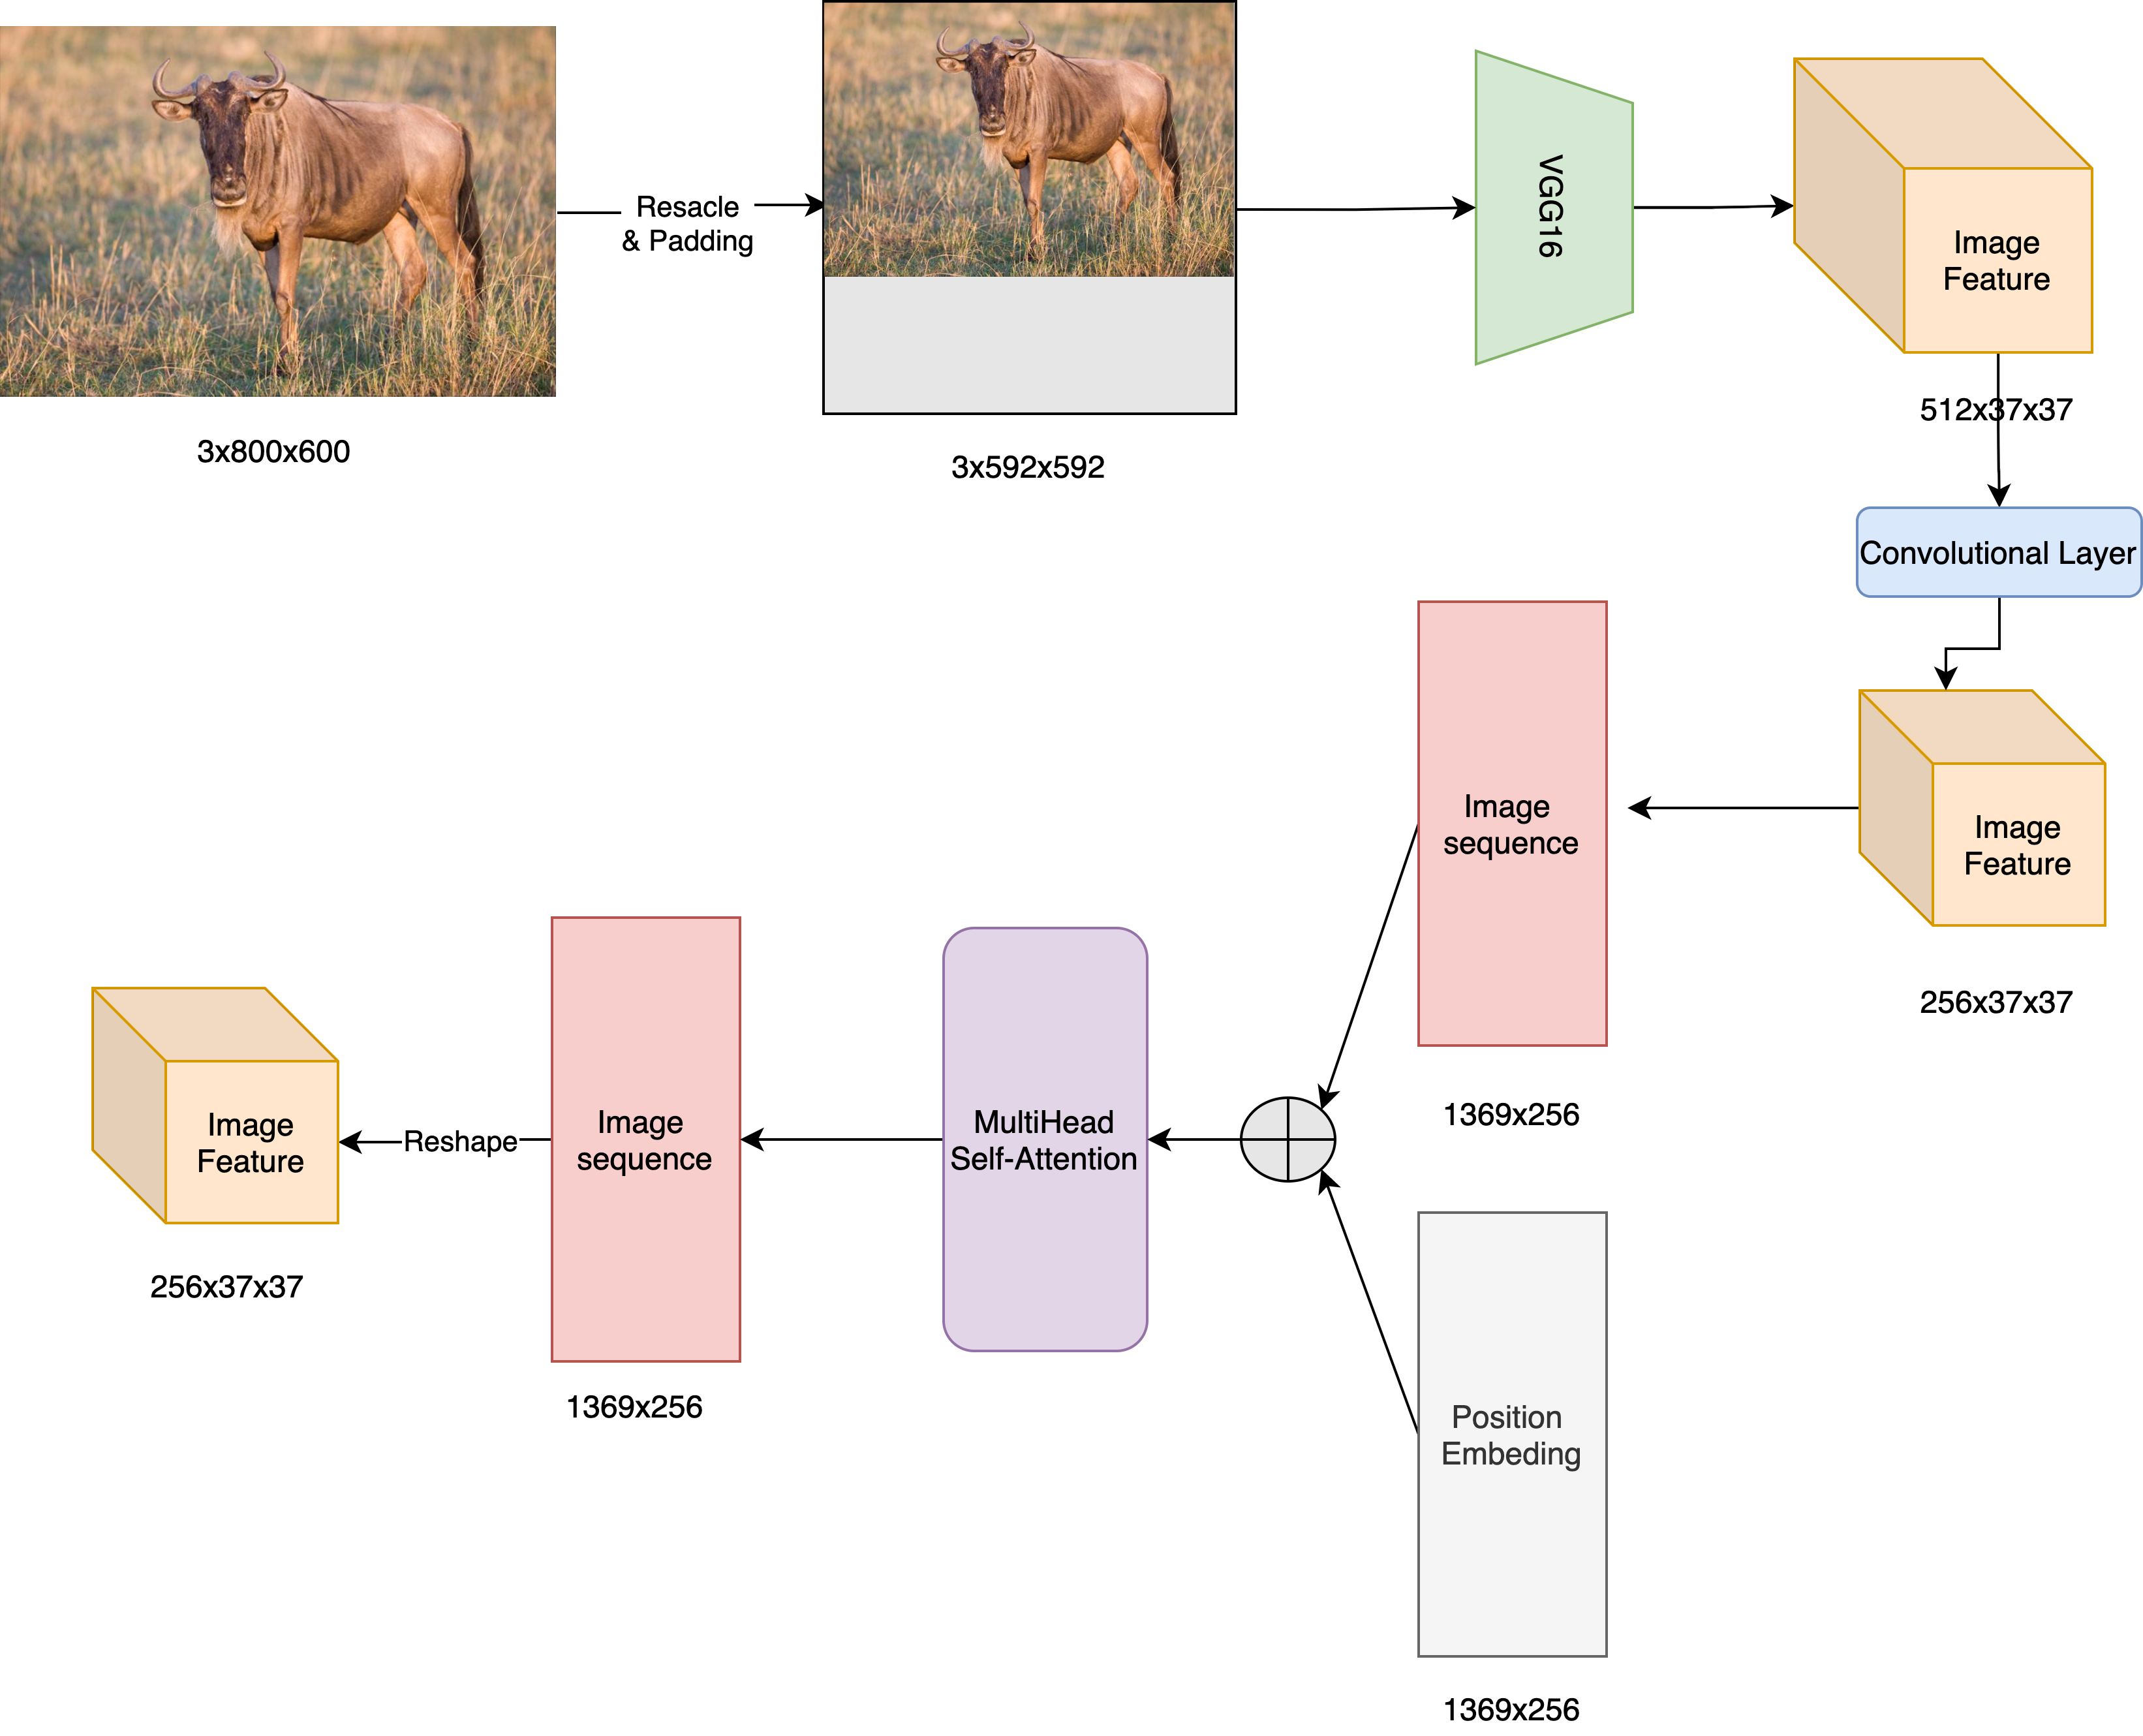
\includegraphics[width=0.9\linewidth]{figures/img_feat_baseline}
	\caption[Generation of Image Feature Map]{Illustration of the generation of image feture map.}
	\label{fig:imgfeatbaseline}
\end{figure}


Ours Encoder is a MultiHead Self-Attention module, whose input is an image sequence tensor plus a  Position Embedding tensor. Different from the processing of sequence signals by the RNN network, the Self-Attention module processes the sequence in parallel, so it does not know the order of the sequence, we need to add position information to the original sequence.  we are processing two-dimensional image information, thus we need to add two-dimensional position information for each pixel. We use Equ.~\ref{equ:position_embedding} to encode the position of the picture pixels.


\subsection{Object Decoder }

In this part we will introduce a very important part of the model: \textit{Object Decoder}. We use a custom object query to obtain the object feature and context between each entity through three Multihead Attention models(see Fig.~\ref{fig:objectdecoder}).

\begin{figure}[tbph!]
	\centering
	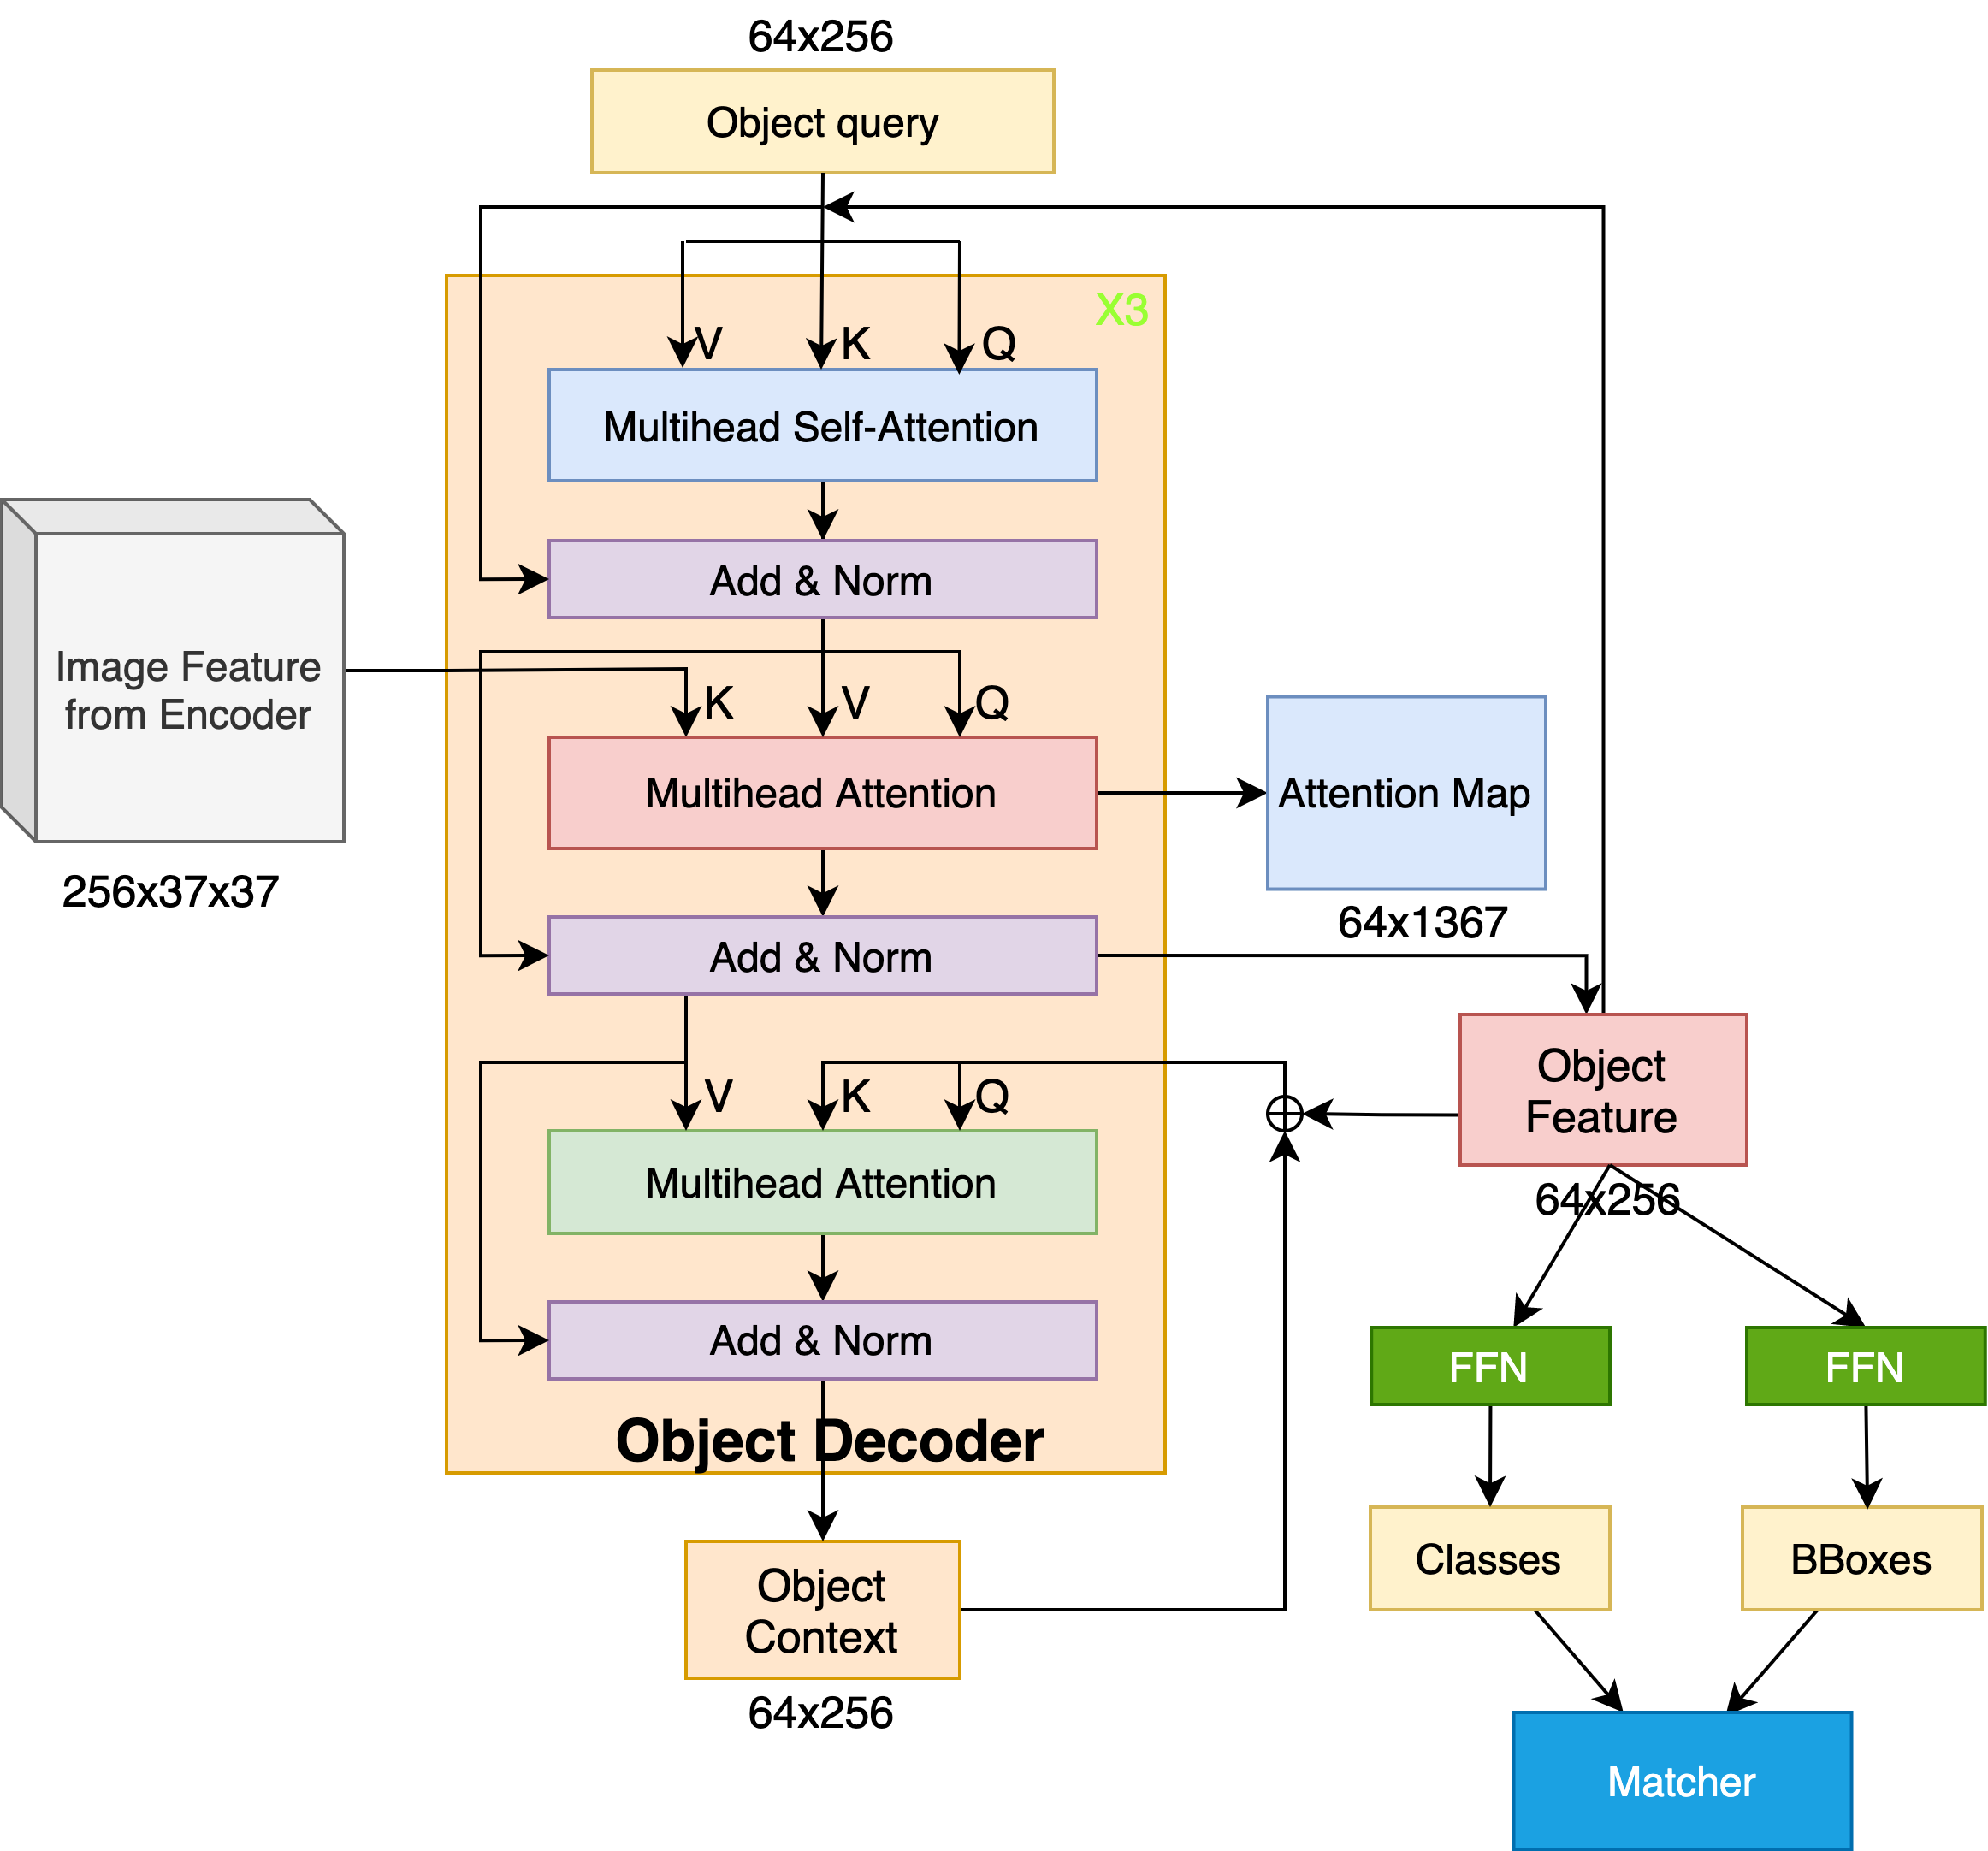
\includegraphics[width=0.9\linewidth]{figures/object_decoder}
	\caption[Illustration of the Object Decoder]{The architecture of the Object Decoder, it consists of three Multihead Attention modules,it can obtain three outputs, Attention Map, Object Feature and Object Context.}
	\label{fig:objectdecoder}
\end{figure}

%\subsubsection{The overview of Object Decoder}
As shown in Figure~\ref{fig:objectdecoder}, our decoder structure is similar to the decoder structure in the traditional transformer~\cite{vaswani2017attention}. The difference is that we added a new Multihead Attention  (see the light green part in  Figure~\ref{fig:objectdecoder}). module after the second MultiHead Attention module. In addition, we adopted the Multihead Attention of 8 heads 3 layers. We have also made changes to the object query, which we will explain in detail in the following part.

%We obtained the object feature and an attention weight map in the second Multihead Attention module (see the red part in the middle of Figure~\ref{fig:objectdecoder}). Obtain the object context through the third Multihead Attention module. This means the context of one entity to other entities. For example, we have 10 object entities in a picture. The attention map generated by the second Attention module is the effective part of $ 10 \times 10 $. Of course, the size of the attention map should be $  64\times 64 $ showed in Fig.~\ref{fig:objectdecoder}, but we only have 10 valid entities and the other 54 will be filled with 0 .So the attention map will have an effective part of $ 10 \times 10 $. Its meaning is the attention weight of an entity to other entities, including itself, that is, we have obtained a global context.It is worth mentioning that in the first layer of the Object Decoder operation, we initialize the object context to all zero tensor.


%%We can simply derive each output through Equ.~\ref{equ:self_attention}. We set the image feature from encoder be $f_{img}$, the Object Feature is $ f_{obj} $ ,the object context is $ C_{obj} $, and the attention map from the seconde Attention module is$  Att $.




\subsubsection{Object query}
In related papers (such as DETR~\cite{carion2020end} and Deformable DETR~\cite{zhu2021deformable}), using transformers for object detection, in addition to only one picture information, it is necessary to make predictions of classes and bounding boxes, so they use the learnable obeject query: they used the weight of an embedding layer as the object query. First of all, the interpretability of this query is very poor and has no actual physical meaning. Moreover, in the three tasks of VRD: SGCLS provides the entity's bounding box information, and even the PREDCLS task provides category information. Therefore, in these two tasks, we can make full use of the known information and propose a new entity encoding method to use as an object query.Since the known conditions provided by the three tasks of VRD are not the same, we use different queries.


In this thesis, we propose a custom object query for PREDCLS and SGCLS tasks, as shown in Fig.~\ref{fig:objectquery}. In these two tasks, the bounding box is known information, so we first project the box information of the form $ (x1y1x2y2)  $(where$ [x1,y1] $ is the coordinate of the upper left corner of the box, and $ [x2,y2] $ is the coordinate of the lower right corner of the box)on a size of $ 37 \times 37 $ mask. We set the selected area(the orange area in the figure) be $ 0.5  $ and the unselected area (the yellow area in the figure) be $ -0.5 $. After extracting spatial information through a convolutional layer, the max pooling layer scales the tensor size, and finally transforms it to the size we need $ 64 \times 256 $ through a linear layer.

For the task SGDET, we do not have the information of the bounding box, so we continue to use the learnable object query, that is, use the weight of an embedding layer with a size of $ 64 \times 256 $.

For the size of the object query, we chose $ 64 \times 256 $, because according to our statistics on our dataset, each image has a maximum of 62 bounding boxes, and it has an average of 11.87. So we choose 64 queries will be greater than the maximum number of the entity. 

\begin{figure}[tbph!]
	\centering
	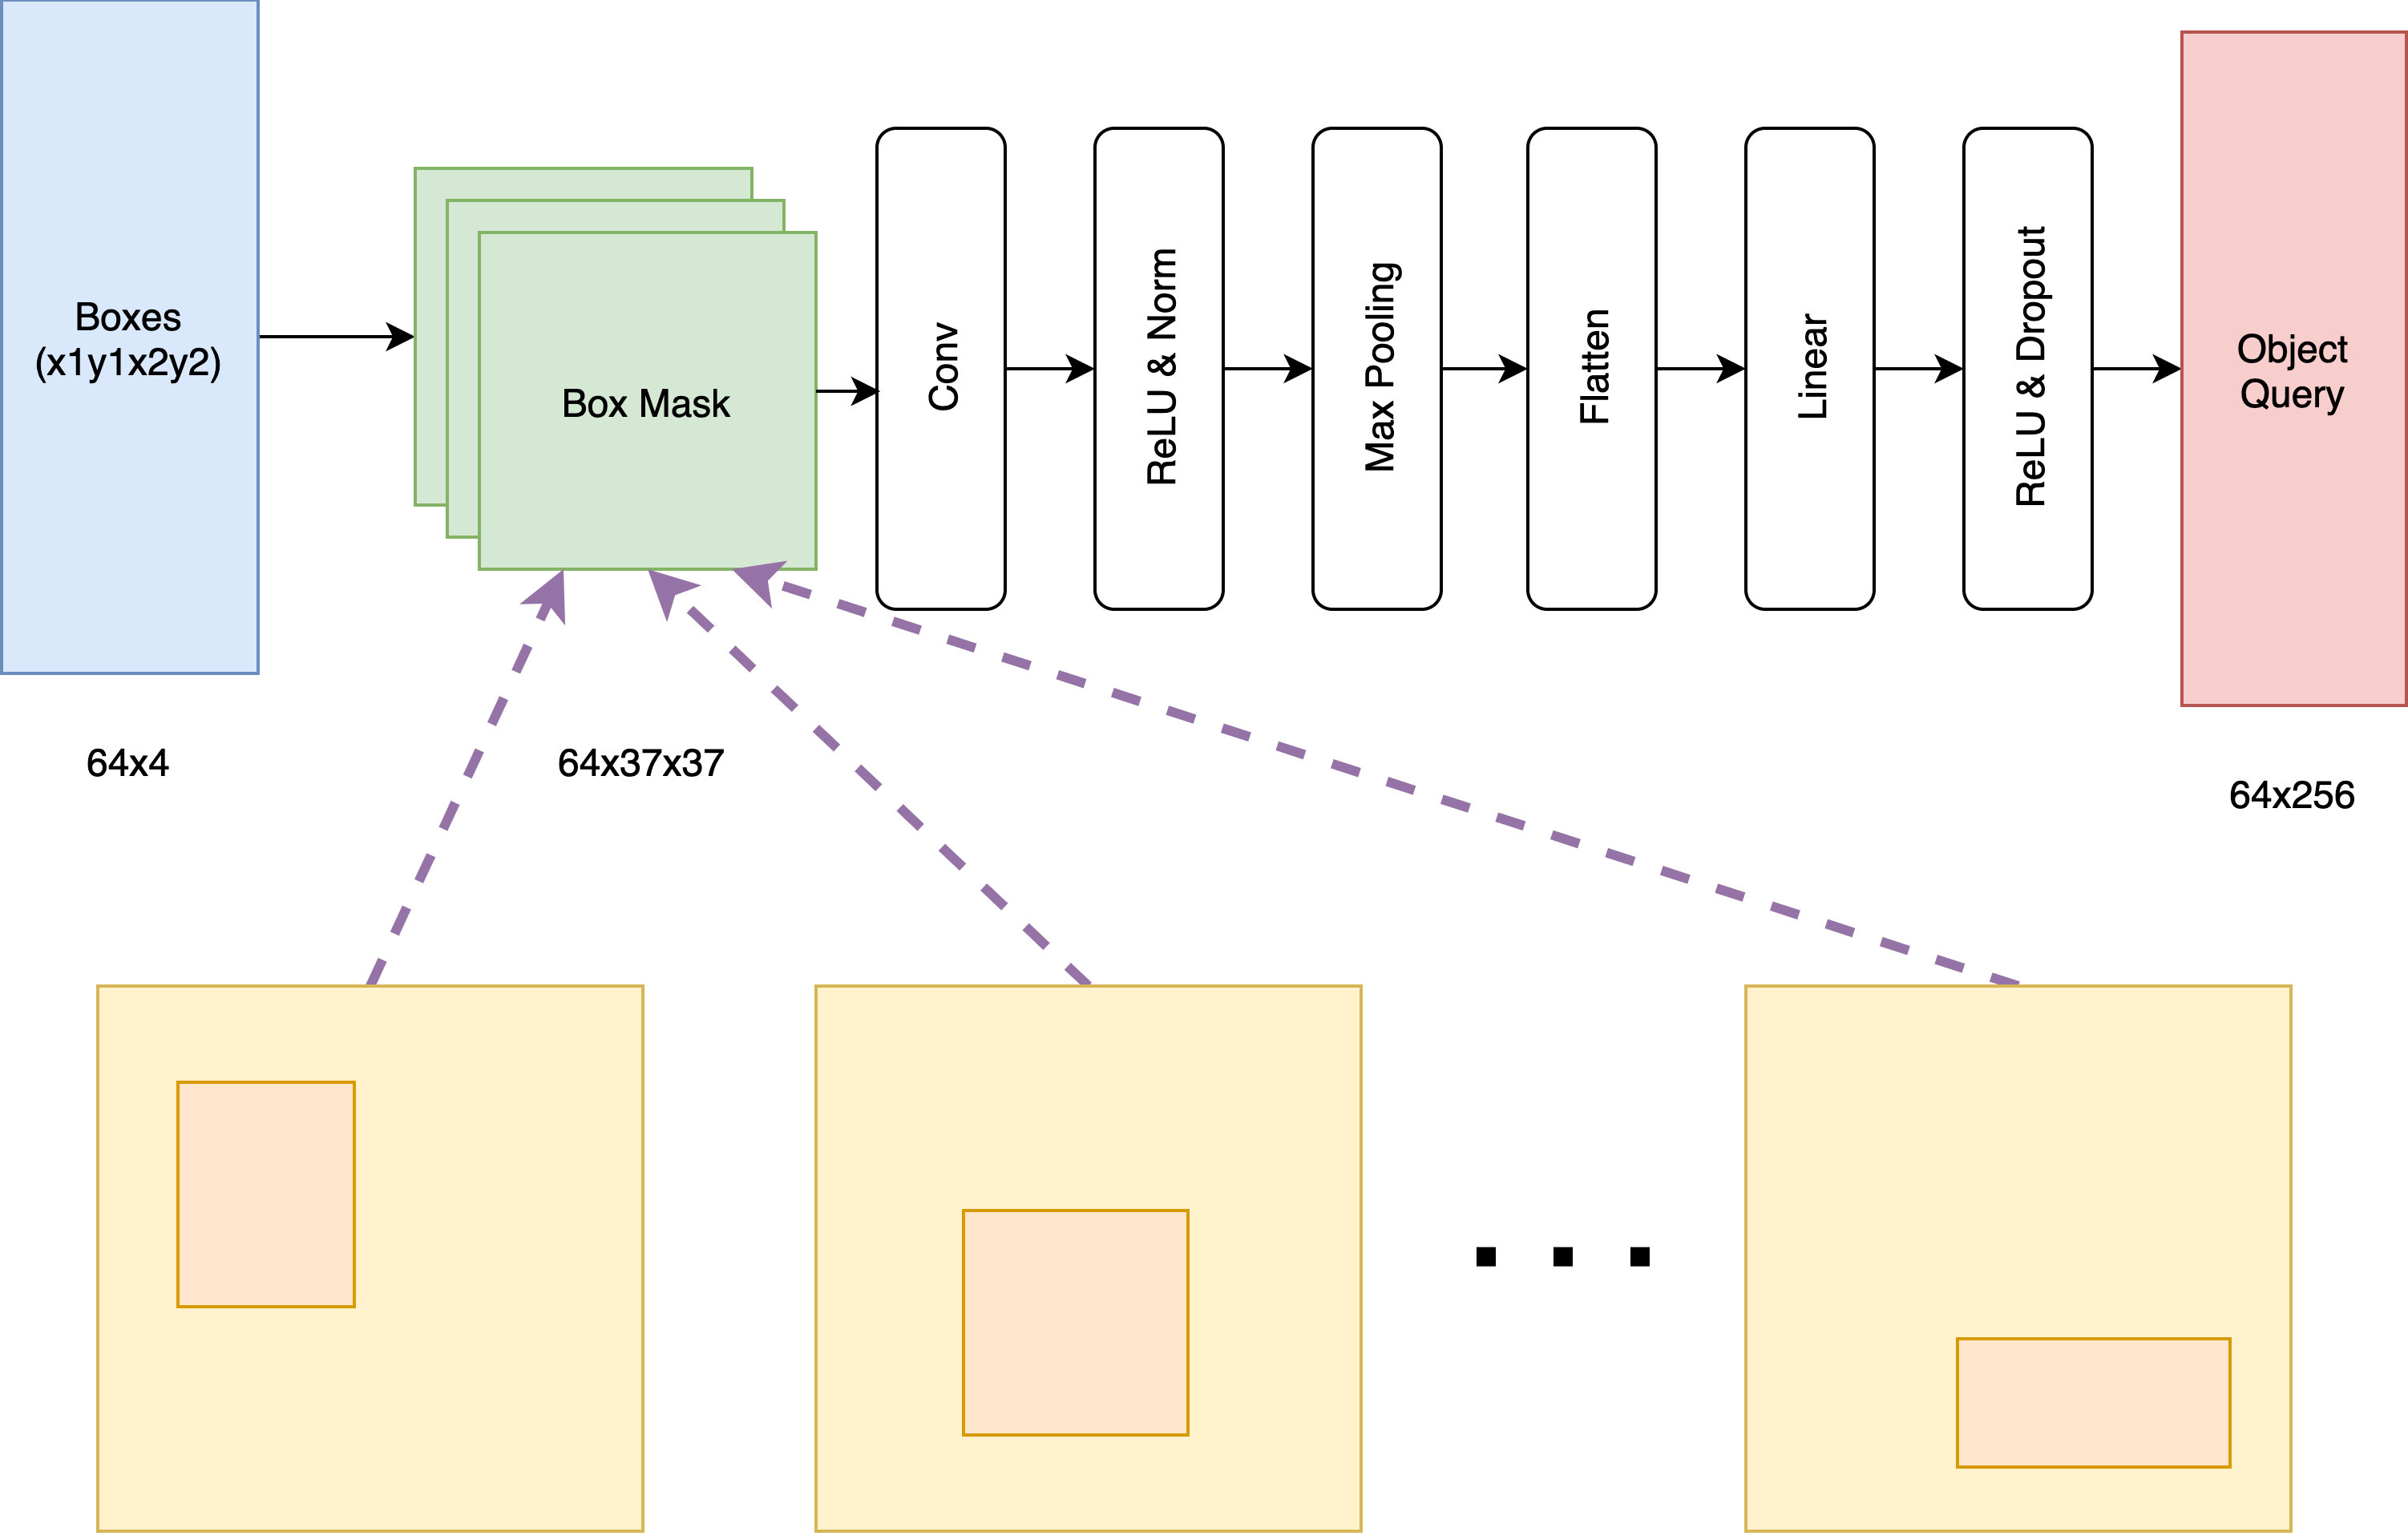
\includegraphics[width=0.8\linewidth]{figures/object_query}
	\caption[Illustration of the object query]{Illustration of the object query.}
	\label{fig:objectquery}
\end{figure}


\subsubsection{Generation of Object Feature Maps }

As shown in Figure~\ref{fig:objectquery}, we obtain the object feature through the first two Multihead Attention modules, and the process is similar to that in DETR. The difference is that we use different object queries for different tasks, as mentioned above.

For tasks PREDCLS and SGCLS, we use custom object querries. Since the query and bounding box information correspond one-to-one, the generated object features are also one-to-one correspondence, which we will prove through experiments in the next chapter.

For the task SGDET, we use a learnable query to generate the object feature, which has no corresponding relationship, and we use the Hungarian matching algorithm to find the optimal object feature with the smallest cost.

First, we obtain the predicted distributions of classes and bounding boxes through two different feed forward networks(FFN). Let us denote by $ y $ the ground truth set of objects, and $  \hat{y}= \{ \hat{y}_i\} ^N_{i=1} $ the set of $ N  $predictions.To find a bipartite matching between these two sets we search for a permutation of $ N $ elements $sigma \in \Theta _N $ with the lowest cost:
\begin{equation}\label{equ:matcher}
 \hat{\sigma} = \underset{\sigma \in \Theta _N }{argmin} \sum_{i}^{N} \mathcal L_{match} (y_i,\hat{y}_{\sigma(i)})
\end{equation}

where $\mathcal L_{match} (y_i,\hat{y}_{\sigma(i)})$ is a pair-wise matching cost between ground truth $ y_i $ and a prediction with index $ \sigma(i) $

Then we use the \textit{Hungarian loss }in DETR~\cite{carion2020end} to calculate the loss function:
\begin{equation}\label{equ:hungarianloss}
	\begin{aligned}
	&\mathcal L_{Hungarian}(y,\hat{y} ) = \sum^{N}_{i=1}[-\log{\hat{p}_{\hat{\sigma}(i)}(c_i)} + \mathbb{I}_{\{c_i \ne  \varnothing \}}\mathcal{L}_{box}(b_i,\hat{b}_{\hat{\sigma}(i)})   ], \\
	&wehre \\
	&\mathcal{L}_{box}(b_i,\hat{b}_{\hat{\sigma}(i)}) = \lambda_{iou}\mathcal{L}(b_i,\hat{b}_{\sigma(i)}) + \lambda_{L1}\left \| b_i - \hat{b}_{\sigma (i)}  \right \| _1
	\end{aligned}
\end{equation}

where $ \hat{\sigma} $ is the optimal assignment computed in the Equ.~\ref{equ:matcher}. we define probability of class $ c_i $ as $ \hat{p}_{\hat{\sigma}(i)}(c_i)$ and the predicted box as $ \hat{b}_{\sigma(i)} $. we use a linear combination of a negative log-likelihood for class prediction and a linear combination of the $  l_1  $ loss and the generalized IoU~\cite{rezatofighi2019generalized} loss for the box prediction.


\subsubsection{Object Context}

As shown in Figure~\ref{fig:objectdecoder}, we obtain the object context in the third Multihead Attention module. Its specific operation is shown in Figure~\ref{fig:objcontext}. We have given a simple example according to Equ.~\ref{equ:self_attention}. Before computing the object decoder for the first time, we initialize the object context to a tensor with 0. Assuming that we have 5 entities in the picture, before we calculate the context, the object feature size obtained from the previous calculation is $ [64, 256] $, and 59 positions will be paded by $\emptyset$. After softmax, we will Obtain a $ 64 \times 64  $ attention weight matrix (the red matrix in the figure), its meaning is the attention of each object and other objects, such as $ A_{23}$ is the attention of $ object_2 $ to $ object_3 $, and finally multiplied by the object feature we will get the object context (the yellow vector in the figure). The context of $ object_1  $is $ \sum(A_{1i}f_{obj}^i) $, that is, the context of $ object_1 $ to other $ object_i $.

\begin{figure}[tbph!]
	\centering
	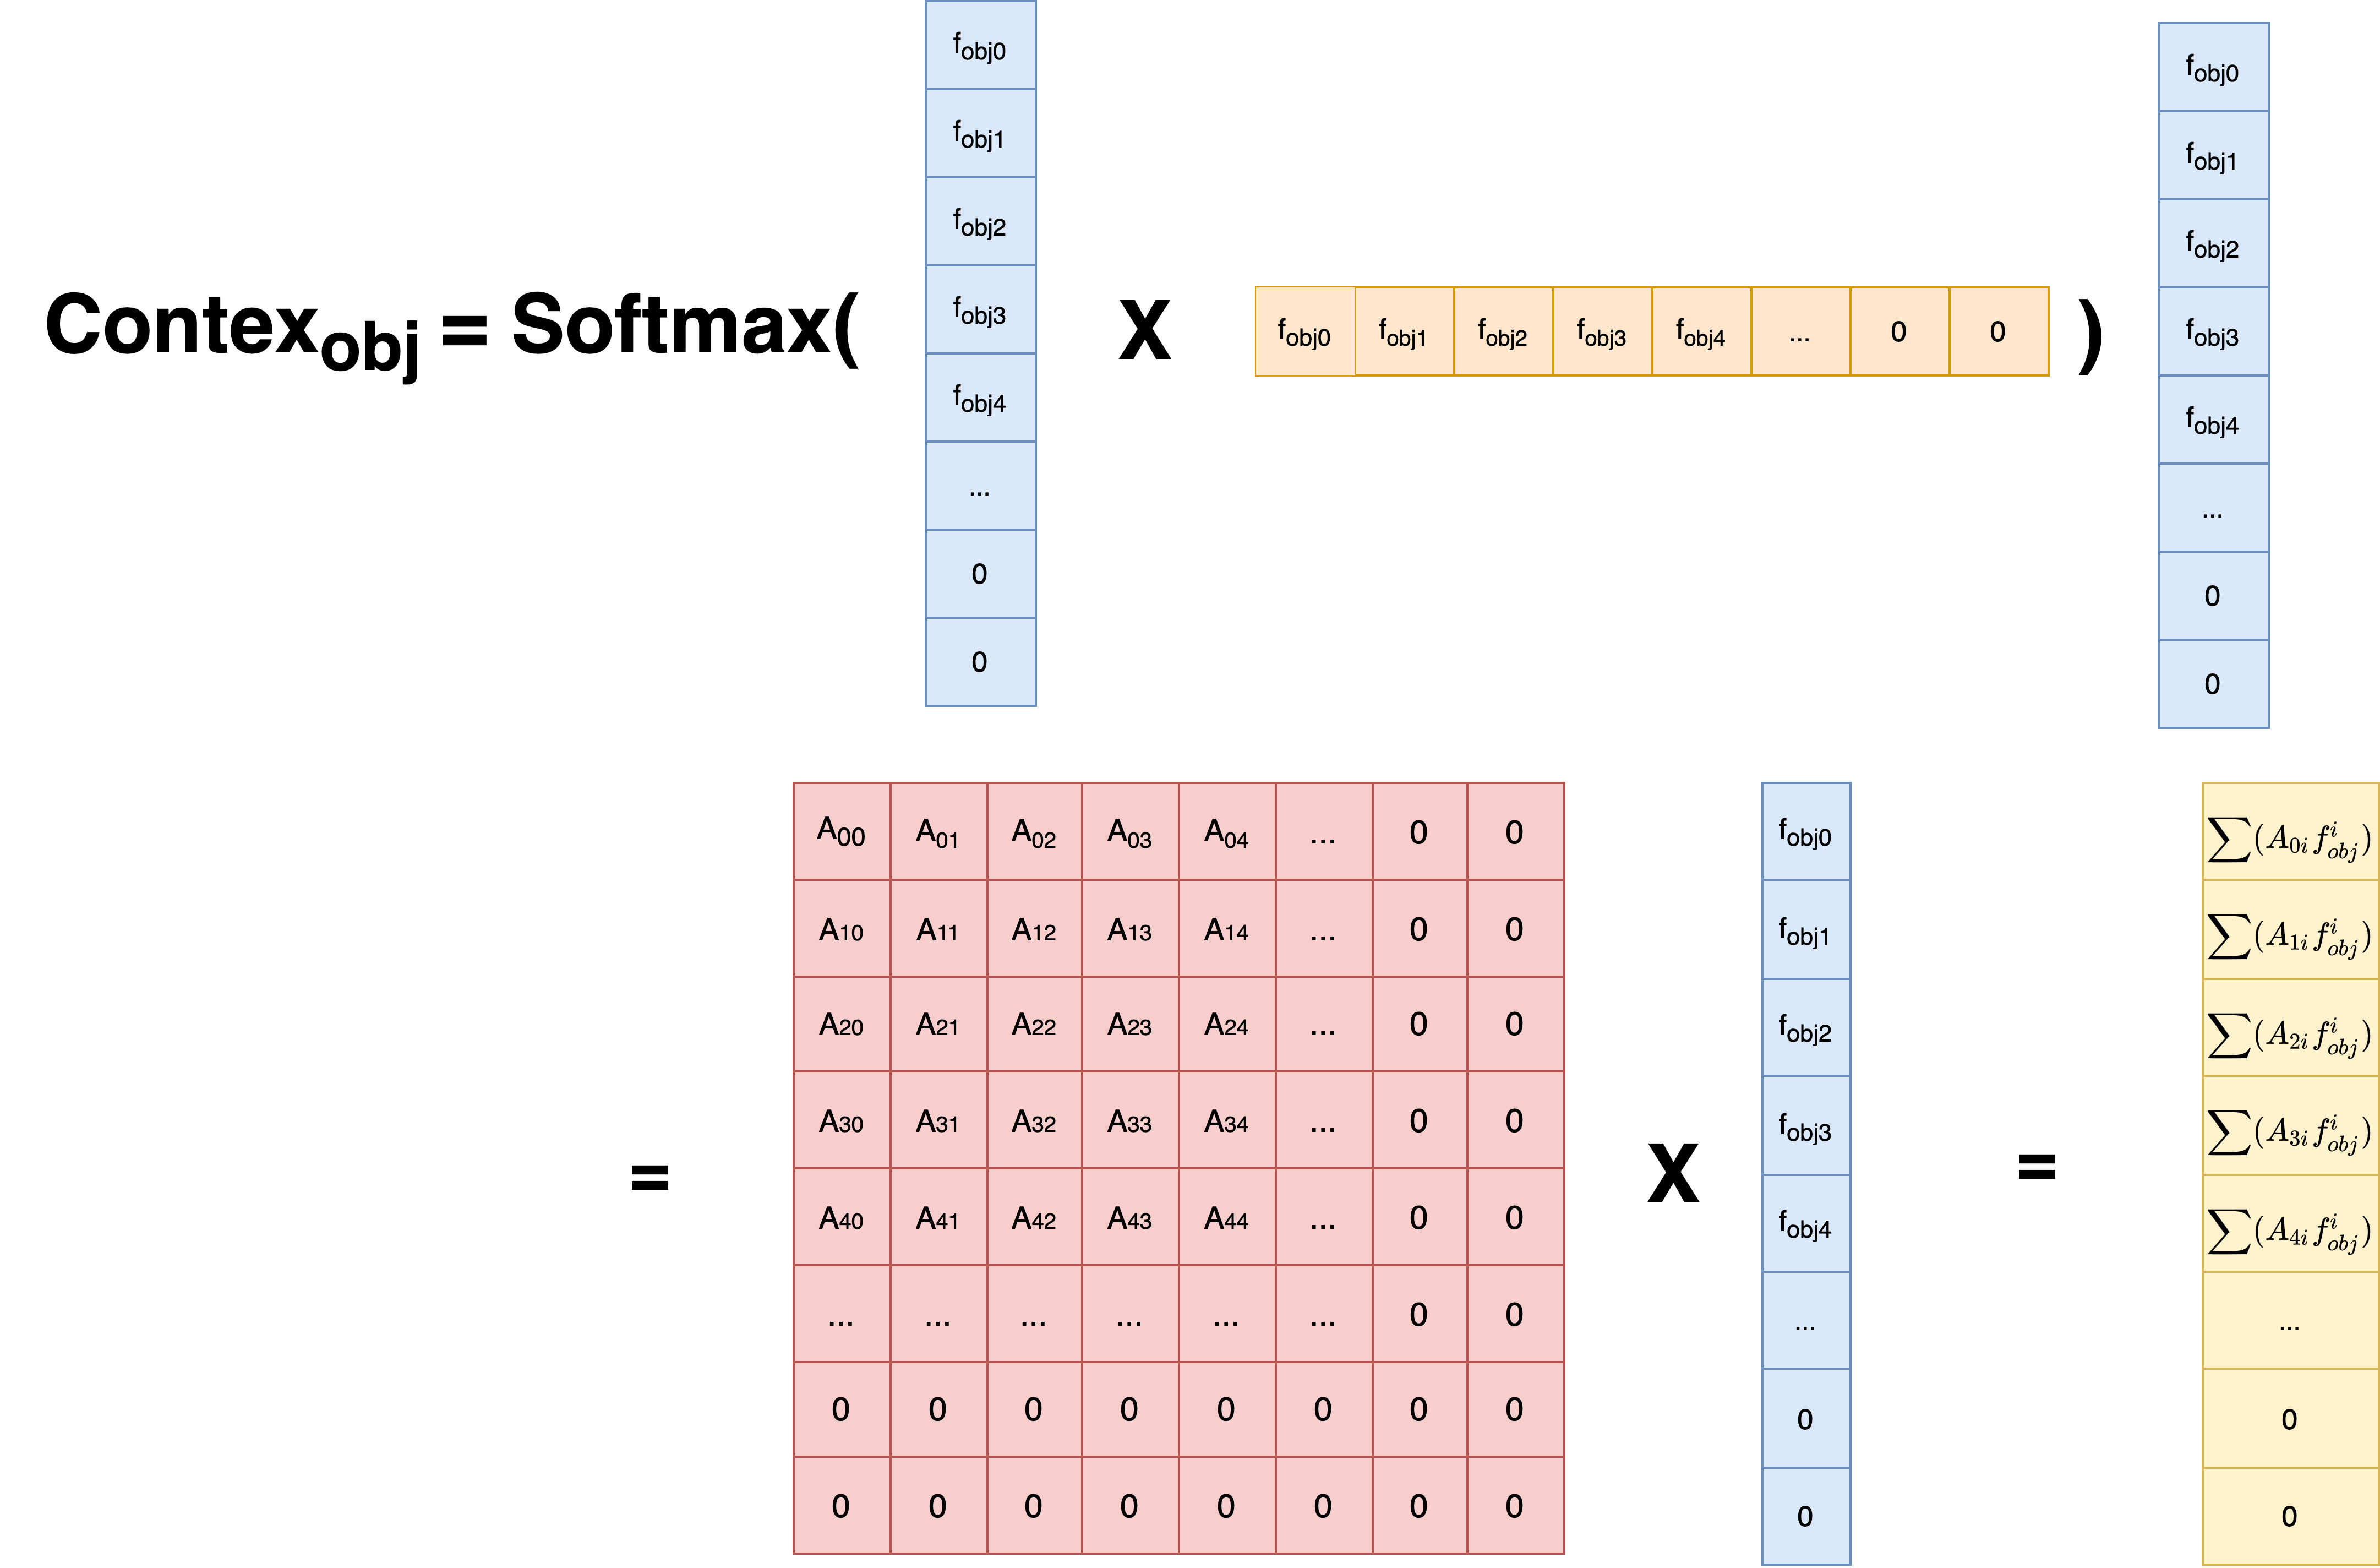
\includegraphics[width=1\linewidth]{figures/obj_context}
	\caption[A simple example of the  Object Context generation.]{A simple example of object context generation. In the first layer of decoder, we set the initial value of object context to 0. The Object Feature size is $ [64, 256] $, we assume that this picture has 5 entities, and the remaining 59 objects will be padded by 0.}
	\label{fig:objcontext}
\end{figure}


\subsection{Relation Decoder}

Our relation decoder is a typical Decoder structure consisting of two Multihead Attention modules(see in Fig.~\ref{fig:relationdecoder}). Our relationship query is customized and generated by the relationship pair $<subject,objtect>$. For example, if we have 10 entities, then we have 90 pairs, and then 90 relation queries are generated. We select the subject bounding box and object bounding box in each pair to generate two box masks, and then obtain the relation query  through the convolutional layer and the linear layer (see in Fig.~\ref{fig:relationquery}).



\begin{figure}[tbph!]
	\centering
	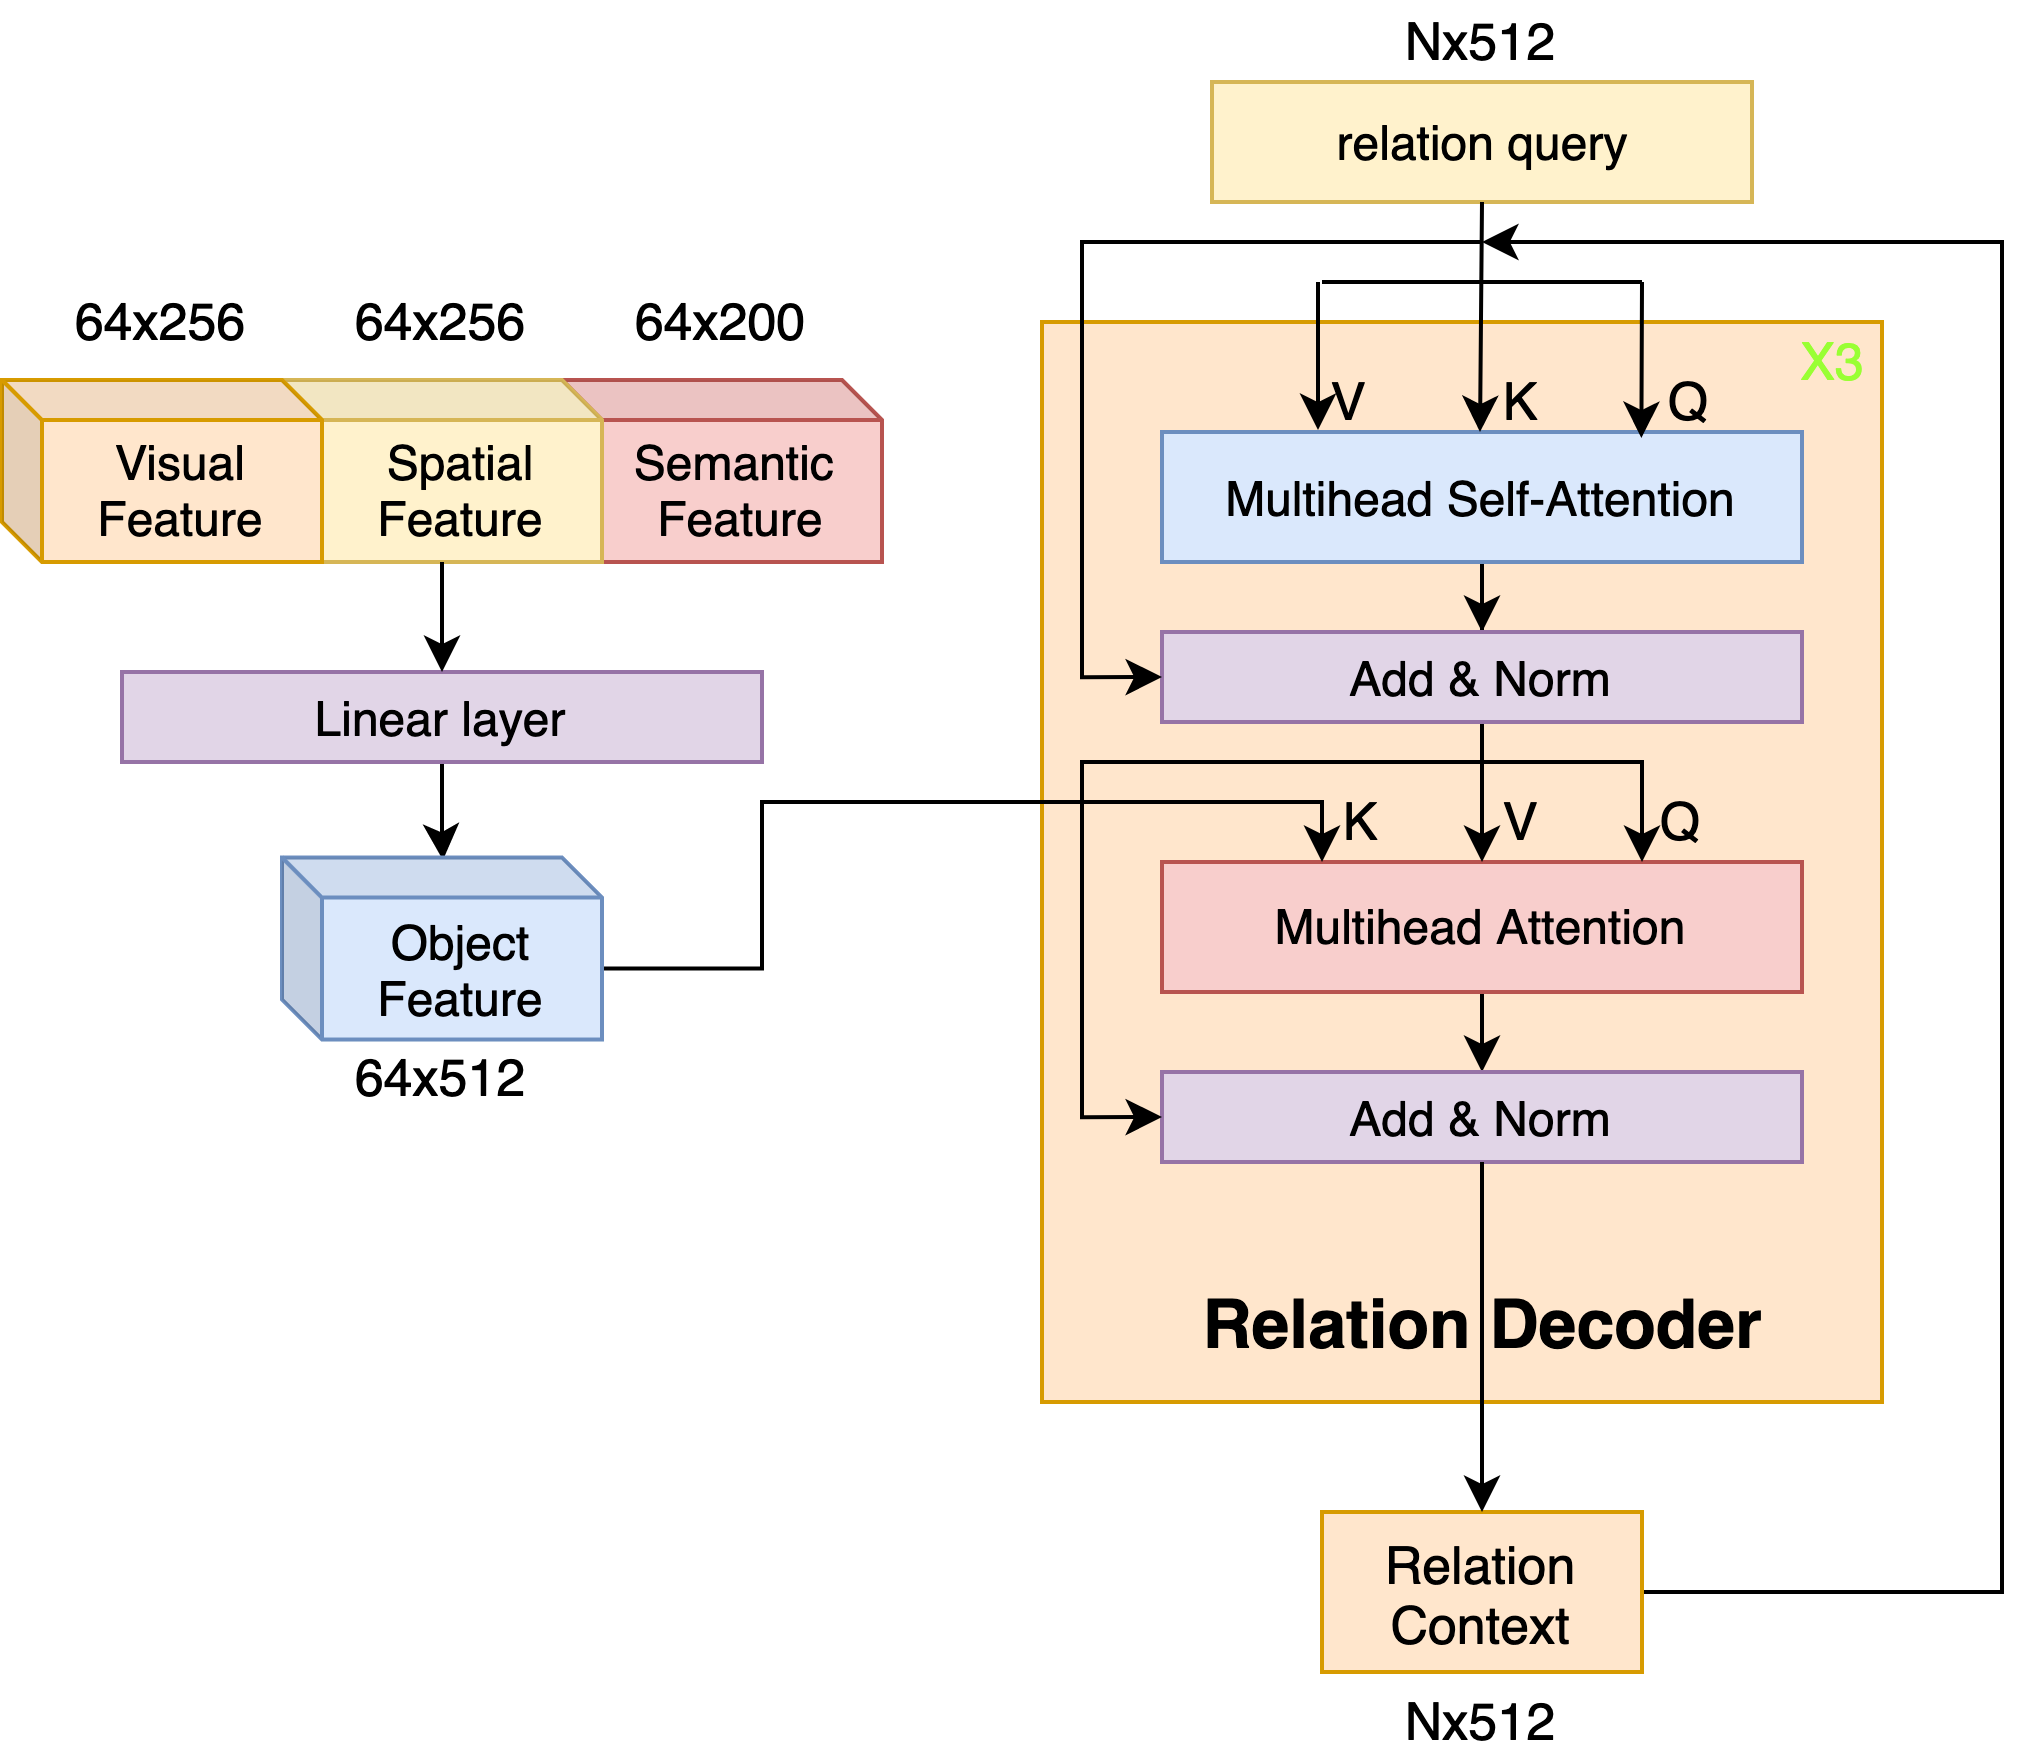
\includegraphics[width=1\linewidth]{figures/relation_decoder}
	\caption[Illustration of Relation Decoder]{Illustration of Relation Decoder.}
	\label{fig:relationdecoder}
\end{figure}

\begin{figure}[tbph!]
	\centering
	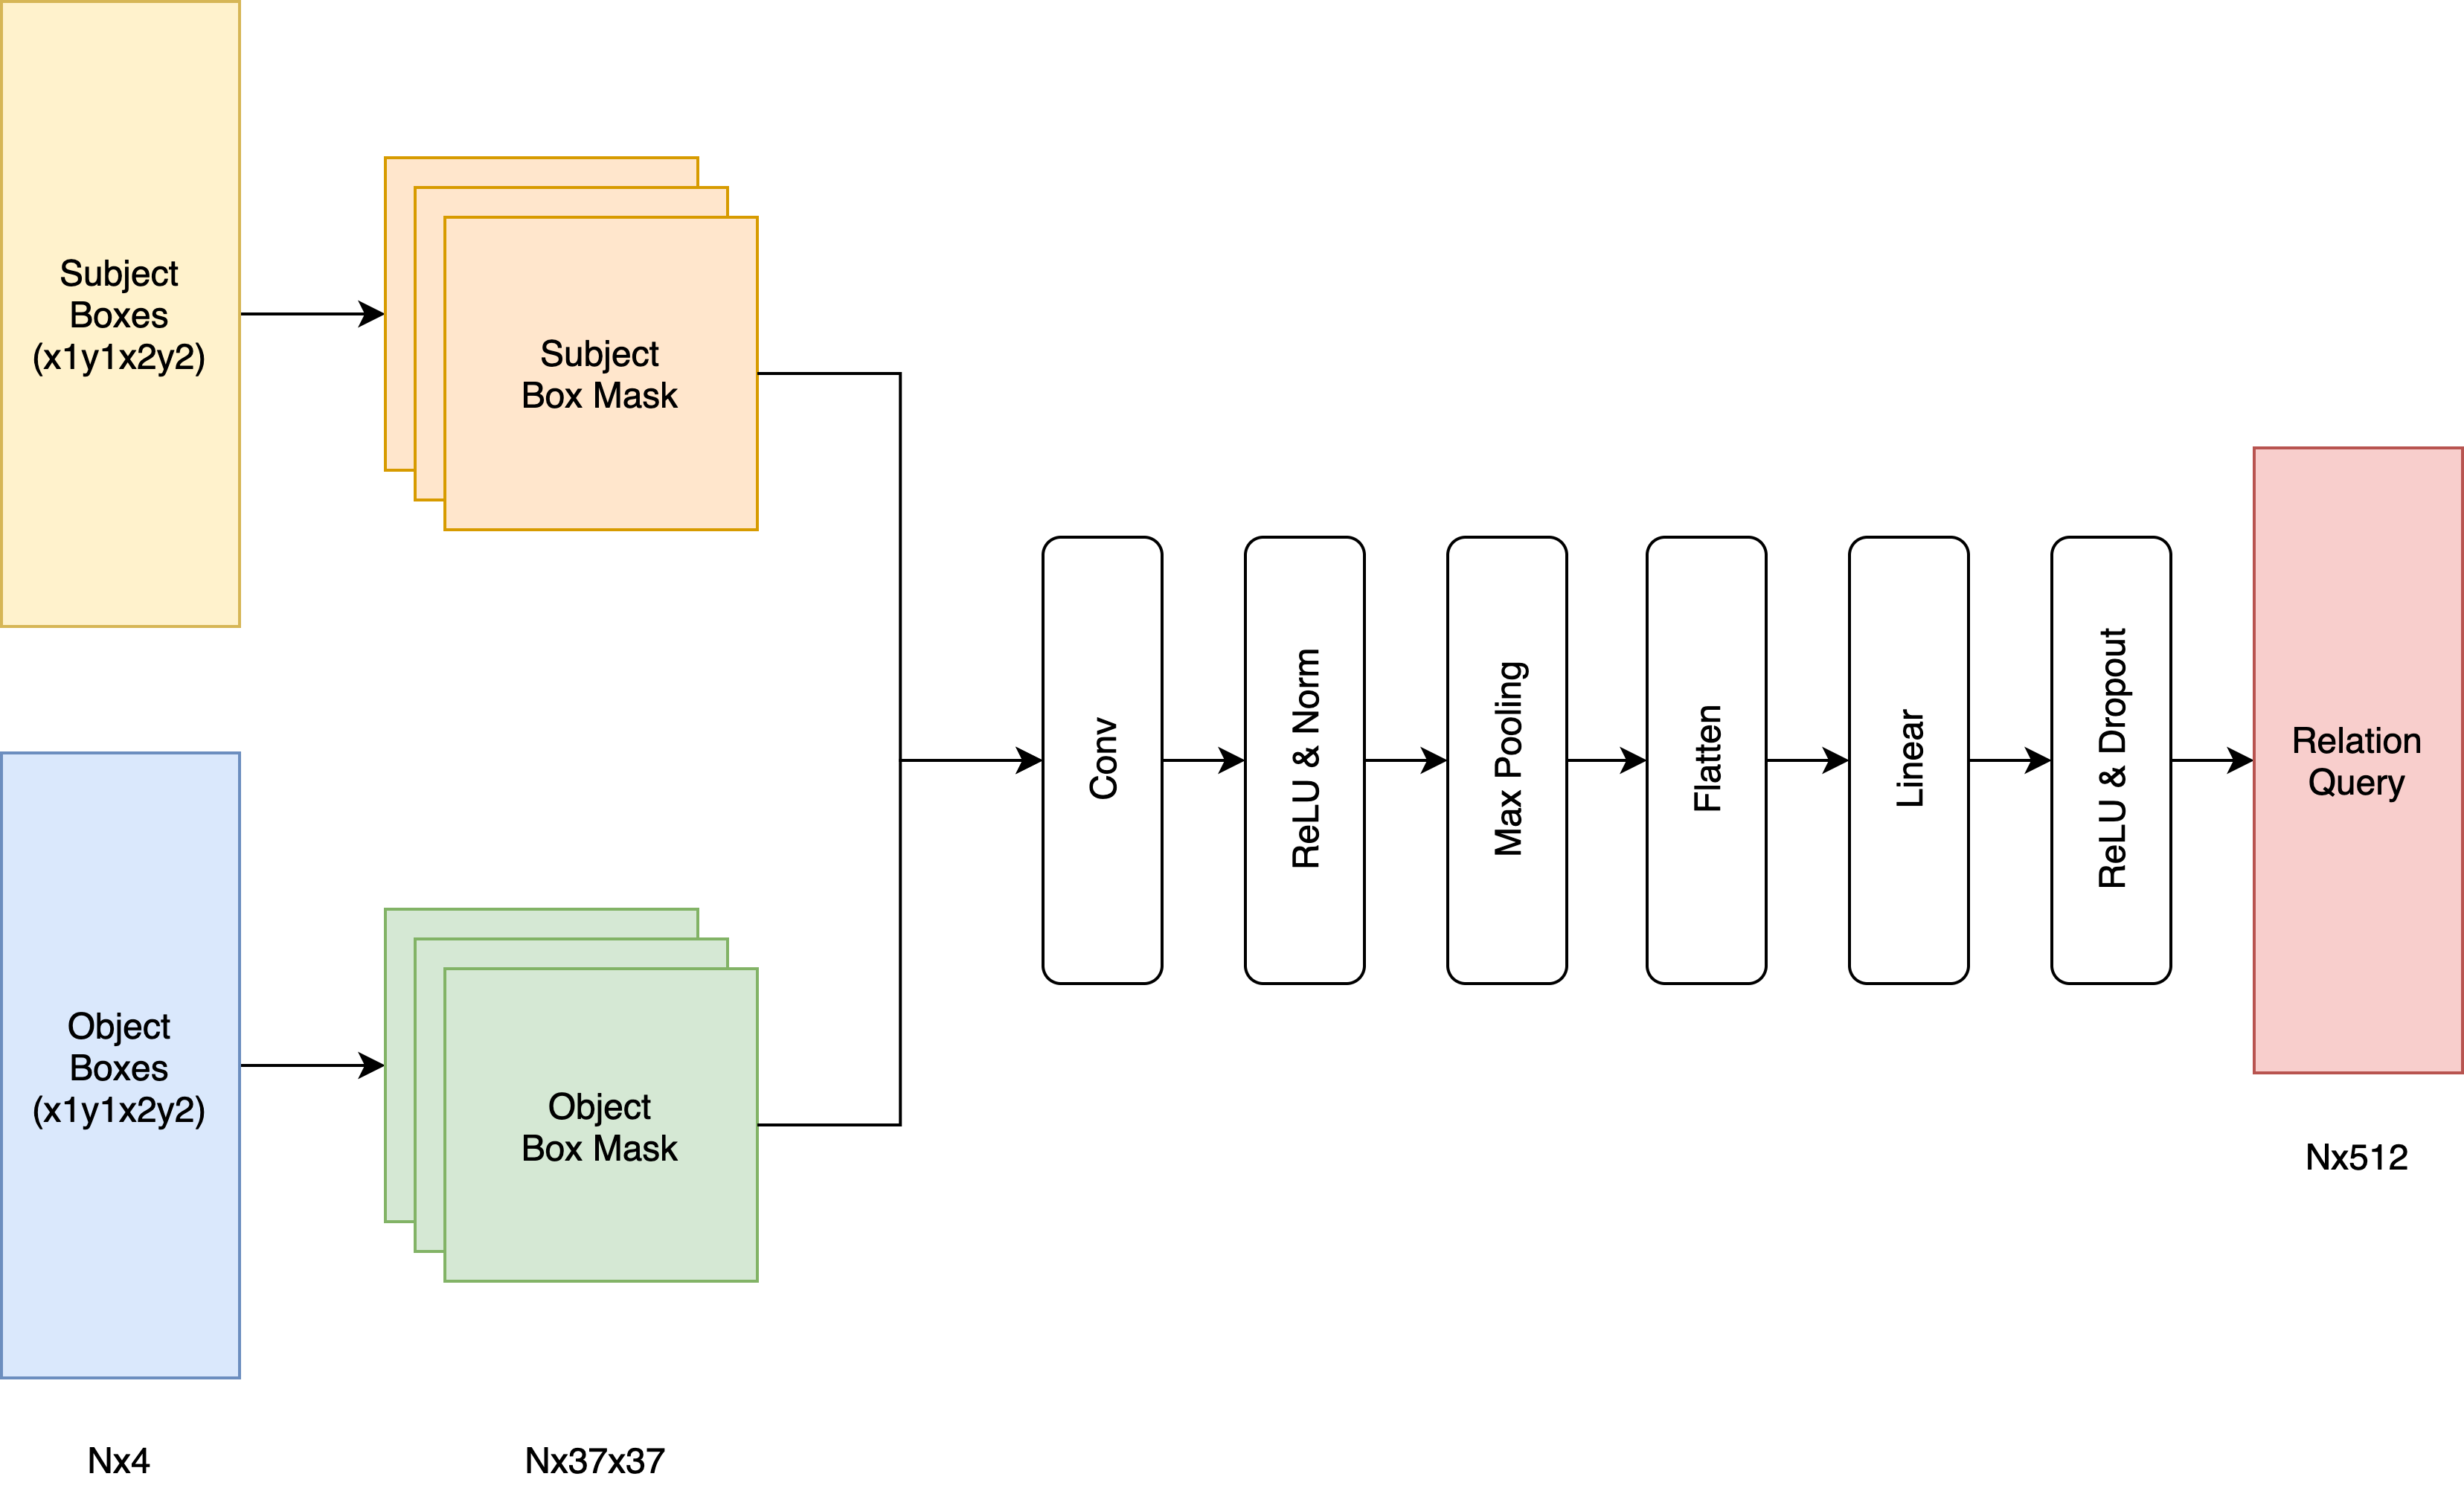
\includegraphics[width=1\linewidth]{figures/relation_query}
	\caption[Illustration of the relation query]{Illustration of the relation query. N is the number of the relation pair.}
	\label{fig:relationquery}
\end{figure}

Our relation context is the context of each relation for all objects. We use visual feat, spatial feature and  semantic feature to jointly represent object: $$f_{obj} = concat(f_{vis},f_{spt},f_{sem})$$ Among them, the visual feature $f_{vis}$ is the object feature obtained through the object decoder. The semantic feature $ f_{sem} $ is a tensor containing the semantic information of entities obtained by encoding the category through GloVe~\cite{pennington2014glove}. The spatial feature $ f_{spt} $ is a feature that contains the spatial location information of the entity. We can get it through the bounding box. In our thesis, the attention map obtained in the object decoder also has good spatial location information, so we also use the extraction of the attention map to obtain the spatial feature.



\subsection{Predicate Classifier}
Predicate prediction is a very important task in VRD problems. We get the features and context from the previous module to predict the predicate, as shown in Figure~\ref{fig:predicateclassifer}. The calculation process is shown in the following equation:

$$ score_{pred}(i,j) = Linear(concat(feat_{obj}^i, context_{rel}^{ij}, context_{obj}^i, feat_{obj}^j) $$

where $ i $ is the index of subject, $ j $ is the index of object,  $ feat_{obj} $ is the visual feature obtained from the Object Decoder, so $ feat_{obj}^i $ is the visual feature of the subject, and the $ feat_{obj}^j $ is the visual feature of the object. $ context_{rel}^{ij} $ is the relation context of the realtion $ pair(subject_i,object_j)  $obtained from the Relation Decoder, $  context_{obj}^i $ is the object context of the $subject_i$ obtained from the Object Decoder.

 \begin{figure}[tbph!]
 	\centering
 	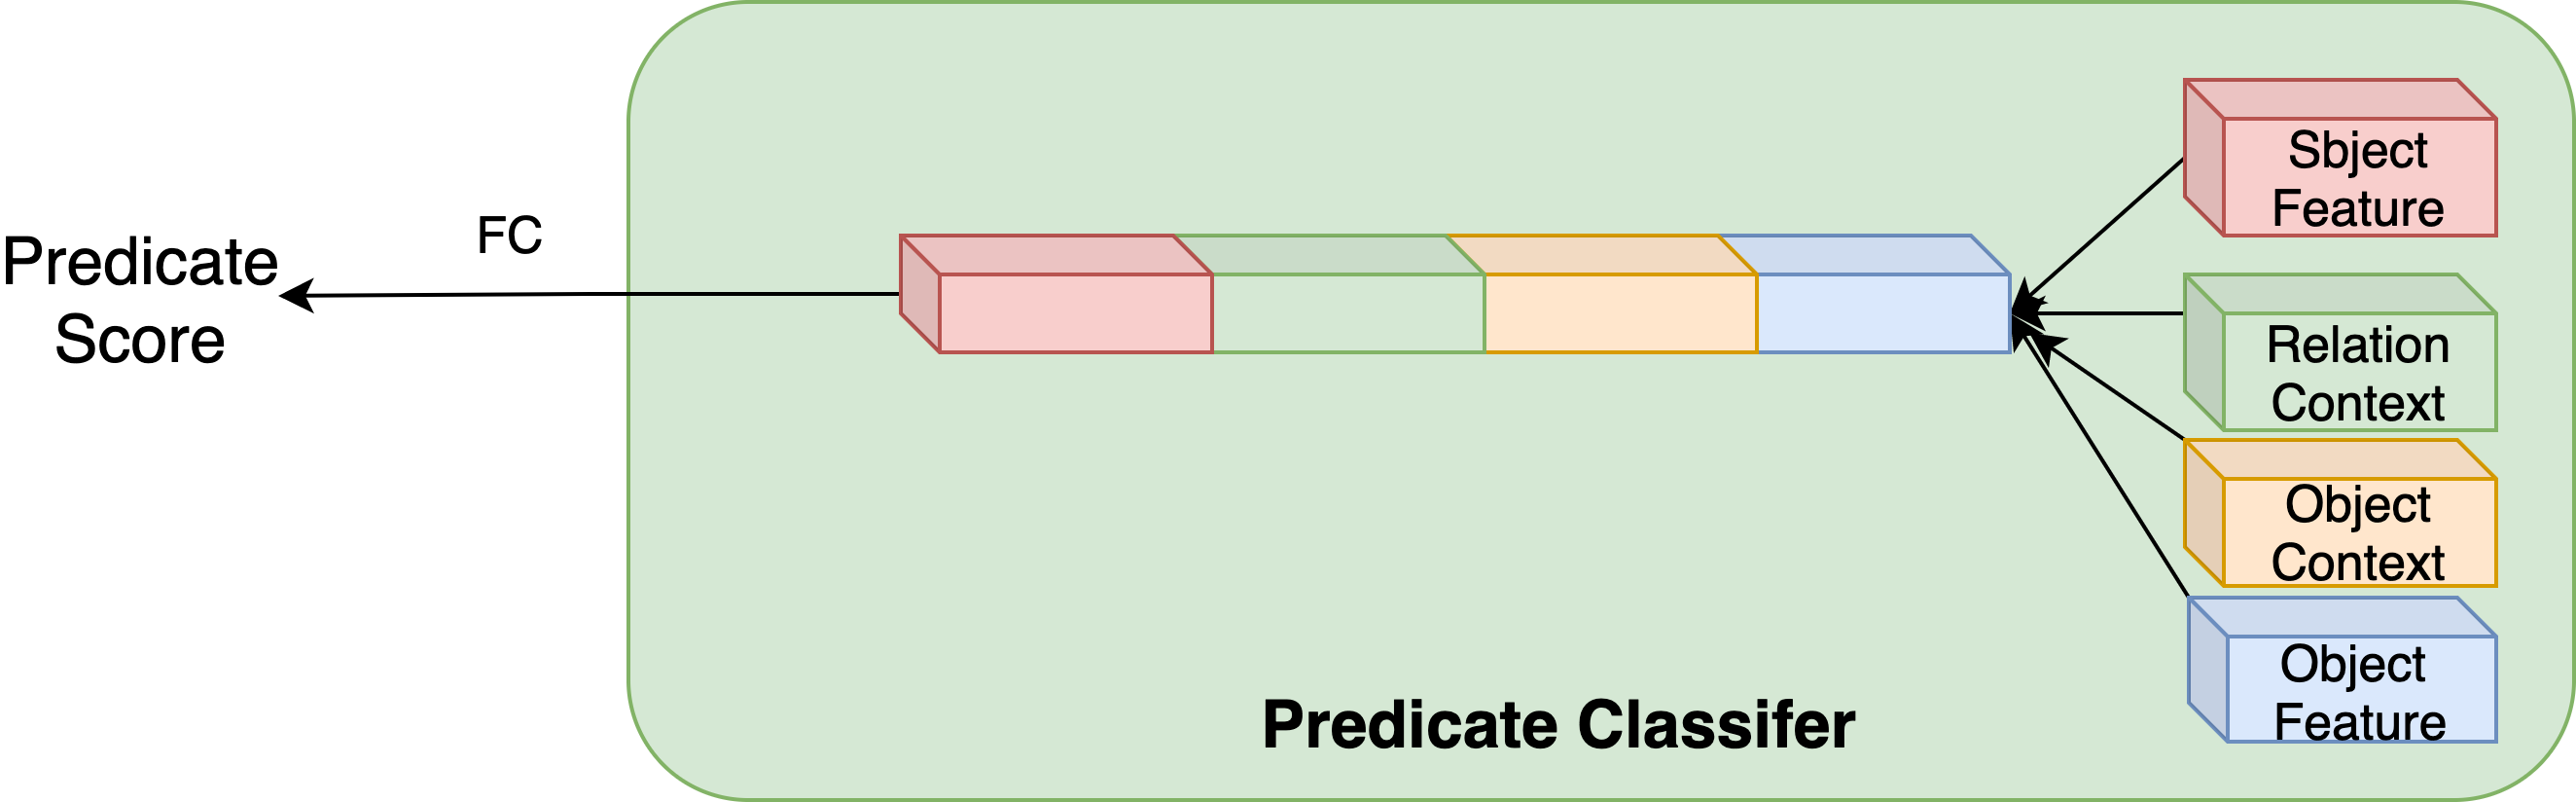
\includegraphics[width=1\linewidth]{figures/predicate_classifer}
 	\caption[Illustration of the predicate classfier]{Illustration of the predicate classfier.}
 	\label{fig:predicateclassifer}
 \end{figure}
 
 
 \begin{figure}[h]
 	\centering
 	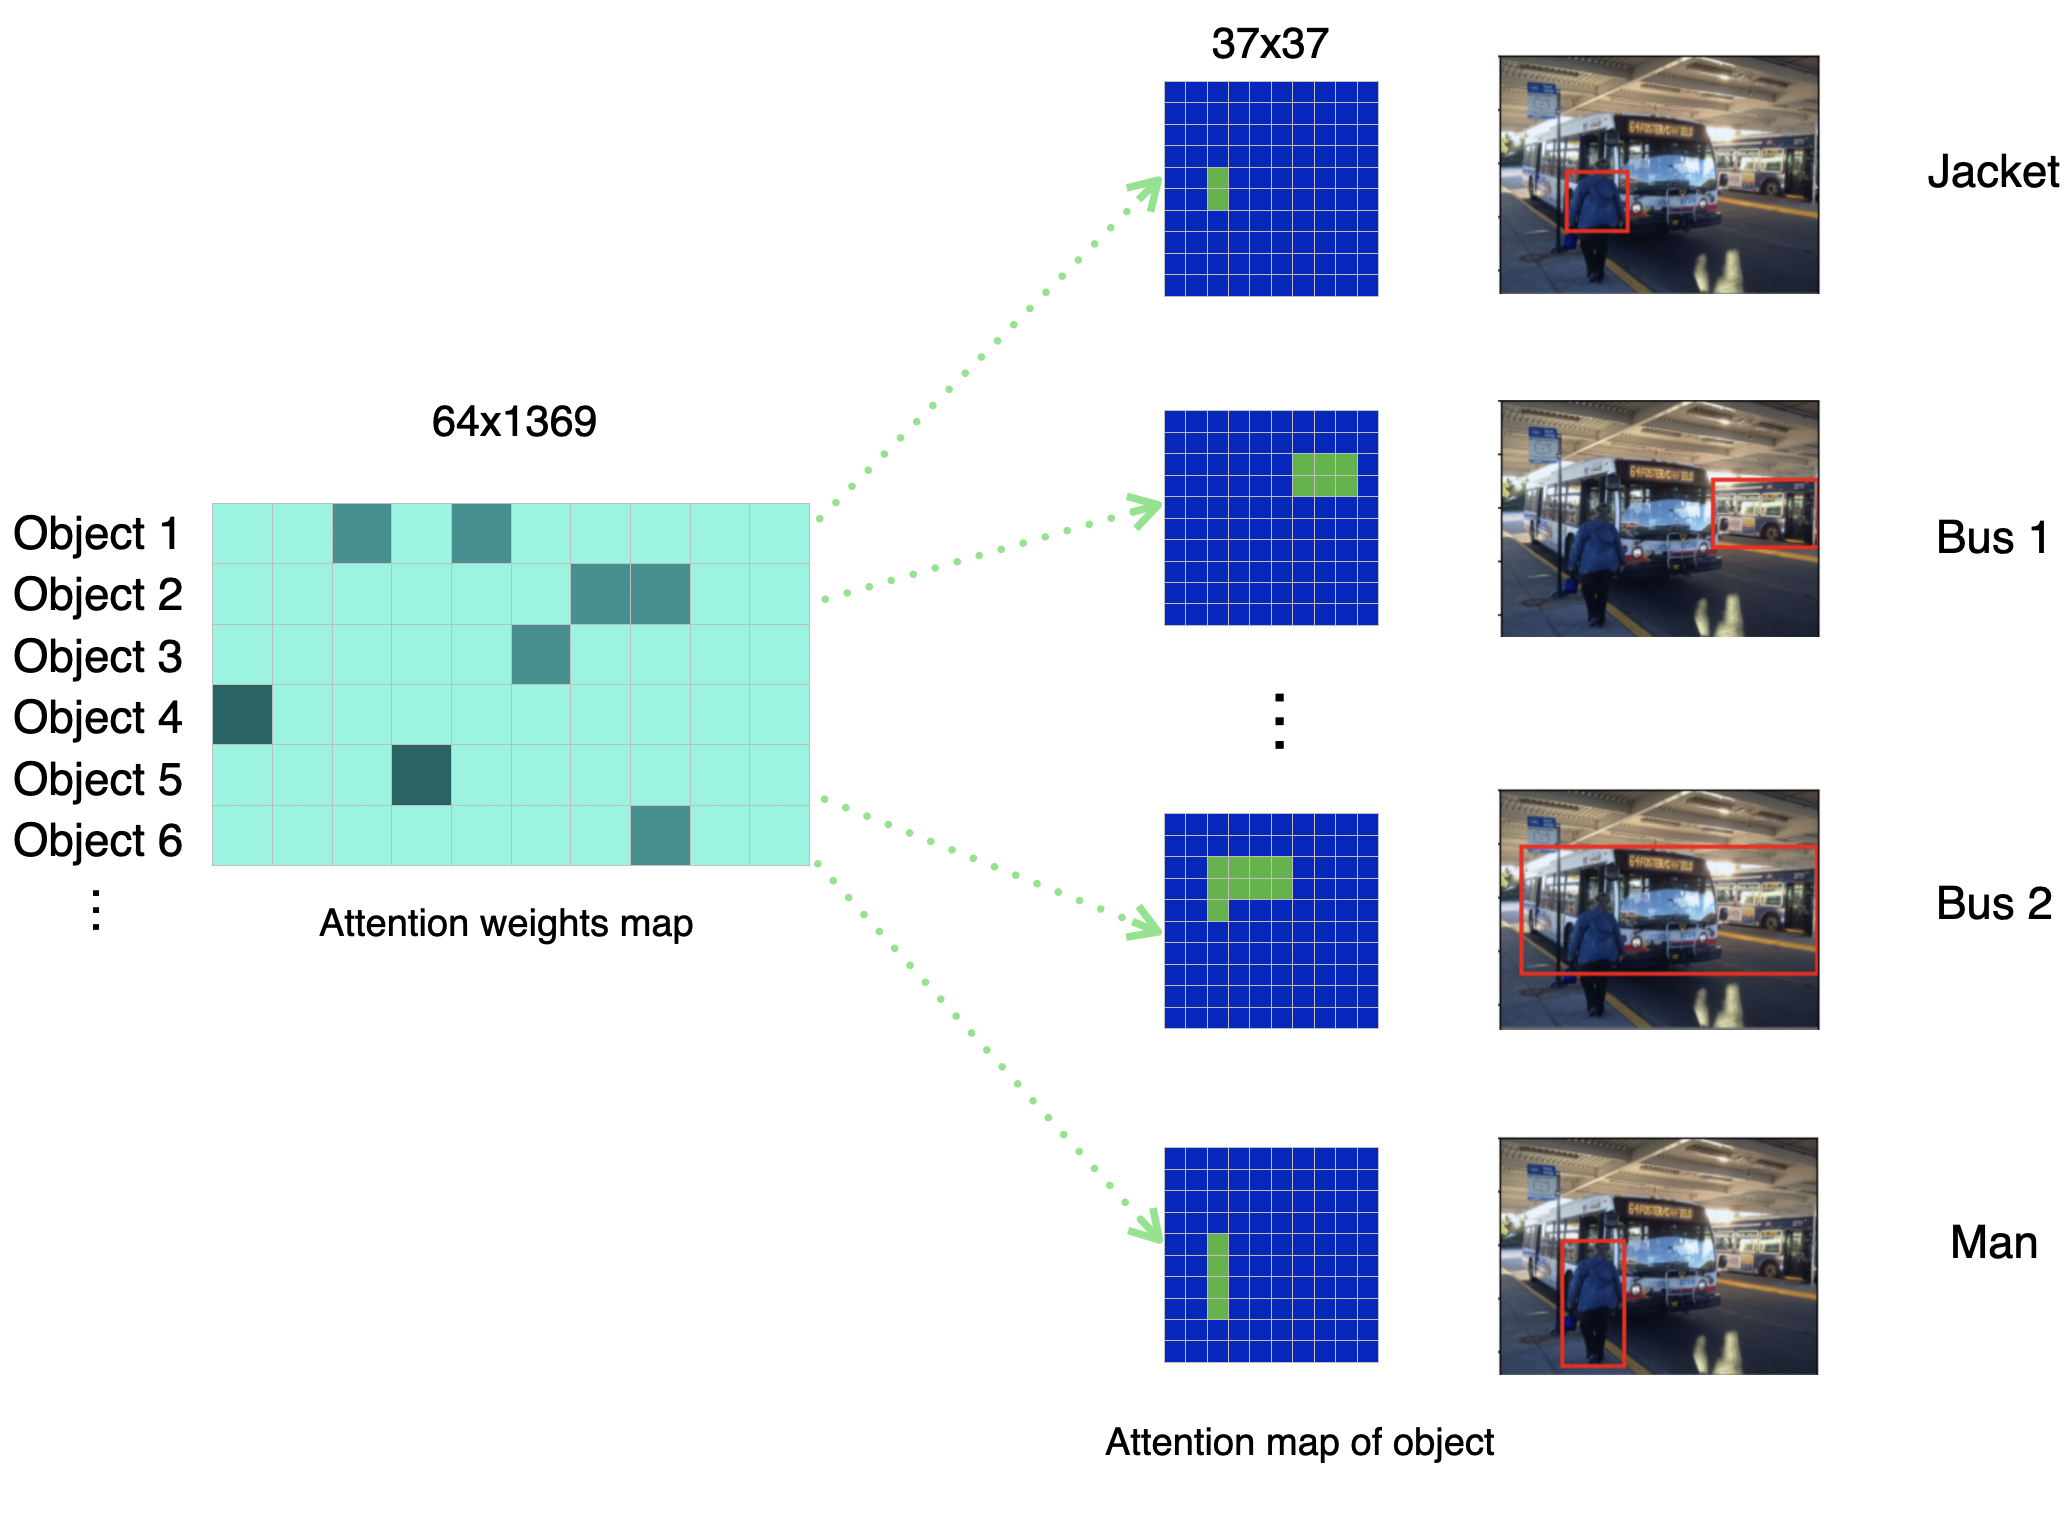
\includegraphics[width=0.8\linewidth]{figures/attention_map}
 	\caption[Illustration of the attention map]{Each row in the attention weights map represents the attention of each object. }
 	\label{fig:attentionmap}
 \end{figure}
 

\subsection{Attention Loss}

In the object decoder(see in Fig.~\ref{fig:objectdecoder}), we obtain the object visual feature through the second Multihead Attention module, and the attention maps size of $ [64, 1369] $. We can convert it to a tensor of $ [64, 37, 37], $ which means the attention weights of each object to each pixel in the image feature from the encoder.



As shown in Fig.~\ref{fig:attentionmap}, we get an attention weights map of size 64x1369, and each row of it can be transformed into a small attention map of 37x37 size. We hope that this attention map can have a spatial correspondence with the entity in the picture. For example, in this picture we can see a man wearing a purple jacket and two buses. We hope to find the corresponding object in the small attention map, we will find green in the attention map of the jacket. The attention weight of the part is much higher than the blue one. This shows that we pay more attention to this green area when generating the object feature of the jacket. In this way, we can better visualize the object and make our object feature better.

Therefore, we designed an attention loss according to the ranking loss, so that the attention weights of the green area are higher than that of the blue area:

\begin{equation}
	loss_{attention}=max(0, \frac{1}{m}\sum_{m}Att_j^{no\_obj}-\frac{1}{n}\sum_{n}Att_i^{obj}+0.25
	/1369)
\end{equation}

where $Att_j^{no\_obj}$ is the attention value $  j  $ of the the area outside the bounding box  of  object, $ m $ is the total number of attention values. $ Att_i^{obj} $ is the attention value $  i  $ of the the area within the bounding box  of object, $ n $ is the total number of attention values. Then $ Margin=0.25/1369  $ is quarter the average of the attention map.


\chapter{Experimental Results}
\label{chap:experiment}
In this Chapter we evaluate our method on three real-world surveillance video benchmark datasets and analyze the experimental results in detail. Furthermore, we will compare our model with others popular approaches.

\begin{figure}[!htbp]
	\renewcommand{\thesubfigure}{\arabic{subfigure}}
	%\renewcommand{\thefigure}{\arabic{figure}}
	\makeatletter
	\renewcommand{\@thesubfigure}{(\thesubfigure)\space}
	\renewcommand{\p@subfigure}{\thefigure.}
	\makeatother
	\centering
	\subfigure[16.6\%]{
		\label{fig:subfigure:1}
		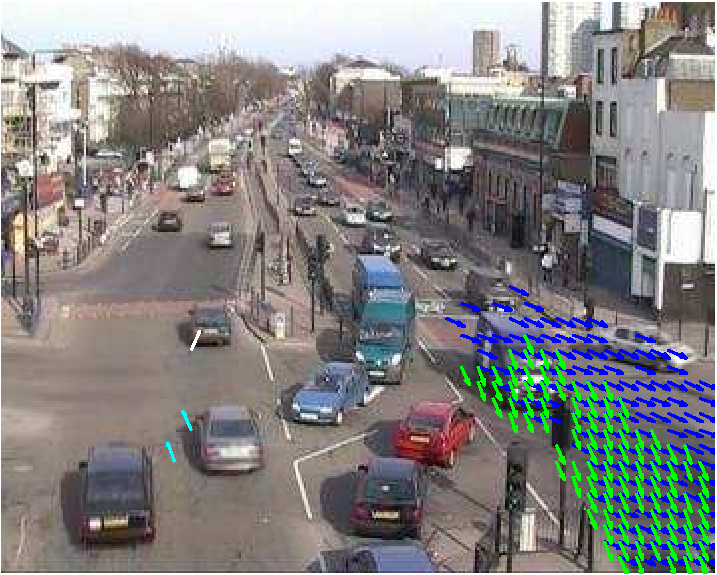
\includegraphics[width=3.7cm, height=2.5cm]{figures/qmul/t1-crop.pdf}}
	\subfigure[15.9\%]{
		\label{fig:subfigure:2}
		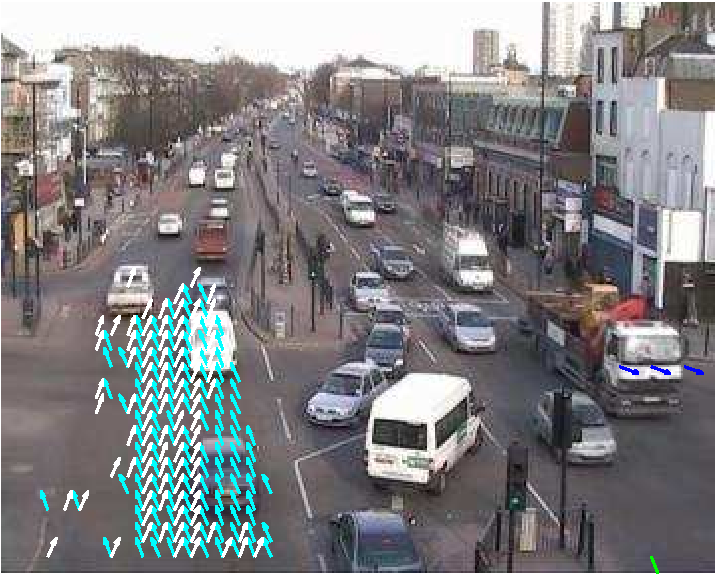
\includegraphics[width=3.7cm, height=2.5cm]{figures/qmul/t2-crop.pdf}}
	\subfigure[15.8\%]{
		\label{fig:subfigure:3}
		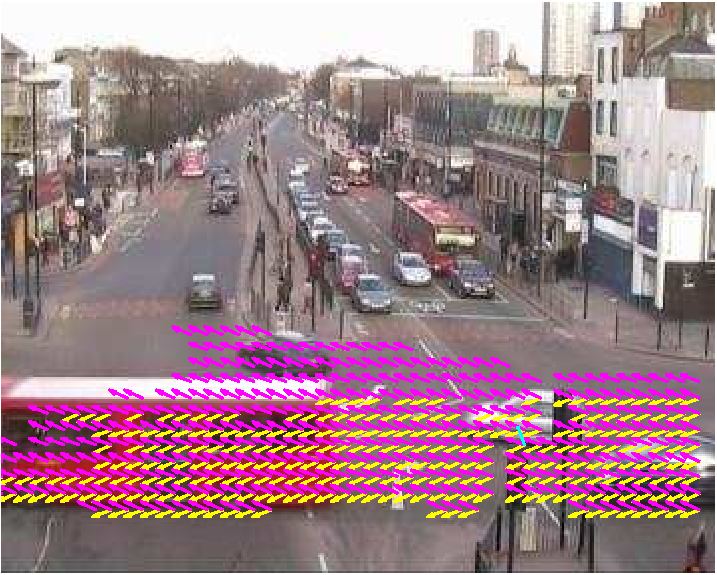
\includegraphics[width=3.7cm, height=2.5cm]{figures/qmul/t3-crop.pdf}}
	\subfigure[9.8\%]{
		\label{fig:subfigure:4}
		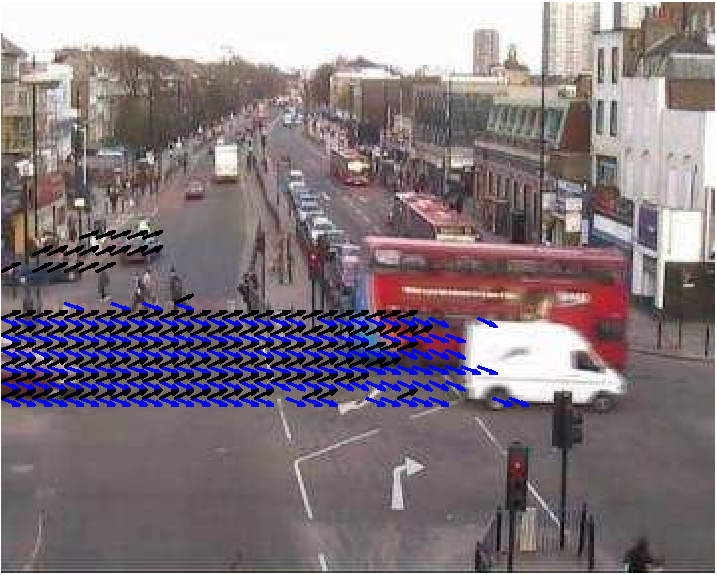
\includegraphics[width=3.7cm, height=2.5cm]{figures/qmul/t4-crop.pdf}}
	\subfigure[6.2\%]{
		\label{fig:subfigure:5}
		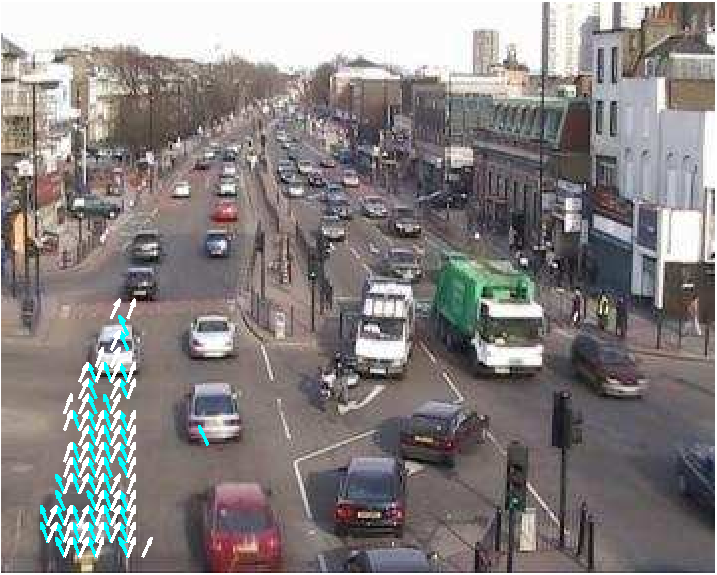
\includegraphics[width=3.7cm, height=2.5cm]{figures/qmul/t5-crop.pdf}}
	\subfigure[5.7\%]{
		\label{fig:subfigure:6}
		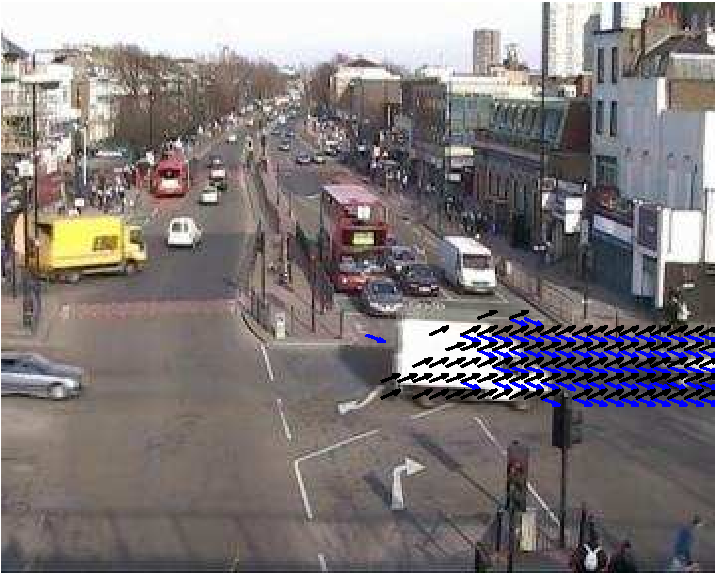
\includegraphics[width=3.7cm, height=2.5cm]{figures/qmul/t6-crop.pdf}}
	\subfigure[3.5\%]{
		\label{fig:subfigure:7}
		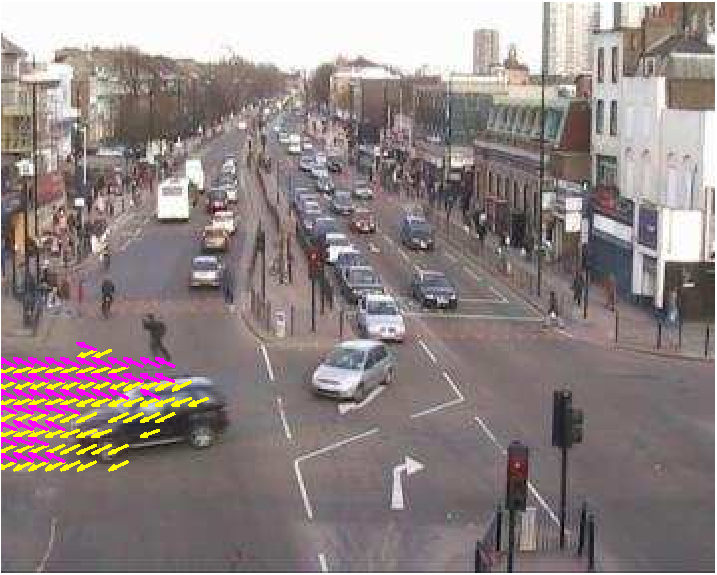
\includegraphics[width=3.7cm, height=2.5cm]{figures/qmul/t7-crop.pdf}}
	\subfigure[3\%]{
		\label{fig:subfigure:8}
		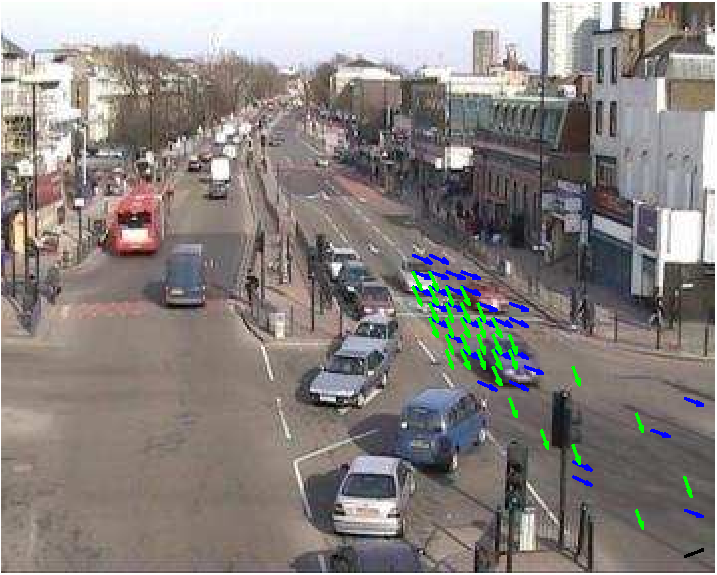
\includegraphics[width=3.7cm, height=2.5cm]{figures/qmul/t8-crop.pdf}}
	\subfigure[2.7\%]{
		\label{fig:subfigure:9}
		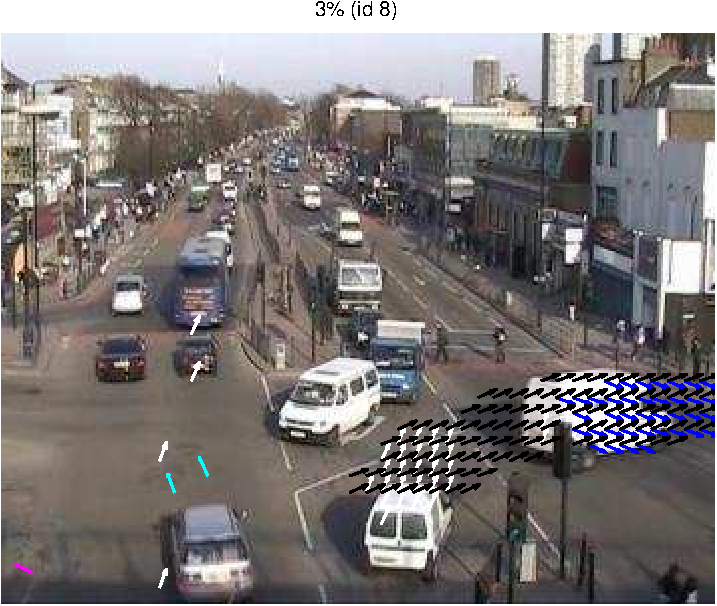
\includegraphics[width=3.7cm, height=2.5cm]{figures/qmul/t9-crop.pdf}}
	\subfigure[2.7\%]{
		\label{fig:subfigure:10}
		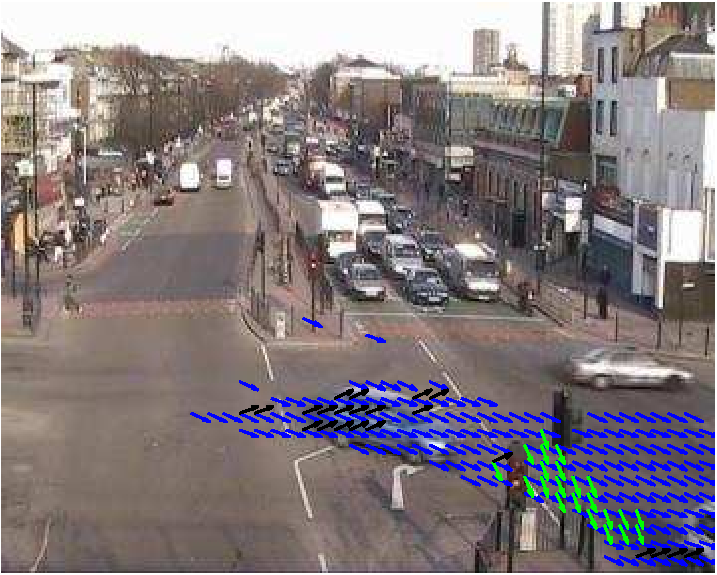
\includegraphics[width=3.7cm, height=2.5cm]{figures/qmul/t10-crop.pdf}}
	\subfigure[2.5\%]{
		\label{fig:subfigure:11}
		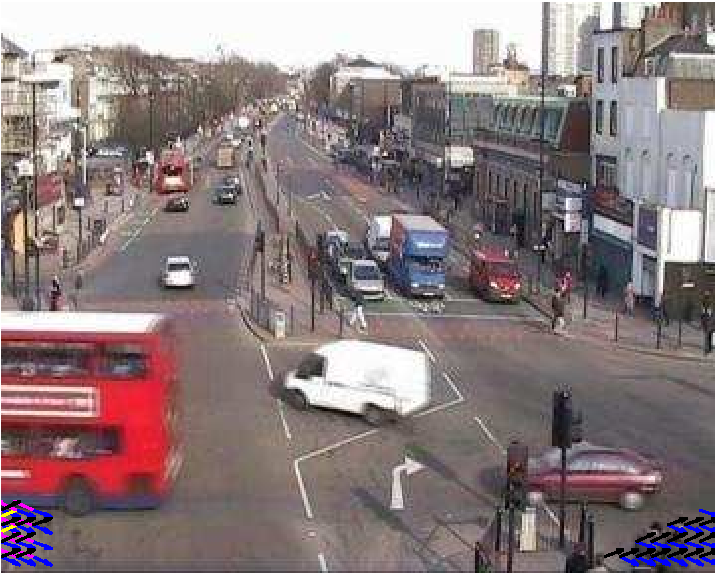
\includegraphics[width=3.7cm, height=2.5cm]{figures/qmul/t11-crop.pdf}}
	\subfigure[1.9\%]{
		\label{fig:subfigure:12}
		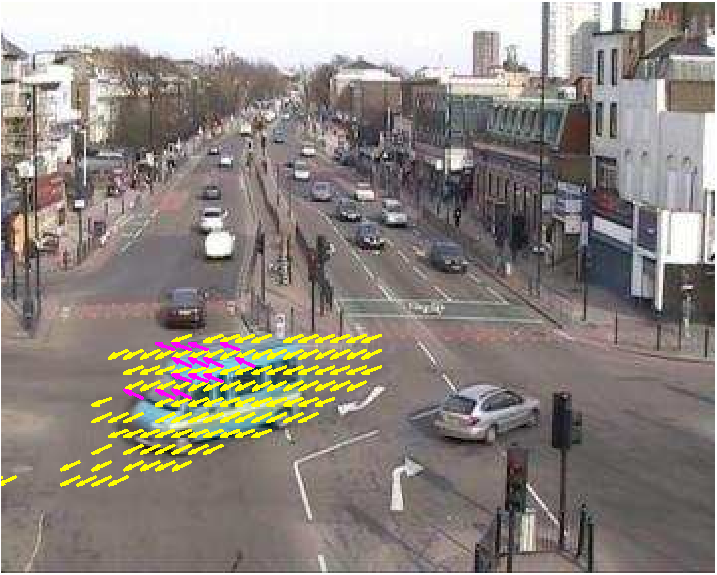
\includegraphics[width=3.7cm, height=2.5cm]{figures/qmul/t12-crop.pdf}}
	\subfigure[1.8\%]{
		\label{fig:subfigure:13}
		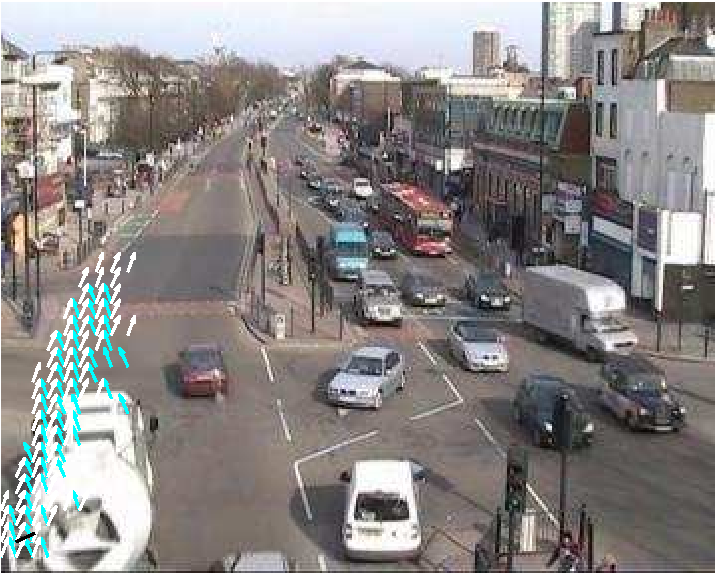
\includegraphics[width=3.7cm, height=2.5cm]{figures/qmul/t13-crop.pdf}}
	\subfigure[1.7\%]{
		\label{fig:subfigure:14}
		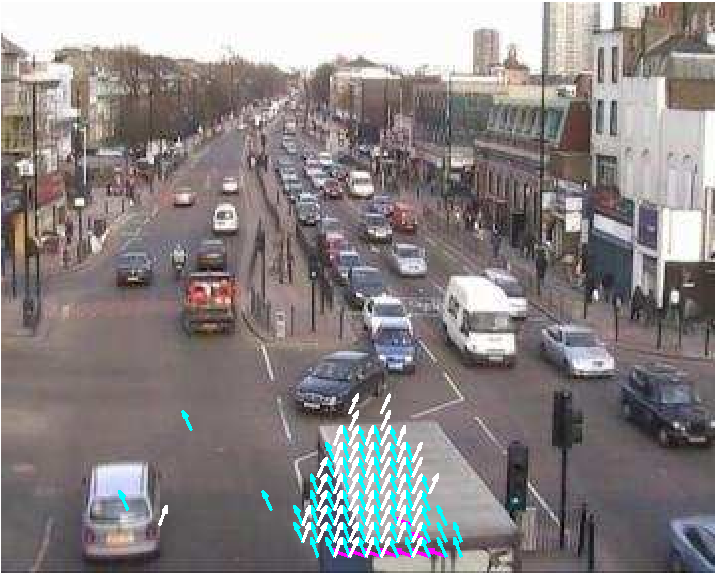
\includegraphics[width=3.7cm, height=2.5cm]{figures/qmul/t14-crop.pdf}}
	\subfigure[1.7\%]{
		\label{fig:subfigure:15}
		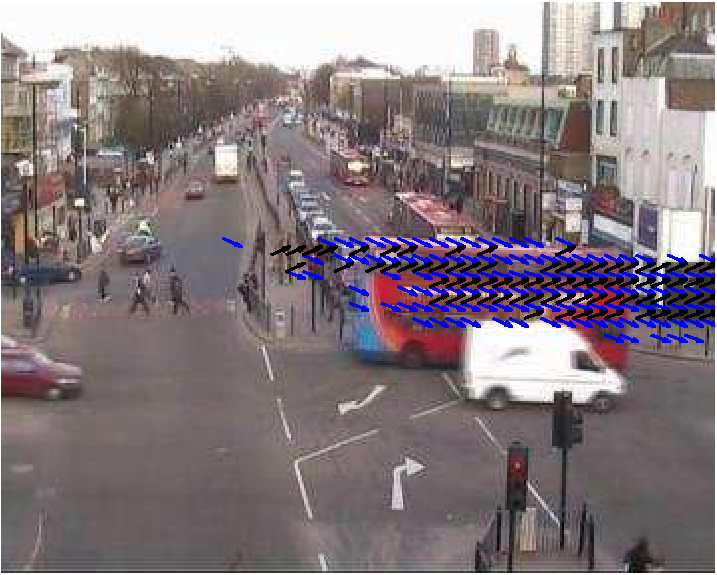
\includegraphics[width=3.7cm, height=2.5cm]{figures/qmul/t15-crop.pdf}}
	\subfigure[1.6\%]{
		\label{fig:subfigure:16}
		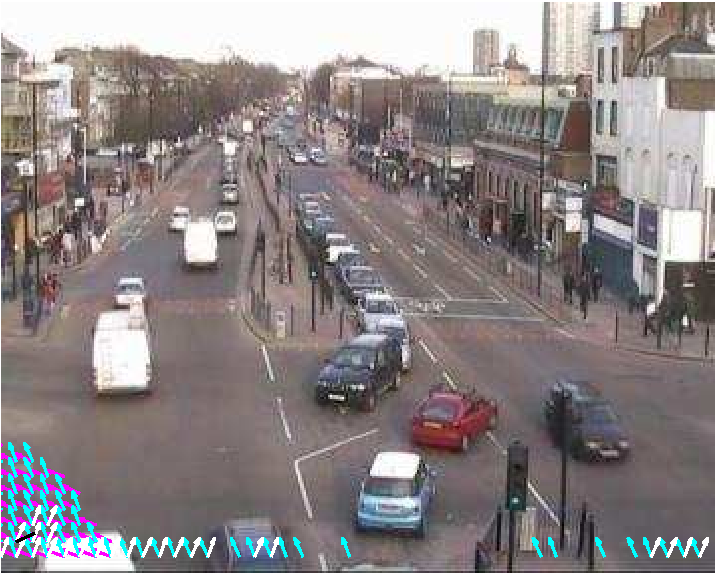
\includegraphics[width=3.7cm, height=2.5cm]{figures/qmul/t16-crop.pdf}}
	\subfigure[1.5\%]{
		\label{fig:subfigure:17}
		
		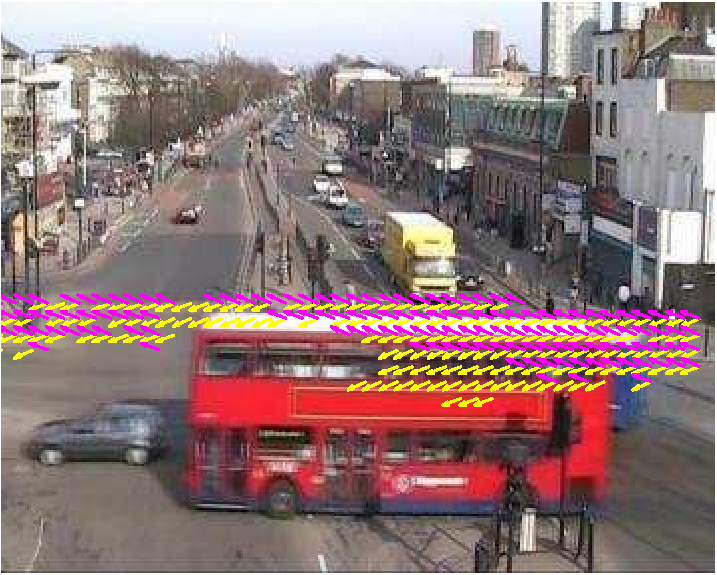
\includegraphics[width=3.7cm, height=2.5cm]{figures/qmul/t17-crop.pdf}}
	\subfigure[1.2\%]{
		\label{fig:subfigure:18}
		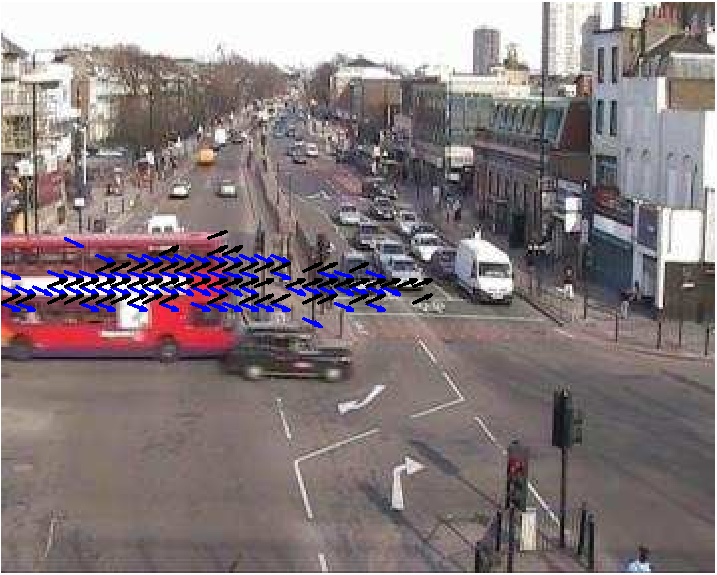
\includegraphics[width=3.7cm, height=2.5cm]{figures/qmul/t18-crop.pdf}}
	\subfigure[1\%]{
		\label{fig:subfigure:19}
		\includegraphics[width=3.7cm, height=2.5cm]{figures/qmul/t19-crop.pdf}}
	\subfigure[1\%]{
		\label{fig:subfigure:20}
		\includegraphics[width=3.7cm, height=2.5cm]{figures/qmul/t20-crop.pdf}}
	\subfigure[0.9\%]{
		\label{fig:subfigure:21}
		\includegraphics[width=3.7cm, height=2.5cm]{figures/qmul/t21-crop.pdf}}
	\subfigure[0.8\%]{
		\label{fig:subfigure:22}
		\includegraphics[width=3.7cm, height=2.5cm]{figures/qmul/t22-crop.pdf}}
	\subfigure[all possible lanes]{
		\label{fig:subfigure:qmul_path}
		\includegraphics[width=3.7cm, height=2.5cm]{figures/qmul/qmul_path-crop.pdf}}
	\subfigure[colors for directions]{
		\label{fig:directions}
		\includegraphics[width=3cm, height=3cm]{figures/8directions2-crop.pdf}}
	\caption[Typical activities in QMUL Junction Dataset]
	{(1)- (22) are typical activity patterns discovered by HDP models. The activities are sorted according to the number of the words assigned by the training corpus (in a descending order). (23) is the manually labeled legal vehicles driving lanes (red lines) and pedestrians walking lanes (yellow dash lines). The motion is quantified into eight directions and labeled in eight colors as (24).}
	\label{qmul_activity}
\end{figure}



\section{Dataset}
\label{dataset}
Three benchmark datasets were adopted in our experiment to evaluate our proposed method. Each of them is captured from a complicated crowded traffic junction, which is regulated by the traffic lights. Their details are listed as follows
\begin{itemize}
	\item[1]\textbf{QMUL Junction Dataset} \cite{hospedales2009markov}: This contains 1 hour of 25 fps video (90000 frames) with frame size $360\times288$. The video covers a busy traffic junction containing three major flows in different directions. 
	\item[2]\textbf{QMUL Junction Dataset 2} \cite{hospedales2009markov}: This video length is 52 minutes with 25 fps (78000 frames). The frame size is $360\times288$. This video is captured in a busy street with particularly busy pedestrian activity. 
	\item[3]\textbf{MIT Dataset}~\cite{wang2009unsupervised}: It consists of 1.5 hour of 30fps (162000 frames) with frame size $720\times 480$, and captures a far-field traffic scene.
\end{itemize}

\section{Parameter Setting}
\label{parameter}
To construct the codebook of visual words, we spatially divided the image scene into square cells of size $8\times8$. 
The local motions were quantified into eight directions as shown in~Fig.~\ref{fig:directions}. Therefore, the codebooks of both QMUL datasets have $12960$ words, while MIT contains $43200$ words. Each dataset was temporally segmented into non-overlapping video clips with $75$ frames. The threshold for optic flow estimation was 0.8.

For each dataset, the first 500 video clips (about 25 minute's length) were employed to learn the typical activities and traffic states. The rest of the video sequences were employed to simulate online screened video to test online performance, i.e., 699 clips of QMUL Junction Dataset, 539 clips of QMUL Junction Dataset 2 and 1711 clips of MIT Dataset were used for test.

The ARD kernel was adopted in both GP regression models and GP classification models. Their hyper-parameters were optimized by \emph{Conjugate Gradient} \cite{nocedal2006numerical}. The \emph{Laplace's } approximation method \cite{williams1998bayesian} was applied in GP classification models.

To infer the latent variables in HDP and HDP-HMM models, we exploited Gibbs sampling schemes for 1000 iterations. For the selection of their hyper-parameters $(\beta,\alpha)$, we performed a grid search on $\beta, \alpha\in \{0.1, 0.5, 1.0, 2.0\}$. 
We found that, even though the number of clusters increased with larger $\beta$ and $\alpha$, the numbers of typical activities and states always converged when at least $90\%$ of the total motions were explained. These numbers kept consistent when $\beta$ and $\alpha$ were both larger than 0.5. The additional clusters were generated to explain very rare motions. In this thesis, we were only interested in typical activities and states and we did not use topic models to estimate likelihood or posterior. Therefore, we did not need precise hyper-parameters. The hyper-parameters were fixed at $\beta = 2, \alpha=0.5$ for all experiments. In actual implementation of HDP and HDP-HMM models, the hyper-parameters can be optimized by giving a vague gamma prior and sampling them using the scheme proposed in~\cite{teh2006hdp}.


\section{Experiment on QMUL Junction Dataset}
\label{exp:qmul}
In this section, we will specially analyze the experimental process and results on QMUL Junction Dataset. The experimental results will be compared with others provided by some popular methods. Then, the experimental results on the other two datasets will be briefly illustrated and discussed.

\subsection{Learning Typical Activities and States}
\label{exp:qmul:activity_and_state}


The HDP models automatically learned 32 activities in this traffic scene, among which 22 were selected as typical activities, as shown in Fig.~\ref{qmul_activity}. Their corresponding percentages of how many words in the training corpus are assigned to them are noted. For a better illustration, we manually painted all possible motion flows for vehicles and pedestrians and marked them with alphabetic letters in~Fig.~\ref{fig:subfigure:qmul_path}. Each path is explained as follows:

\begin{figure}[!htbp]
	\renewcommand{\thesubfigure}{\arabic{subfigure}}
	%\renewcommand{\thefigure}{\arabic{figure}}
	\makeatletter
	\renewcommand{\@thesubfigure}{(\thesubfigure)\space}
	\renewcommand{\p@subfigure}{\thefigure.}
	\makeatother
	\centering
	\centering
	\subfigure[0.38\%]{
		\label{fig:subfigure:23}
		\includegraphics[width=3.7cm, height=2.5cm]{figures/qmul/t23-crop.pdf}}
	\subfigure[0.08\%]{
		\label{fig:subfigure:24}
		\includegraphics[width=3.7cm, height=2.5cm]{figures/qmul/t24-crop.pdf}}
	\subfigure[0.08\%]{
		\label{fig:subfigure:25}
		\includegraphics[width=3.7cm, height=2.5cm]{figures/qmul/t25-crop.pdf}}
	\subfigure[0.03\%]{
		\label{fig:subfigure:26}
		\includegraphics[width=3.7cm, height=2.5cm]{figures/qmul/t26-crop.pdf}}
	\subfigure[0.03\%]{
		\label{fig:subfigure:27}
		\includegraphics[width=3.7cm, height=2.5cm]{figures/qmul/t27-crop.pdf}}
	\subfigure[0.02\%]{
		\label{fig:subfigure:28}
		\includegraphics[width=3.7cm, height=2.5cm]{figures/qmul/t28-crop.pdf}}
	\subfigure[0.01\%]{
		\label{fig:subfigure:29}
		\includegraphics[width=3.7cm, height=2.5cm]{figures/qmul/t29-crop.pdf}}
	\subfigure[0.01\%]{
		\label{fig:subfigure:30}
		\includegraphics[width=3.7cm, height=2.5cm]{figures/qmul/t30-crop.pdf}}
	\caption[Rare activities in QMUL Junction Dataset]
	{8 rarely occurring activities.}
	\label{fig:rare_activity}
\end{figure} 


\begin{figure}[!htp]
	\subfigure[Vertical flow]{
		\begin{minipage}{0.45\linewidth}
			\centering\includegraphics[width = 4cm]{figures/qmul/ss1-crop.pdf}\\
			\vfill
			\centering\includegraphics[width = 5.2cm]{figures/qmul/hist_s1-crop.pdf}
		\end{minipage}
		\label{fig:subfigure:state1}
	}
	\hfill
	\subfigure[Leftward flow]{
		\begin{minipage}{0.45\linewidth}
			\centering\includegraphics[width = 4cm]{figures/qmul/ss3-crop.pdf}\\
			\vfill
			\centering\includegraphics[width = 5.2cm]{figures/qmul/hist_s3-crop.pdf}
		\end{minipage}
		\label{fig:subfigure:state2}
	}
	\hfill
	\subfigure[Rightward flow]{
		\begin{minipage}{0.45\linewidth}
			\centering\includegraphics[width = 4cm]{figures/qmul/ss2-crop.pdf}\\
			\vfill
			\centering\includegraphics[width = 5.2cm]{figures/qmul/hist_s2-crop.pdf}
		\end{minipage}
		\label{fig:subfigure:state3}
	}
	\hfill
	\subfigure[Left and right turn]{
		\begin{minipage}{0.45\linewidth}
			\centering\includegraphics[width = 4cm]{figures/qmul/ss4-crop.pdf}\\
			\vfill
			\centering\includegraphics[width = 5.2cm]{figures/qmul/hist_s4-crop.pdf}
		\end{minipage}
		\label{fig:subfigure:state4}
	}		
	\caption[Typical traffic states in QMUL Junction Dataset]{4 typical traffic states are learned by HDP-HMM model. The states are sorted according to the traffic light cycle. Their corresponding average mixtures of typical activities throughout the training set are shown in the histograms. The x-axis is the index of atomic activities and the y-axis is the percentage of each atomic activity.}
	\label{qmul_state}
\end{figure}

\begin{itemize}
	\item Flow a: Vehicles driving upward from bottom in the left traffic lane. Topic 2, 5, 13 and 21 form this flow.
	\item Flow b: Vehicles driving downward from top in the left traffic lane. It is mainly explained by topics 1, 8 and 20. Part of topic 10 also covers this flow.
	\item Flow c: Vehicles from top turning left. It can be explained by topics 6 and 20.
	\item Flow d: Vehicles turning left from the left entrance. It is explained by the upper part of topic 4.
	\item Flow e: Vehicles in the left bottom corner turning left, as shown in topic 16.
	\item Flow f: Vehicles from top making a right turn in the middle of the junction, as shown in topics 12 and 7.
	\item Flow g: Vehicles from bottom making a right turn in the middle of the junction. Topic 14 is its first step: vehicles driving into the middle area from bottom and waiting for time to make a right turn as topic 9.
	\item Flow h (leftward) and i: Vehicles driving leftward and part of them making a right turn. It is dominated by topic 3, 7 and 19. Topic 17 also explains such flow caused by high vehicles such as double-decker buses.
	\item Flow h (rightward) and j: Vehicles driving rightward and part of them making a right turn. It mainly consists of topics 4, 6 and 10. Topics 15 and 18 also explain such flow caused by high vehicles.
	\item Flow k and l: Pedestrian crossing the road in topics 15 and 18 rightward and in topic 17 leftward.
	\item Flow m: People crossing the road in the right bottom corner. %\subsection{Abnormality Detection}
\end{itemize}



Fig.~\ref{fig:rare_activity} shows the 8 rarely occurring activities learned by the HDP models. From the figure we can see, some of them are caused by rarely occurring abnormal events: in Fig.~\ref{fig:subfigure:24} the people is walking in the area for vehicles (middle bottom); Fig.~\ref{fig:subfigure:28} is caused by a police car diving reversely ; Fig.~\ref{fig:subfigure:26} shows something crossing the left lane where for vehicles driving upward. Motions distribute in the other rare activity patterns in chaos. They are caused by noise or lighting changing.

The HDP-HMM models automatically learned 9 traffic states. We selected 4 of them as typical states, which have the highest percentage among all clips, as shown in Fig.~\ref{qmul2_state}. Their corresponding average feature vectors over the training set are shown below them. Each state is explained as follows:
\begin{itemize}
	\item Vertical flow: Topics 1 and 2 dominate in this interaction. The other topics such as 5, 8 and 10 related to vertical traffic topics have also relative high values in the histogram.
	\item Leftward flow: It mainly consists by topics 4, 6 and 10. Topics 1, 8 and 9 overlap this flow. The feature values of topics 15 and 18 are relative high because of pedestrians.
	\item Rightward flow: It is absolutely dominated by topic 3. Topics 7, 12, 17 and 19 are also important components. The feature values of topics 11, 17 and 22 are relative high because of pedestrians.
	\item Left and right turn: This state happens during the state of vertical flow, when the vertical flow temporally terminates. It is a complicated interaction among a couple of topics, such as topics 1, 3, 6, 7, 8 and 12.
\end{itemize}

\begin{figure}[!htbp]
	\centering
	\includegraphics[width=5cm]{figures/transition_qmul-crop.pdf}
	\caption[State transition graph of QMUL Junction Dataset]{State transition graph for QMUL Junction Dataset. The arrow indicates the transition direction and the number denote the transition probability.}
	\label{fig:qmul_transition}
\end{figure}

Fig.\ref{fig:qmul_transition} illustrates the state transition directions (arrows) and the corresponding transition probabilities. From the graph we can see, the transition is in a strict order. However, there is still a very low probability for the transition from state A to C (0.02), C to B (0.05) and B to D (0.05). It might be caused by emergency vehicles cutting off current state and changing it, or some training video clips being falsely clustered by HDP-HMM models.


\subsection{Online Classifying Traffic States}
\label{exp:qmul:online classify} 
We used the rest part of the video sequence (699 clips) to simulate the online classification task.
Each 75 newly screened video frames were segmented into a clip.
%The online screened video stream was segmented into clips of 75 frames each. 
Then the high-level features were extracted to represent the state in this clip. 
Using our classifier it was assigned with one of the four state labels.
Fig.~\ref{fig:online_exsample_qmul} shows an example for each traffic state that was recognized in 4 clips from online capture video sequence, respectively. Their corresponding high-level features $\mathbf{c}_t =\{p_{t1},\cdots,p_{tK}\}$ are illustrated below. For comparison, the mean features' value of each state are marked by the red curves.
To lively illustrate the construction of an interaction during a clip, the interaction in Fig.~\ref{fig:s4_exsample} is decomposed into 5 main typical activities, as shown in Fig.~\ref{fig:qmul:interaction_decomposition}. 

We have manually labeled each clip to validate the classification results by our model. The confusion matrix is shown in Tab.~\ref{tab:qmul_confuse}. From the matrix we see that, our model have a very high classification accuracy. 4 clips are falsely classified as shown in Fig.~\ref{fig:qmul_falsely_classified}. Even with the help of transition information these wrong results can be modified. Fig.~\ref{fig:qmul_classification_result} shows the labels of the 699 test video clips. Note the periodicity of the labels assigned. We can observe that each traffic cycle lasts around 40 clips i.e. 120 seconds.
We have also compared our classification results with those generated by popular methods in Tab.~\ref{tab:qmul_compare}. From the table we see that our model outperforms other three popular methods in terms of classification results. 
Notice that, this comparison is for your information only. 
Normally, the learned traffic states are different by using different methods. Our method has learned the same traffic states in this dataset as others by chances, because the main traffic state in this scene are very explicit. On the other side, different studies often adopt different length of video clips, such as ours is 75 frames each clip while in~\cite{hospedales2009markov} was 25 frames and in~\cite{wang2009unsupervised} was 300 frames. It might leads to different results. We have not implemented others methods to achieve results under the same conditions of our experiments.
Therefore, for objective comparison and evaluation, we will not compare our method with the others in the other two datasets any more.
\begin{table}[!htbp]
	\begin{center}
		\renewcommand\arraystretch{2}
		\setlength{\tabcolsep}{8pt}
		\begin{tabular}{c c|c|c|c|c|}
			\multicolumn{1}{c}{ }	& \multicolumn{5}{c}{Our Classification }\\
			\multirow{5}{5pt}{\rotatebox{90}{Manually label}}		&\multicolumn{1}{c}{ }	&\multicolumn{1}{c}{a}	&\multicolumn{1}{c}{b}	&\multicolumn{1}{c}{c}	&\multicolumn{1}{c}{d}\\
			\cline{3-6}
			&a		&367	&0	&0	&0\\
			\cline{3-6}
			&b		&0	&143	&0	&1\\
			\cline{3-6}
			&c		&0	&0	&120	&0\\
			\cline{3-6}
			&d		&3	&0		&0	&64\\
			\cline{3-6}
		\end{tabular}
	\end{center}
	\caption[The confusion matrix of QMUL Juction Dataset]
	{The confusion matrix of QMUL Juction Dataset}
	\label{tab:qmul_confuse} 
\end{table}


We want to point it out that more clips would be falsely classified if only using the GP classifier. Fig.~\ref{fig:qmul_revised_detect} shows an example that the clip 667 was classified into state D but its previous clip was in state B and its following clip was state C. Hence, clip 667 should be the end of state B. According to the state transition graph (see Fig.~\ref{fig:qmul_transition}), transition probability from state B to state C is only 0.05. Hence, the classification result was corrected as state B by our model.

\begin{landscape}
	\begin{table}[!htbp]
		\begin{center}
			\renewcommand\arraystretch{1.5}
			\setlength{\tabcolsep}{7pt}
			\begin{tabular}{l | c c c c | c c c c | c c c c | c c c c}
				\toprule[1pt] 
				\multirow{2}{*}{State}		&\multicolumn{4}{c|}{MCTM}	&\multicolumn{4}{c|}{LDA}	&\multicolumn{4}{c|}{HMM}		&\multicolumn{4}{c}{Ours}\\
				\cmidrule{2-5}		\cmidrule{6-9}		\cmidrule{10-13}	\cmidrule{14-17}
				&L	&R	&V	&VT	&L	&R	&V	&VT	&L	&R	&V	&VT	&L	&R	&V	&VT\\
				\midrule[1pt]
				Left	&\textbf{.99}	&.00	&.00	&.01	&\textbf{.49}	&.44	&.00	&.06	&\textbf{.98}	&.00	&.01	&.01	
				
				&\textbf{1.0}	&.00	&.00	&.00\\
				
				Right	&.00	&\textbf{.94}	&.01	&.05	&.00	&\textbf{1.0}	&.00	&.00	&.00	&\textbf{.92}	&.08	&.00	
				
				&.00	&\textbf{.99}	&.00	&.01\\
				
				Vertical	&.00	&.00	&\textbf{.77}	&.22	&.01	&.17	&\textbf{.82}	&.00	&.02	&.01	&\textbf{.69}	&.28	
				
				&.00	&.00	&\textbf{1.0}	&.00\\
				
				Vertical-Turn	&.31	&.05	&.20	&\textbf{.43}	&.01	&.21	&.30	&\textbf{.46}	&.49	&.04	&.32	&\textbf{.15}	
				
				&.05	&.00	&.00	&\textbf{.95}\\
				\cmidrule{1-17}	
				Average Accuracy		&\textbf{.78}	&	&	&	&\textbf{.69}	&	&	&	&\textbf{.69}	&	&	&	
				
				&\textbf{.99}	&	&	&\\	%[5ex]
				
				\bottomrule[1pt] 
				
			\end{tabular}
		\end{center}
		\caption[Comparison of Classification results between our methods and others popular methods for QMUL Juction Dataset]
		{Comparison of Classification results between our methods and others popular methods for QMUL Juction Dataset: The results of MCTM, LDA and HMM are cited from ~\cite{hospedales2012video}}
		\label{tab:qmul_compare} 
	\end{table}
\end{landscape}



\clearpage
\newpage
\begin{figure}[!htbp]
	\subfigure[Vertical flow]{
		\begin{minipage}{0.45\linewidth}
			\centering\includegraphics[width = 5cm]{figures/qmul/s3_example_686-crop.pdf}\\
			\vspace{0.3cm}
			\centering\includegraphics[width = 6.5cm]{figures/qmul/s3_example_hist_686-crop.pdf}
		\end{minipage}
		\label{fig:s3_exsample}
	}
	\hfill
	\subfigure[Leftward flow]{
		\begin{minipage}{0.45\linewidth}
			\centering\includegraphics[width = 5cm]{figures/qmul/s4_example_699-crop.pdf}\\
			\vspace{0.3cm}
			\centering\includegraphics[width = 6.5cm]{figures/qmul/s4_example_hist_699-crop.pdf}
		\end{minipage}
		\label{fig:s4_exsample}
	}
	\hfill
	\subfigure[Rightward flow]{
		\begin{minipage}{0.45\linewidth}
			\centering\includegraphics[width = 5cm]{figures/qmul/s1_example_708-crop.pdf}\\
			\vspace{0.3cm}
			\centering\includegraphics[width = 6.5cm]{figures/qmul/s1_example_hist_708-crop.pdf}
		\end{minipage}
		\label{fig:s1_exsample}
	}
	\hfill
	\subfigure[Left and right turn]{
		\begin{minipage}{0.45\linewidth}
			\centering\includegraphics[width = 5cm]{figures/qmul/s8_example_832-crop.pdf}\\
			\vspace{0.3cm}
			\centering\includegraphics[width = 6.5cm]{figures/qmul/s8_example_hist_832-crop.pdf}
		\end{minipage}
		\label{fig:s8_exsample}
	}
	\caption[Examples of online classification in QMUL Junction Dataset]
	{We show a video clip as an example for each type of traffic state in the first row. Their corresponding features histograms are shown in the second row. For comparison, the red curve in each plot is the average activity mixture over the training video.}
	\label{fig:online_exsample_qmul}
\end{figure}

\clearpage
\newpage
\begin{landscape}
	\begin{figure}[!htbp]
		\centering
		\includegraphics[width = 20cm]{figures/qmul/construct_example_699_new.pdf}
		\caption[Decomposition of an interaction into main activities]
		{The interaction in the video clip Fig.~\ref{fig:s4_exsample} is decomposed into five main activities.}
		\label{fig:qmul:interaction_decomposition}
	\end{figure}
\end{landscape}

\begin{figure}[!htbp]
	\centering
	\subfigure[]{
		\includegraphics[width = 5.5cm]{figures/qmul/falsedetect/542_s3s8-crop.pdf}
	}\hspace{1cm}
	\subfigure[]{
		\includegraphics[width = 5.5cm]{figures/qmul/falsedetect/543_s3s8-crop.pdf}
	}
	\subfigure[]{
		\includegraphics[width = 5.5cm]{figures/qmul/falsedetect/617_s3s8-crop.pdf}
	}\hspace{1cm}
	\subfigure[]{
		\includegraphics[width = 5.5cm]{figures/qmul/falsedetect/1043_s8s4-crop.pdf}
	}
	\caption[Falsely classified clips in QMUL Junction Dataset]{The four falsely classified clips in QMUL Junction Dataset.}
	\label{fig:qmul_falsely_classified}
\end{figure}

\begin{figure}[!htbp]
	\centering
	\subfigure[clip 666]{
		\includegraphics[width = 4cm]{figures/qmul/falsedetect/666_s4-crop.pdf}
	}
	\subfigure[clip 667]{
		\includegraphics[width = 4cm]{figures/qmul/falsedetect/667_s8s4-crop.pdf}
	}
	\subfigure[clip 668]{
		\includegraphics[width = 4cm]{figures/qmul/falsedetect/668_s1-crop.pdf}
	}
	\caption[Transition information corrected the falsely classified result by GP model]{An example for falsely classified result by GP model being corrected by using transition information.}
	\label{fig:qmul_revised_detect}
\end{figure}

\clearpage
\newpage
\begin{landscape}
	\begin{figure}[h]
		\centering
		\subfigure[ The classification results of 699 video clips]{
			\includegraphics[width = 22cm]{figures/qmul/qmul_state_sequence.png}
		}\\
		\subfigure[Zoom in of the classification result rom clip 400 to clip 520]{
			\includegraphics[width = 22cm]{figures/qmul/qmul_state_sequence_zoom.png}
		}
		\caption[Classification results of QMUL Junction Dataset]{Classification results of 699 video clips. In both histograms the x-axis is the index of video clips in temporal order and the y-axis is the label of the four traffic states shown in Fig.~\ref{qmul_state}}
		\label{fig:qmul_classification_result}
	\end{figure}
\end{landscape}


%%*****************************************************************************
%%=============================================================================
\clearpage
\newpage
\subsection{Abnormal Events Detection}
\label{exp:qmul:online classify} 
The three kinds of abnormal events were identified as discussed in Sec.~\ref{framework:abnormal}, respectively. In this QMUL Junction scene the main abnormal events include Jaywalking, illegal U-turn and emergencies caused by ambulances, fire engines and police cars. Some of the examples for each kind of abnormal event are illustrated as following. Fig.~\ref{fig:rare_motion_abnormalevents} illustrates the two abnormal events caused by rarely occurring motions. For example, the motions of the ambulance have never occurred in the training data Fig.~\ref{fig:qmul_ambulance}. The ambulance is driving in an absolutely forbidden direction in the lane.

\begin{figure}[!htbp]
	\centering
	\subfigure[Ambulance]{
		\includegraphics[width = 6cm, height=4.5cm]{figures/qmul/abnormal/ambulance_212.png}
		\label{fig:qmul_ambulance}
	}
	\hspace{1.5cm}
	\subfigure[Pedestrian walking in improper area]{
		\includegraphics[width = 6cm, height=4.5cm]{figures/qmul/abnormal/jw3_354.png}
		\label{fig:qmul_jaywalking1}
	}
	\caption[Abnormal Events caused by rarely occurring motions]{Abnormal Events caused by rarely occurring motions. In the training dataset such motions have rarely or never occurred. They do not belong to any typical activities. The red boxes highlight the abnormal agents.}
	\label{fig:rare_motion_abnormalevents}
\end{figure}

In Fig.~\ref{fig:illegal_transition}, the traffic state is forced to change in an illegal ordering due to the fire engine. 
The rightward flow should not follow the vertical flow according to the learning results by HDP-HMM models. Therefore, the  clip was identified as abnormal event, even though its appearance is definitely a right flow state.

\begin{figure}[!htbp]
	\centering
	\begin{minipage}{0.26\textwidth}
		\includegraphics[width=5cm]{figures/qmul/fireengine_412-crop.pdf}\\
		\centering\scriptsize{Vertical flow in $t-1$ clip}
	\end{minipage}
	\hspace{1cm}
	%\caption{Vertical flow in $t-1$ clip}
	\begin{minipage}{0.26\textwidth}
		\includegraphics[width=5cm]{figures/qmul/abnormal/fireengine_413.png}
		\centering\scriptsize{Fire engine presents in $t$ clip}
	\end{minipage}
	\hspace{1cm}
	%\caption{Fire engine present in $t$ clip}
	\begin{minipage}{0.26\textwidth}
		\includegraphics[width=5cm]{figures/qmul/abnormal/fireengine_414.png}
		\centering\scriptsize{Rightward flow in $t+1$ clip}
	\end{minipage}
	\caption[Abnormal Event caused by illegal state transition]{Abnormal Event caused by illegal state transition. A fire engine interrupts the current vertical flow. The red boxes highlight the abnormal agents. }
	\label{fig:illegal_transition}
\end{figure}

Normally, abnormal events are caused by conflicting activities like Jaywalking, illegal U-turn converse driving or aggressively cutting in other roads. 
We illustrate an example for each type of such conflicting activities in Fig~.\ref{fig:qmul:conflict_activities}. 
The conflicting activities were detected by our GP regression models as discussed in Sec.~\ref{framework:abnormal}. If the observed value (blue bar) of any activities is larger than its predicted value (green curve and circle) as $1.96\sigma$ (red curve and cross), it is judged as a conflict activity against the others. The abnormally acting agents are marked by red boxes. 
They are analyzed in detail as following (all the related atomic activities are founded in Fig.~\ref{qmul_activity}):
\begin{itemize}
	\item Fig.~\ref{fig:qmul_police1} and ~\ref{fig:qmul_police2} show the police car driving conversely.
	\item This counter flow induces the value of activities 3 and 17 in the former clip, activities 3 and 19 in the latter clip. 
	\item A fire engine cuts off the vertical flow (see Fig.~\ref{fig:qmul_fireengine1}) and causes the activity 4 much stronger than the prediction.
	\item In Fig.~\ref{fig:qmul_uturn} the activity 19 is abnormal because of a vehicle making an illegal U-turn. 
\end{itemize}

Fig.~\ref{fig:qmul_missdetec_abnorml} shows some missing detected abnormal events. Because our method is beyond detecting, the categories of activity agents are not considered. For example, if a pedestrian is walking along the path of vehicles, it will not be detected as an abnormality, as shown in Fig.~\ref{fig:qmul_missdetect_bike} and~\ref{fig:qmul_missdetect_people}. 
In Fig.~\ref{fig:qmul_missdetect_fireengine}, before the fire engine drives into the camera scene, all vehicles have stopped and wait for its pass. Therefore, there is no activity in conflict with the fire engine. The scene is classified as leftward state. Because of its previous state is the sate left and right turn, this transition is legal. That is why this emergency was undetected.
A car is making an illegal U-turn in Fig.~\ref{fig:qmul_missdetect_uturn}. However, its activity seems identical with others in the leftward state. Hence, it is also not identified as an abnormal activity. The detection and tracking based approaches would perform better in this case.

\begin{figure}[!htbp]
	\centering\
	\subfigure[]{
		\includegraphics[width = 4.7cm]{figures/qmul/abnormal/false_detect_805-crop.pdf}
		\label{fig:qmul_flase_detect1}
	}
	\subfigure[]{
		\includegraphics[width = 4.7cm]{figures/qmul/abnormal/false_detect_881-crop.pdf}
		\label{fig:qmul_flase_detect1}
	}
	\subfigure[]{
		\includegraphics[width = 4.7cm]{figures/qmul/abnormal/false_detect_920-crop.pdf}
		\label{fig:qmul_flase_detect1}
	}
	\caption[Falsely detected Abnormal events by the GP regression models]{Falsely detected Abnormal events by the GP regression models}
	\label{fig:qmul_false_detected}
\end{figure}

Some falsely detected abnormalities are shown in Fig.~\ref{fig:qmul_false_detected}. The red double-decker bus is detected as a U-turn agent due to its big size. In Fig.~\ref{fig:qmul_flase_detect1}, a conflict activity is detected occurring in the right bottom of the camera scene, because in this state, there should not be a leftward traffic flow. However, this alarm is a misunderstanding by our models because of the bad video clip segmentation. This clip contains the state transition and is classified as the left and right turn state. 
Therefore, the GP regression models thought the activity conflicting with others in this state and judged it as an abnormal event. 
Actually, this activity occurred when the state has already changed into the state of leftward flow.

\begin{figure}[!htbp]
	\centering
	\subfigure[Bicycle in improper region]{
		\includegraphics[width = 6cm, height=4.5cm ]{figures/qmul/abnormal/bike_1004.png}
		\label{fig:qmul_missdetect_bike}
	}
	\hspace{1.5cm}
	\subfigure[People in improper region]{
		\includegraphics[width = 6cm, height=4.5cm]{figures/qmul/abnormal/underected_jw_88.png}
		\label{fig:qmul_missdetect_people}
	}
	\subfigure[Emergency cased by yire engine]{
		\includegraphics[width = 6cm, height=4.5cm]{figures/qmul/abnormal/fire_508.png}
		\hspace{1.5cm}
		\includegraphics[width = 6cm, height=4.5cm]{figures/qmul/abnormal/fire_509.png}
		\label{fig:qmul_missdetect_fireengine}
	}
	\subfigure[Illegal U-turn]{
		\includegraphics[width = 6cm, height=4.5cm]{figures/qmul/abnormal/undetect_uturn_1001.png}
		\hspace{1.5cm}
		\includegraphics[width = 6cm, height=4.5cm]{figures/qmul/abnormal/undetect_uturn_1002.png}
		\label{fig:qmul_missdetect_uturn}
	}
	\caption[Examples of missing detected abnormal events]{Examples of missing detected abnormal events}
	\label{fig:qmul_missdetec_abnorml}
\end{figure}




\begin{figure}[!htbp]
	\subfigure[Police car driving conversely 1]{
		\begin{minipage}{0.45\linewidth}
			\centering\includegraphics[width = 3.7cm]{figures/qmul/abnormal/police_892.jpg}\\
			\vfill
			\centering\includegraphics[width = 5.2cm]{figures/qmul/abnormal/police_892_hist-crop.pdf}
		\end{minipage}
		\label{fig:qmul_police1}
	}
	\hfill
	\subfigure[Police car driving conversely 2]{
		\begin{minipage}{0.45\linewidth}
			\centering\includegraphics[width = 3.7cm]{figures/qmul/abnormal/police_893.jpg}\\
			\vfill
			\centering\includegraphics[width = 5.5cm]{figures/qmul/abnormal/police_893_hist-crop.pdf}
		\end{minipage}
		\label{fig:qmul_police2}
	}
	\hfill
	\subfigure[Fire engine cuts off the flow]{
		\begin{minipage}{0.45\linewidth}
			\centering\includegraphics[width = 3.7cm]{figures/qmul/abnormal/fireengine_413.png}\\
			\vfill
			\centering\includegraphics[width = 5.5cm]{figures/qmul/abnormal/fireengine_413_hist-crop.pdf}
			\label{fig:qmul_fireengine1}
		\end{minipage}
	}
	\hfill
	\subfigure[Illegal U-turn]{
		\begin{minipage}{0.45\linewidth}
			\centering\includegraphics[width = 3.7cm]{figures/qmul/abnormal/uturn_423.png}\\
			\vfill
			\centering\includegraphics[width = 5.5cm]{figures/qmul/abnormal/uturn_423_hist-crop.pdf}
			\label{fig:qmul_uturn}
		\end{minipage}
	}
	\hfill
	\subfigure[Jaywalking]{
		\begin{minipage}{0.45\linewidth}
			\centering\includegraphics[width = 3.7cm]{figures/qmul/abnormal/jw_1141.png}\\
			\vfill
			\centering\includegraphics[width = 5.5cm]{figures/qmul/abnormal/jw_1141_hist-crop.pdf}
			\label{fig:qmul_uturn}
		\end{minipage}
	}
	\hfill
	\subfigure[Near collision]{
		\begin{minipage}{0.45\linewidth}
			\centering\includegraphics[width = 3.7cm]{figures/qmul/abnormal/near_collision_882.png}\\
			\vfill
			\centering\includegraphics[width = 5.5cm]{figures/qmul/abnormal/near_collision_882_hist-crop.pdf}
			\label{fig:qmul_uturn}
		\end{minipage}
	}
	\caption[Abnormal Events caused by conflicting activities]{Examples of typical abnormal events caused by conflicting activities. The observed values of each activity are represented by blue bars. The green curves (circles) note the predicted values $m$ and the red curves (crosses) equal $m+1.96\sigma$, i.e. the upper bounds of $95\%$ confidence region.}
	\label{fig:qmul:conflict_activities}
\end{figure}

We provide a human interpreted summary of the categories of abnormal events (in the test dataset) in Tab.~\ref{tab:qmul_discovered_abnormal}. Notice that, each entire abnormal event is counted as one event, no matter how many clips it spans. The false detection means that, a clip is detected as an abnormal clip, but there is not any abnormal event of interest. The overall false positive rates is defined as:
\begin{equation*}
	FPR = \frac{\mbox{Number of falsely detected clips}}{\mbox{Number of test clips}}.
\end{equation*}
\begin{table}[!htbp]
	\begin{center}
		\renewcommand\arraystretch{1.8}
		\setlength{\tabcolsep}{5pt}
		\begin{tabular}{|c| c|c|}
			\hline
			Types			& Detected		& Total\\
			\hline
			Jaywalking		& 11			& 19\\
			Emergency		& 3				& 4\\
			Illegal U-turn  & 7				& 10\\
			Near collision  & 2				& 2\\ 
			Strange driving & 2				& 1\\
			Improper region & 0				& 2\\
			False detect    & 18            & $\setminus$\\
			\hline
			Overall TPR     &$66\%$			&\\
			Overall FPR     &$2.6\%$		&\\
			\hline
		\end{tabular}
	\end{center}
	\caption[Summary of discovered abnormal events QMUL Juction Dataset]
	{Summary of discovered abnormal events of QMUL Juction Dataset. Overall true positive and false positive rates are also given.}
	\label{tab:qmul_discovered_abnormal} 
\end{table}

%%*****************************************************************************
%%=============================================================================
\clearpage
\newpage
\section{Experiment on QMUL Junction Datasets 2}
\label{exp:qmul2} 
The HDP models automatically learned 45 activities in QMUL Junction 2 Dataset, among which 21 were selected as typical activities, as shown in Fig.~\ref{qmul2_activity}. Their corresponding percentages of how many words in the training corpus are assigned to them are noted. For a better illustration, we manually painted all possible motion flows for vehicle and pedestrians and marked them with alphabetic letters in~Fig.~\ref{fig:qmul2_path}. Each path is explained as follows.

\begin{itemize}
	\item Flow a: Vehicles driving downward from top in the right traffic lane. Activities 4, 13 and 17 form this flow.
	\item Flow b: Vehicles driving upward from bottom in the left traffic lane. Activities 2, 5, 9 and 20 form this flow.
	\item Flow c: Vehicles from top in the right traffic lane making a right turn in the middle of the junction, as shown in activities 1, 6, 16 and 21.
	\item Flow d: Vehicles turning left from the left entrance. It is explained by the upper part of activities 7 and 19.
	\item Flow e: Pedestrian crossing the right traffic lane leftward in activities 12, 15 and 18.
	\item Flow f: Pedestrian crossing the left traffic lane leftward in activities 8 and 10.
	\item Flow g: Pedestrian crossing the left traffic lane rightward in activity 3.
	\item Flow h: Pedestrian crossing the right traffic lane rightward in activities 11 and 14.
\end{itemize}

\begin{figure}[!htbp]
	\renewcommand{\thesubfigure}{\arabic{subfigure}}
	%\renewcommand{\thefigure}{\arabic{figure}}
	\makeatletter
	\renewcommand{\@thesubfigure}{(\thesubfigure)\space}
	\renewcommand{\p@subfigure}{\thefigure.}
	\makeatother
	\centering
	\subfigure[17.2\%]{
		\label{fig:qmul2:1}
		\includegraphics[width=3.7cm, height=2.5cm]{figures/qmul_2/t1-crop.pdf}}
	\subfigure[14.1\%]{
		\label{fig:qmul2:2}
		\includegraphics[width=3.7cm, height=2.5cm]{figures/qmul_2/t2-crop.pdf}}
	\subfigure[6.5\%]{
		\label{fig:qmul2:3}
		\includegraphics[width=3.7cm, height=2.5cm]{figures/qmul_2/t3-crop.pdf}}
	\subfigure[6.1\%]{
		\label{fig:qmul2:4}
		\includegraphics[width=3.7cm, height=2.5cm]{figures/qmul_2/t4-crop.pdf}}
	\subfigure[5.2\%]{
		\label{fig:qmul2:5}
		\includegraphics[width=3.7cm, height=2.5cm]{figures/qmul_2/t5-crop.pdf}}
	\subfigure[5.1\%]{
		\label{fig:qmul2:6}
		\includegraphics[width=3.7cm, height=2.5cm]{figures/qmul_2/t6-crop.pdf}}
	\subfigure[4.7\%]{
		\label{fig:qmul2:7}
		\includegraphics[width=3.7cm, height=2.5cm]{figures/qmul_2/t7-crop.pdf}}
	\subfigure[4.5\%]{
		\label{fig:qmul2:8}
		\includegraphics[width=3.7cm, height=2.5cm]{figures/qmul_2/t8-crop.pdf}}
	\subfigure[4.5\%]{
		\label{fig:qmul2:9}
		\includegraphics[width=3.7cm, height=2.5cm]{figures/qmul_2/t9-crop.pdf}}
	\subfigure[4.1\%]{
		\label{fig:qmul2:10}
		\includegraphics[width=3.7cm, height=2.5cm]{figures/qmul_2/t10-crop.pdf}}
	\subfigure[3.9\%]{
		\label{fig:qmul2:11}
		\includegraphics[width=3.7cm, height=2.5cm]{figures/qmul_2/t11-crop.pdf}}
	\subfigure[3.5\%]{
		\label{fig:qmul2:12}
		\includegraphics[width=3.7cm, height=2.5cm]{figures/qmul_2/t12-crop.pdf}}
	\subfigure[3.4\%]{
		\label{fig:qmul2:13}
		\includegraphics[width=3.7cm, height=2.5cm]{figures/qmul_2/t13-crop.pdf}}
	\subfigure[2.8\%]{
		\label{fig:qmul2:14}
		\includegraphics[width=3.7cm, height=2.5cm]{figures/qmul_2/t14-crop.pdf}}
	\subfigure[2.6\%]{
		\label{fig:qmul2:15}
		\includegraphics[width=3.7cm, height=2.5cm]{figures/qmul_2/t15-crop.pdf}}
	\subfigure[2.4\%]{
		\label{fig:qmul2:16}
		\includegraphics[width=3.7cm, height=2.5cm]{figures/qmul_2/t16-crop.pdf}}
	\subfigure[2.2\%]{
		\label{fig:qmul2:17}
		\includegraphics[width=3.7cm, height=2.5cm]{figures/qmul_2/t17-crop.pdf}}
	\subfigure[1.7\%]{
		\label{fig:qmul2:18}
		\includegraphics[width=3.7cm, height=2.5cm]{figures/qmul_2/t18-crop.pdf}}
	\subfigure[1.0\%]{
		\label{fig:qmul2:19}
		\includegraphics[width=3.7cm, height=2.5cm]{figures/qmul_2/t19-crop.pdf}}
	\subfigure[1.0\%]{
		\label{fig:qmul2:20}
		\includegraphics[width=3.7cm, height=2.5cm]{figures/qmul_2/t20-crop.pdf}}
	\subfigure[0.6\%]{
		\label{fig:qmul2:21}
		\includegraphics[width=3.7cm, height=2.5cm]{figures/qmul_2/t21-crop.pdf}}
	\subfigure[all possible lanes]{
		\label{fig:qmul2_path}
		\includegraphics[width=3.7cm, height=2.5cm]{figures/qmul_2/junction_path-crop.pdf}}
	\subfigure[colors for directions]{
		\label{fig:subfigure:directions}
		\includegraphics[width=3cm, height=3cm]{figures/8directions2-crop.pdf}}
	\caption[Typical activities in QMUL Junction 2 Dataset]
	{Typical activity patterns discovered by HDP models are shown as (1)- (21). The activities are sorted according to the number of the words assigned by the training corpus (in a descending order). (22) is manually labeled legal vehicles driving lanes (red lines) and pedestrians walking lanes (yellow dash lines). (23) is the colors for 8 motion directions.}
	\label{qmul2_activity}
\end{figure}



The HDP-HMM models automatically learned 9 traffic states. We selected 4 of them as typical states, which have the highest percentage among all clips, as shown in Fig.~\ref{qmul2_state}. Their corresponding average feature vectors over the training set are shown below them. From the figures we see, the QMUL Junction Dataset 2 is mainly dominated by two traffic flow. State A and B is the flow for vehicles turning while state C and D is for vertical flow. The main difference between A and B, C and d is that, if there is pedestrian. Each state is explained as follows.
\begin{itemize}
	\item Turning flow with pedestrians: Turning flow contains the vehicles turning left from the right entrance and some others turning right from top as well. Activity 1 dominates in this interaction. The other activities such as 6, 7, 11 and 16 which relate to vertical traffic activities also have high values in the histogram. The feature values of activities 3, 8, 10, 12 and 15 are relative to this state because of pedestrians.
	\item Turning flow: Similar to last state, it mainly consists by topic 1. Activities 4, 6, 7, 9 and 13 are also important components. 
	\item Vertical flow with pedestrians 1: It is absolutely dominated by activity 1. Activities 5 and 20 overlap this flow. The feature values of activities 3, 12, 15 and 18 are relative high because of pedestrians.
	\item Vertical flow with pedestrians 2: This state happens during the state of vertical flow, when the vertical flow temporally terminates. It is a complicated interaction among a couple of activities, such as activities 2, 3, 5, 8 and 10.
\end{itemize}

\begin{figure}[!htp]
	\subfigure[Turning flow with pedestrian]{
		\begin{minipage}{0.45\linewidth}
			\centering\includegraphics[width = 4.5cm]{figures/qmul_2/s4-crop.pdf}\\
			\vfill
			\centering\includegraphics[width = 5.5cm]{figures/qmul_2/s4_hist-crop.pdf}
		\end{minipage}
		\label{fig:subfigure:qmul2state1}
	}
	\hfill
	\subfigure[Turning flow]{
		\begin{minipage}{0.45\linewidth}
			\centering\includegraphics[width = 4.5cm]{figures/qmul_2/s1-crop.pdf}\\
			\vfill
			\centering\includegraphics[width = 5.5cm]{figures/qmul_2/s1_hist-crop.pdf}
		\end{minipage}
		\label{fig:subfigure:qmul2state2}
	}
	\hfill
	\subfigure[Vertical flow with pedestrian 1]{
		\begin{minipage}{0.45\linewidth}
			\centering\includegraphics[width = 4.5cm]{figures/qmul_2/s2-crop.pdf}\\
			\vfill
			\centering\includegraphics[width = 5.5cm]{figures/qmul_2/s2_hist-crop.pdf}
		\end{minipage}
		\label{fig:subfigure:qmul2state3}
	}
	\hfill
	\subfigure[Vertical flow with pedestrian 2]{
		\begin{minipage}{0.45\linewidth}
			\centering\includegraphics[width = 4.5cm]{figures/qmul_2/s3-crop.pdf}\\
			\vfill
			\centering\includegraphics[width = 5.5cm]{figures/qmul_2/s3_hist-crop.pdf}
		\end{minipage}
		\label{fig:subfigure:qmul2state4}
	}		
	\caption[Typical traffic states in QMUL Junction Dataset 2]{4 typical traffic states are learned by HDP-HMM model. The states are sorted according to the traffic light cycle. Their corresponding average mixtures of typical activities throughout the training set are shown in the histograms. The x-axis is the index of atomic activities and the y-axis is the percentage of each atomic activity.}
	\label{qmul2_state}
\end{figure}

Fig.\ref{fig:qmul2_transition} illustrates the state transition directions (arrows) and the corresponding transition probability. From the graph we know that, the transition between state A and B, state C and D, occurred frequently, because this transition is dominated by pedestrian. The transition from state D to B, C to A occurred rarely. The state D can be explained as: the vertical flow suspends, or ends and the state will change into state A. Hence, people cross the road in this state. When the vertical flow is continuous like state C, crossing the road is illegal. Therefore, the transition from C to A and B to A are very rare.

\begin{figure}[!htbp]
	\centering
	\includegraphics[width=6cm]{figures/qmul_2/transition-crop.pdf}
	\caption[State transition graph QMUL Junction Dataset 2]{State transition graph for QMUL Junction Dataset 2. The arrow indicates the transition direction and the number denote the transition probability.}
	\label{fig:qmul2_transition}
\end{figure}


The rest 539 video clips were used to evaluate our mode. We have manually labeled each clip to validate the classification results by our model. The confusion matrix is shown in Tab.~\ref{tab:qmul2_confuse}. 
From the matrix we see that, our model has high classification accuracy in this dataset.
Fig.~\ref{fig:qmul2_classification_result} shows the labels of all the 539 test video clips. Note the periodicity of the labels assigned. We can observe that each traffic cycle lasts around 20 clips i.e. 60 seconds.

\begin{table}[!htbp]
	\begin{center}
		\renewcommand\arraystretch{2}
		\setlength{\tabcolsep}{8pt}
		\begin{tabular}{c c|c|c|c|c|}
			\multicolumn{1}{c}{ }	& \multicolumn{5}{c}{Our Classification }\\
			\multirow{5}{5pt}{\rotatebox{90}{Manually label}}		&\multicolumn{1}{c}{ }	&\multicolumn{1}{c}{a}	&\multicolumn{1}{c}{b}	&\multicolumn{1}{c}{c}	&\multicolumn{1}{c}{d}\\
			\cline{3-6}
			&a		&241	&1	&0	&0\\
			\cline{3-6}
			&b		&2		&57	&1	&0\\
			\cline{3-6}
			&c		&0		&0	&165&0\\
			\cline{3-6}
			&d		&1		&3	&0	&68\\
			\cline{3-6}
		\end{tabular}
	\end{center}
	\caption[The confusion matrix of QMUL Juction Dataset 2]
	{The confusion matrix of QMUL Juction Dataset 2}
	\label{tab:qmul2_confuse} 
\end{table}

Fig.~\ref{fig:qmul2_falsely_classified} shows three examples of being falsely classified. Fig.~\ref{fig:qmul2_false1} was classified as state A, but it actually belongs to state B because there is not pedestrian. 
Fig.~\ref{fig:qmul2_false1} belongs to state C, while it was classified as state B. The activity of vehicles driving downward in the right lane is common in the four states. Therefore, it is ambiguous to judge its state. Moreover, its previous clip is state A. Hence, in this clip state B has the minimal energy in Eq.~\eqref{eq:gphmm}. Its following 2 clips are similar to it and were falsely to classified as state B, either. It is possible to correct this wrong result if the static vehicles are detected as waiting for the green traffic light. This scene generally happens in state C.
Fig.~\ref{fig:qmul2_false3} confused the model between state A and B because a truck induces dense motions of turning right (see the yellow region). 
The transition information cannot help the classifier  to modify the result between state A and B. Sometimes it even leads to unfortunate side effect like the second example.

\begin{figure}[!htbp]
	\centering
	\subfigure[]{
		\includegraphics[width = 4.7cm]{figures/qmul_2/false_648-crop.pdf}
		\label{fig:qmul2_false1}
	}
	\subfigure[]{
		\includegraphics[width = 4.7cm]{figures/qmul_2/false_667-crop.pdf}
		\label{fig:qmul2_false2}
	}
	\subfigure[]{
		\includegraphics[width = 4.7cm]{figures/qmul_2/false_703-crop.pdf}
		\label{fig:qmul2_false3}
	}
	\caption[Falsely classified clips in QMUL Junction Dataset 2]{Examples of falsely classified clips in QMUL Junction Dataset 2.}
	\label{fig:qmul2_falsely_classified}
\end{figure}

The typical abnormal events in this scene are jaywalking and possible collision. Fig.~\ref{fig:qmul2_jw} shows two people crossing the road in a improper area. In Fig.~\ref{fig:qmul2_collision} a pair of conflicting activities is detected: when the vehicles from bottom are driving upward, there should not be any vehicle driving into the main lane from the left cross.
\begin{figure}
	\centering
	\subfigure[]{
		\includegraphics[width =4.7cm]{figures/qmul_2/jw1_138.png}
		\label{fig:qmul2_jw}
	}\hspace{0.5cm}
	\subfigure[]{
		\includegraphics[width =4.7cm]{figures/qmul_2/conflic_735.png}
		\label{fig:qmul2_collision}
	}
	\caption[Abnormal events in QMUL Junction Dataset 2]{Typical abnormal events in QMUL Junction Dataset 2. (a) Jaywalking and (b) near collision. The red boxes highlight the abnormal agents.}
	\label{fig:qmul2_abnormal}
\end{figure}

We provide a human interpreted summary of the categories of abnormal events (in the test dataset) in Tab.~\ref{tab:qmul2_discovered_abnormal}.
\clearpage
\newpage
\begin{table}[!ht]
	\begin{center}
		\renewcommand\arraystretch{2}
		\setlength{\tabcolsep}{8pt}
		\begin{tabular}{|c| c|c|}
			\hline
			Types			& Detected		& Total\\
			\hline
			Jaywalking		& 14			& 21\\
			Near collision  & 2				& 2\\
			Strange driving & 1				& 4\\
			False detect    & 7             & $\setminus$\\
			\hline
			Overall TPR     &$63\%$			&\\
			Overall FPR     &$2.1\%$			&\\
			\hline
		\end{tabular}
	\end{center}
	\caption[Summary of discovered abnormal events QMUL Juction Dataset 2]
	{Summary of discovered abnormal events of QMUL Juction Dataset 2. Overall true positive and false positive rates are also given.}
	\label{tab:qmul2_discovered_abnormal} 
\end{table}

\clearpage
\newpage
\begin{landscape}
	\begin{figure}[h]
		\centering
		\subfigure[ The classification results of 699 video clips]{
			\includegraphics[width = 22cm]{figures/qmul_2/qmul2_state_sequence.png}
		}\\
		\subfigure[Zoom in of the classification result rom clip 400 to clip 520]{
			\includegraphics[width = 22cm]{figures/qmul_2/qmul2_state_sequence_zoom.png}
		}
		\caption[Classification results of QMUL Junction Dataset 2]{Classification results of the rest 539 video clips. In both histograms the x-axis is the index of video clips in temporal order and the y-axis is the label of the four traffic states shown in Fig.~\ref{qmul2_state}}
		\label{fig:qmul2_classification_result}
	\end{figure}
\end{landscape}

\section{Experiment on MIT Datasets}
\label{exp:mit}
The HDP models automatically learned 42 activities MIT Dataset, among which 24 were selected as typical activities, as shown in Fig.~\ref{MIT_activity}. Their corresponding percentages of how many words in the training corpus are assigned to them are noted. For a better illustration, we manually painted all possible motion flows for vehicle and pedestrians and marked them with alphabetic letters in~Fig.~\ref{fig:mit_path}. Each path is explained as follows.

\begin{itemize}
	\item Flow a and b: Vehicles driving downward from top in the right traffic lane. Activities 6, 13, 15 and 18 form this flow.
	\item Flow c: Vehicles from top in the left traffic lane making a left turn in the middle of the junction, as shown in activity 16.
	\item Flow d: Vehicles driving upward from bottom in the right traffic lane, as shown in activity 3.
	\item Flow e and g: Vehicles driving upward in the right traffic lane. Activities 7, 9 and 12 form this flow.
	\item Flow f: Vehicles turning right in the right traffic lane. Activities 1, 2, 3 and 10 form this flow.
	\item Flow h and j: Vehicles driving cross the scene from right to left. Activities 5, 11, 14 and 22 form this flow.
	\item Flow k: Vehicles turning left from the right entrance. Activities 11, 14 and 17 form this flow.
	\item Flow l: Vehicles driving cross the scene from left to right. Activities 1, 8 and 19 form this flow.
	\item Flow m: Vehicles turning left from the left entrance., as shown in Activities 4 and 23.
	\item Flow n: Pedestrian crossing the lane rightward in activity 20.
	\item Flow o: Pedestrian crossing the lane leftward in activity 24.   
	\item Flow p: Pedestrian crossing the lane upward in activity 21.    
\end{itemize}


The HDP-HMM models automatically learned 25 traffic states. We selected 5 of them as typical states, which have the highest percentage among all clips, as shown in Fig.~\ref{mit_state}. Their corresponding average feature vectors over the training set are shown below them. The MIT Dataset is mainly dominated by three traffic flow: vertical flow (see Fig.~\ref{fig:mit_state1} and Fig.~\ref{fig:mit_state4}), rightward flow (see Fig.~\ref{fig:mit_state2}) and horizontal flow (see Fig.~\ref{fig:mit_state3}. Fig.~\ref{fig:mit_state5} shows people crossing the road without vehicles.
\begin{itemize}
	\item Vertical flow with turning: Two flows dominated this state. First, vehicles form top driving downward and some of them might make left-hand turn. Second , vehicles form bottom driving upward and some of them might turn to the right. This state mainly consists of activities 1, 2, 4, 5, 8, 11 and 17.
	\item Rightward flow with left turning: All vehicles are from the left side and diving rightward. Some of them might make a left turning in the middle of the cross. This state is dominated by all activities that about rightward flow like activities 1, 2, 4, 8 and 16.
	\item Horizontal flow with left turning: It is a busy scenario. Vehicles are from to side of the scene and driving conversely. Moreover, some of them might make a left turning in the middle of the cross. Many activities are active in this state such as 4, 5, 8, 11, 14 and 17.
	\item Vertical flow 2: In this state, the traffic scene is not busy. Vehicles are only driving in the right vertical traffic lane and people crossing the roads. Activities 4, 5, 11, 14 and 17 mainly construct this state.
	\item People crossing roads without vesicles: In this state, there are no vehicles or they are waiting for green lights behind the crossing roads. There are only activities of people or bikers. Hence, the feature values of activities 4, 5, 11, 14 20 and 23 are relative higher than others.
\end{itemize}

\begin{figure}[!htbp]
	\renewcommand{\thesubfigure}{\arabic{subfigure}}
	%\renewcommand{\thefigure}{\arabic{figure}}
	\makeatletter
	\renewcommand{\@thesubfigure}{(\thesubfigure)\space}
	\renewcommand{\p@subfigure}{\thefigure.}
	\makeatother
	\centering
	\subfigure[9.3\%]{
		\label{fig:mit:1}
		\includegraphics[width=3.7cm, height=2.5cm]{figures/MIT/t1-crop.pdf}}
	\subfigure[9.1\%]{
		\label{fig:mit:2}
		\includegraphics[width=3.7cm, height=2.5cm]{figures/MIT/t2-crop.pdf}}
	\subfigure[8.9\%]{
		\label{fig:mit:3}
		\includegraphics[width=3.7cm, height=2.5cm]{figures/MIT/t3-crop.pdf}}
	\subfigure[7.2\%]{
		\label{fig:mit:4}
		\includegraphics[width=3.7cm, height=2.5cm]{figures/MIT/t4-crop.pdf}}
	\subfigure[6.6\%]{
		\label{fig:mit:5}
		\includegraphics[width=3.7cm, height=2.5cm]{figures/MIT/t5-crop.pdf}}
	\subfigure[5.6\%]{
		\label{fig:mit:6}
		\includegraphics[width=3.7cm, height=2.5cm]{figures/MIT/t6-crop.pdf}}
	\subfigure[5.3\%]{
		\label{fig:mit:7}
		\includegraphics[width=3.7cm, height=2.5cm]{figures/MIT/t7-crop.pdf}}
	\subfigure[5.2\%]{
		\label{fig:mit:8}
		\includegraphics[width=3.7cm, height=2.5cm]{figures/MIT/t8-crop.pdf}}
	\subfigure[4.5\%]{
		\label{fig:mit:9}
		\includegraphics[width=3.7cm, height=2.5cm]{figures/MIT/t9-crop.pdf}}
	\subfigure[3.8\%]{
		\label{fig:mit:10}
		\includegraphics[width=3.7cm, height=2.5cm]{figures/MIT/t10-crop.pdf}}
	\subfigure[3.7\%]{
		\label{fig:mit:11}
		\includegraphics[width=3.7cm, height=2.5cm]{figures/MIT/t11-crop.pdf}}
	\subfigure[3.5\%]{
		\label{fig:mit:12}
		\includegraphics[width=3.7cm, height=2.5cm]{figures/MIT/t12-crop.pdf}}
	\subfigure[3.0\%]{
		\label{fig:mit:13}
		\includegraphics[width=3.7cm, height=2.5cm]{figures/MIT/t13-crop.pdf}}
	\subfigure[2.7\%]{
		\label{fig:mit:14}
		\includegraphics[width=3.7cm, height=2.5cm]{figures/MIT/t14-crop.pdf}}
	\subfigure[2.6\%]{
		\label{fig:mit:15}
		\includegraphics[width=3.7cm, height=2.5cm]{figures/MIT/t15-crop.pdf}}
	\subfigure[2.2\%]{
		\label{fig:mit:16}
		\includegraphics[width=3.7cm, height=2.5cm]{figures/MIT/t16-crop.pdf}}
	\subfigure[2.2\%]{
		\label{fig:mit:17}
		\includegraphics[width=3.7cm, height=2.5cm]{figures/MIT/t17-crop.pdf}}
	\subfigure[2.2\%]{
		\label{fig:mit:18}
		\includegraphics[width=3.7cm, height=2.5cm]{figures/MIT/t18-crop.pdf}}
	\subfigure[2.1\%]{
		\label{fig:mit:19}
		\includegraphics[width=3.7cm, height=2.5cm]{figures/MIT/t19-crop.pdf}}
	\subfigure[1.6\%]{
		\label{fig:mit:20}
		\includegraphics[width=3.7cm, height=2.5cm]{figures/MIT/t20-crop.pdf}}
	\subfigure[1.2\%]{
		\label{fig:mit:21}
		\includegraphics[width=3.7cm, height=2.5cm]{figures/MIT/t21-crop.pdf}}
	\subfigure[1.2\%]{
		\label{fig:mit:22}
		\includegraphics[width=3.7cm, height=2.5cm]{figures/MIT/t22-crop.pdf}}
	\subfigure[1.2\%]{
		\label{fig:mit:23}
		\includegraphics[width=3.7cm, height=2.5cm]{figures/MIT/t23-crop.pdf}}
	\subfigure[1.0\%]{
		\label{fig:mit:24}
		\includegraphics[width=3.7cm, height=2.5cm]{figures/MIT/t24-crop.pdf}}
	\subfigure[all possible lanes]{
		\label{fig:mit_path}
		\includegraphics[width=3.7cm, height=2.5cm]{figures/MIT/MIT_path-crop.pdf}}
	\subfigure[motions colors]{
		\label{fig:subfigure:directions}
		\includegraphics[width=2.5cm, height=2.5cm]{figures/8directions2-crop.pdf}}
	\caption[Dominant activities in MIT Dataset]
	{(1)-(24) show the typical activity patterns discovered by HDP models. The activities are sorted according to the number of the words assigned by the training corpus (in a descending order). (25) is themanually labeled legal vehicles driving lanes (red lines) and pedestrians walking lanes (yellow dash lines). (26) is the colors of different motion directions.}
	\label{MIT_activity}
\end{figure}

Fig.\ref{fig:mit_transition} illustrates the state transition directions (arrows) and the corresponding transition probability. From the fully connected graph we can see, transition relationship in this scene is complex. However, the transition  obeys some kinds of orders. For example, state A rarely directly transfers to B, it generally passes by state C or D.

\begin{table}[!htbp]
	\begin{center}
		\renewcommand\arraystretch{2}
		\setlength{\tabcolsep}{8pt}
		\begin{tabular}{c c|c|c|c|c|c|}
			\multicolumn{1}{c}{ }	& \multicolumn{6}{c}{Our Classification }\\
			\multirow{6}{5pt}{\rotatebox{90}{Manually label}}		&\multicolumn{1}{c}{ }	&\multicolumn{1}{c}{a}	&\multicolumn{1}{c}{b}	&\multicolumn{1}{c}{c}	&\multicolumn{1}{c}{d}	&\multicolumn{1}{c}{e}\\
			\cline{3-7}
			&a		&610	&4	&5	&0	&3\\
			\cline{3-7}
			&b	&3	&402	&0	&2	&0\\
			\cline{3-7}
			&c		&3	&2	&304	&2	&0\\
			\cline{3-7}
			&d		&7	&8	&10	&222	&0\\
			\cline{3-7}
			&e	&6	&5	&4	&8	&102\\
			\cline{3-7}
		\end{tabular}
	\end{center}
	\caption[The confusion matrix of MIT Dataset]
	{The confusion matrix of MIT Dataset}
	\label{tab:mit_confuse} 
\end{table}
The rest 1711 video clips were used to evaluate our mode. We have manually labeled each clip to validate the classification results by our model. The confusion matrix is shown in Tab.~\ref{tab:mit_confuse}. 
From the matrix we see that, state D and E were relative easier to be falsely classified to others. However, our model still has a high overall classification accuracy and outperforms the methods in \cite{wang2009unsupervised}, which processed data offline and in batch.
Fig.~\ref{fig:mit_classification_result} shows the labels of all the 1711 test video clips. Note the periodicity of the labels assigned. We can observe that each traffic cycle lasts around 30 clips i.e. 90 seconds.


\begin{figure}[!htp]
	\subfigure[Vertical flow with right turning]{
		\begin{minipage}{0.45\linewidth}
			\centering\includegraphics[width = 4.5cm]{figures/MIT/s1-crop.pdf}\\
			\vspace{0.2cm}
			\centering\includegraphics[width = 5.5cm]{figures/MIT/s4_hist-crop.pdf}
		\end{minipage}
		\label{fig:mit_state1}
	}
	\hfill
	\subfigure[Rightward flow with left turning]{
		\begin{minipage}{0.45\linewidth}
			\centering\includegraphics[width = 4.5cm]{figures/MIT/s2-crop.pdf}\\
			\vspace{0.2cm}
			\centering\includegraphics[width = 5.5cm]{figures/MIT/s2_hist-crop.pdf}
		\end{minipage}
		\label{fig:mit_state2}
	}
	\hfill
	\subfigure[Horizontal flow with left turning]{
		\begin{minipage}{0.45\linewidth}
			\centering\includegraphics[width = 4.5cm]{figures/MIT/s3-crop.pdf}\\
			\vspace{0.2cm}
			\centering\includegraphics[width = 5.5cm]{figures/MIT/s3_hist-crop.pdf}
		\end{minipage}
		\label{fig:mit_state3}
	}
	\hfill
	\subfigure[Vertical flow 2]{
		\begin{minipage}{0.45\linewidth}
			\centering\includegraphics[width = 4.5cm]{figures/MIT/s4-crop.pdf}\\
			\vspace{0.2cm}
			\centering\includegraphics[width = 5.5cm]{figures/MIT/s4_hist-crop.pdf}
		\end{minipage}
		\label{fig:mit_state4}
	}
	\subfigure[People crossing roads without vehicles]{
		\begin{minipage}{0.45\linewidth}
			\centering\includegraphics[width = 4.5cm]{figures/MIT/s5-crop.pdf}
		\end{minipage}
		\hspace{1.2cm}
		\begin{minipage}{0.45\linewidth}
			\centering\includegraphics[width = 5.5cm]{figures/MIT/s5_hist-crop.pdf}
		\end{minipage}
		\label{fig:mit_state5}
	}			
	\caption[Typical traffic states in MIT Dataset]
	{5 typical traffic states are learned by HDP-HMM model. Their corresponding average mixtures of typical activities throughout the training set are shown in the histograms. The x-axis is the index of atomic activities and the y-axis is the percentage of each atomic activity.}
	\label{mit_state}
\end{figure}

\begin{figure}
	\centering
	\includegraphics[width=10cm]{figures/MIT/transition-crop.pdf}
	\caption[State transition graph MIT Dataset]{State transition graph for MIT Dataset. The arrow indicates the transition direction and the number denote the transition probability.}
	\label{fig:mit_transition}
\end{figure}

\begin{figure}
	\centering
	\subfigure[Near collision]{
		\includegraphics[width =4.7cm]{figures/MIT/illegel_turn_722.png}
		\label{fig:qmul2_jw}
	}
	\subfigure[Illegal turn]{
		\includegraphics[width =4.7cm]{figures/MIT/illegel_turn_1109.png}
		\label{fig:qmul2_collision}
	}
	\subfigure[illegal U-turn]{
		\includegraphics[width =4.7cm]{figures/MIT/illegel_turn_564.png}
		\label{fig:qmul2_collision}
	}
	\subfigure[Bike of lane]{
		\includegraphics[width =5cm]{figures/MIT/bike_706.png}
		\label{fig:qmul2_collision}
	}
	\subfigure[jaywalking]{
		\includegraphics[width =5cm]{figures/MIT/jw_694.png}
		\label{fig:qmul2_collision}
	}
	\caption[Abnormal events in MIT Dataset]{Typical abnormal events in MIT Dataset. The red boxes highlight the abnormal agents.}
	\label{fig:qmul2_abnormal}
\end{figure}

We provide a human interpreted summary of the categories of abnormal events (in the test dataset) in Tab.~\ref{tab:mit_discovered_abnormal}. From the table we see that, our model performed not so well to detect the abnormal events of ''Bike out of Lane'' and ''Jaywalking''. Because this dataset covers a very large field, the pedestrian and bikers are too small to detect their motions. Only when their clothes' colors are very different from the background and they moved fast enough, their motions were detected by our models. 
\begin{table}[!htbp]
	\begin{center}
		\renewcommand\arraystretch{1}
		\setlength{\tabcolsep}{5pt}
		\begin{tabular}{|c| c|c|}
			\hline
			Types			& Detected		& Total\\
			\hline
			Jaywalking		 & 7			& 14\\
			Bike out of Lane & 5			& 13\\
			Illegal Turning  & 28			& 34\\
			Strange Driving  & 1            & 1\\
			False detect     & 43             & $\setminus$\\
			\hline
			Overall TPR     &$66\%$			&\\
			Overall FPR     &$2.5\%$			&\\
			\hline
		\end{tabular}
	\end{center}
	\caption[Summary of discovered abnormal events MIT Dataset]
	{Summary of discovered abnormal events of MIT Dataset. Overall true positive and false positive rates are also given.}
	\label{tab:mit_discovered_abnormal} 
\end{table}

\clearpage
\newpage
\begin{landscape}
	\begin{figure}[h]
		\centering
		\subfigure[ The classification results of 1711 video clips]{
			\includegraphics[width = 22cm]{figures/MIT/mit_state_sequence.png}
		}\\
		\subfigure[Zoom in of the classification result rom clip 400 to clip 520]{
			\includegraphics[width = 22cm]{figures/MIT/mit_state_sequence_zoom.png}
		}
		\caption[Classification results of MIT Dataset]{Classification results of the rest 1711 video clips. In both histograms the x-axis is the index of video clips in temporal order and the y-axis is the label of the four traffic states shown in Fig.~\ref{mit_state}}
		\label{fig:mit_classification_result}
	\end{figure}
\end{landscape}

\chapter{Conclusions and Future Work}
\label{chap:conclusion}
In the present thesis a novel unsupervised learning framework has been proposed to model the activities and interactions, to online recognize global interactions and to identify abnormal events in crowded and complicated traffic scenes. 
\cite{zhang2019graphical}

%=========================================================================================
\clearpage
\newpage
%******************************************************************************
% Literaturverzeichnis
%******************************************************************************

\bibliographystyle{splncs}
\bibliography{reference}
\end{document}

